% Author: Carles Marin (Claude, Anthropic, as AI research assistant).
% Part VII. The compactification scale of SU(7) grand gauge-Higgs unification is bounded.
% Parts I-V run the inverse direction; Part VI runs the direct one and reaches a SIGN (D>0 or not).
% This paper turns the direct map into a closed form and then into a NUMBER. Once m_h is pinned,
% two logarithm-free identities make alpha_min algebraic in two moments of the bulk content, both
% quantised; maximising 1/R_5 over the multiplet lattice is an integer program whose relaxation has
% a two-variable dual, solved exactly in rationals. Ceiling: 1/R_5 <= 10.03 TeV for ANY content.
% NOT claimed: novelty of the parity-split architecture (Cacciapaglia et al. arXiv:2409.16137
% publish it at p=5, at the level of the potential's VALUE), nor of the bulk half of the bridge
% (Cacciapaglia-Csaki-Park hep-ph/0510366). What is ours is the p=3 rung -- the CURVATURE -- its
% packaging as two traces, and every arithmetic consequence.
% NOT claimed: a defect in anyone's paper. vGIQ's SU(3) minimum 0.29 disagrees with our exact 1/3
% and the centre control favours ours; it is recorded as open, not as an erratum.
% Every THEORY-SIDE scale inherits Part VI's anchor caveat, stated in section 2 and carried
% to the end.  NOT the collider recast: 10.86 and 13.75 TeV never pass through alpha_min.
% English edition; the Spanish one is made once this text stops moving.
% Build: pdflatex x2.  Every displayed number regenerates from ../*.py, output archived in
% ../outputs/; the figures are drawn by ../make_figures_vii.py.
\documentclass[11pt,a4paper]{article}
\usepackage[utf8]{inputenc}
\usepackage{amsmath,amssymb,amsthm}
\usepackage{booktabs}
\usepackage{longtable}
\usepackage[table,dvipsnames]{xcolor}
\usepackage{graphicx}
\usepackage{tikz}
\usetikzlibrary{arrows.meta,positioning,decorations.pathreplacing}
\usepackage{geometry}
\geometry{margin=2.4cm}
\definecolor{softgrey}{RGB}{244,243,240}
\usepackage[colorlinks=true,linkcolor=RoyalBlue,citecolor=BrickRed,urlcolor=RoyalBlue]{hyperref}
\usepackage{caption}
\captionsetup{font=small,labelfont=bf}
% Un poco de holgura entre palabras antes que una linea que se sale al margen.  Lo pidio la
% compuerta de layout al aprender a mirar los LADOS: tres parrafos en ingles y tres en castellano
% desbordaban por la derecha, y ninguno lo hacia por su culpa -- son lineas con una formula larga
% que TeX no puede partir.  1em de estiramiento de emergencia los absorbe sin tocar la prosa.
\emergencystretch=1em
\newtheorem{theorem}{Theorem}
\newtheorem{lemma}{Lemma}
\newtheorem{proposition}{Proposition}
\newtheorem{observation}{Observation}
\newtheorem{corollary}{Corollary}
\newcommand{\ZZ}{\mathbb{Z}}
\newcommand{\NN}{\mathbb{N}}
\newcommand{\RR}{\mathbb{R}}
\newcommand{\su}[1]{SU(#1)}
\newcommand{\rep}[1]{\mathbf{#1}}
\newcommand{\amin}{\alpha_{\min}}
% Float capacity.  Adding Figure 6 congested the queue and pushed fig:ceiling three pages past
% its own citation in the Spanish edition; check_figures caught it as a drift.  The remedy is
% capacity, not a hand-placed [!h]: same change in both editions, so the parity gate stays
% meaningful.  Do not loosen further without re-running check_layout -- these two gates pull
% against each other.
\setcounter{topnumber}{3}
\setcounter{totalnumber}{4}
\renewcommand{\topfraction}{0.9}
\renewcommand{\textfraction}{0.07}
\renewcommand{\floatpagefraction}{0.75}
\definecolor{hdrblue}{RGB}{31,78,121}
\definecolor{warmred}{RGB}{178,34,34}
\definecolor{okgreen}{RGB}{0,140,54}
\definecolor{amber}{RGB}{176,120,20}

% the thread: each section ends with the question the next one answers
\newcommand{\bridge}[1]{\par\medskip\noindent
  \textcolor{hdrblue!45}{\rule{2.2cm}{0.6pt}}\;\;\parbox[t]{0.84\textwidth}{\small\itshape
  \textcolor{hdrblue!85}{#1}}\par\medskip}

% a framed display for the statements the paper stands on -- and only those
\newsavebox{\keyeqbox}
\newenvironment{keyeq}
  {\begin{center}\setlength{\fboxsep}{9pt}\setlength{\fboxrule}{0.8pt}%
   \begin{lrbox}{\keyeqbox}\begin{minipage}{0.88\textwidth}}
  {\end{minipage}\end{lrbox}%
   \fcolorbox{hdrblue!55}{hdrblue!6}{\usebox{\keyeqbox}}\end{center}}

\title{\textbf{\Large An Upper Bound on the Compactification Scale of $\su7$ Grand}\\[2pt]
\textbf{\Large Gauge-Higgs Unification, and the Dijet Angular}\\[2pt]
\textbf{\Large Distribution That Tests It}\\[7pt]
\large\textnormal{\itshape Once the Higgs mass is pinned, the electroweak hierarchy stops being the
output of a minimisation and becomes an algebraic function of two moments of the bulk content ---
both of them quantised. Maximising it over the lattice of admissible contents is then an integer
program whose relaxation has a two-variable dual, which can be solved exactly in rationals; and once
the vacuum is required to be the true one --- a fourth condition, and linear like the others --- the
bound is not only certified but \emph{attained}: on the three-rung algebraic surface, no bulk
content puts $1/R_5$ above $9.22$~TeV.
The maximum sits on the smallest rung because the per-rung ceiling provably falls, from
$10.03$~TeV there --- on the seed \cite{KM25} print --- to a Lambert-$W$ asymptote of $2.678$~TeV. And the measurement that pushes from
the other side is not a resonance search: the Kaluza-Klein tower resums into a closed-form
propagator whose spacelike part deforms the dijet \emph{angular} distribution, which CMS publishes
unfolded --- so it can be confronted with a calculation, and it is, here.}\\[8pt]
\normalsize\textnormal{Part VII --- a continuation, inside their own construction, of the study of
the model Y.~Komori and N.~Maru set out in arXiv:2503.04090. Parts I--V run the inverse direction
and Part~VI runs the direct one as far as a \emph{sign}; this paper carries it to a \emph{number},
and the number is an upper bound, which is the useful direction: the model cannot retreat to higher
scales by adding matter. The parity-split structure the closed form rests on is not ours: it is
published, one rung below, and is credited where it is used}}
\author{Carles Mar\'in\thanks{Independent researcher, \texttt{karlesmarin@gmail.com}.
The computations were carried out and cross-checked with Claude (Anthropic) as an AI research
assistant against a common machine-verifiable ground truth; every number in this paper regenerates
from the ancillary scripts, whose output is archived beside them.}}
\date{\today}

\begin{document}
\maketitle

\begin{abstract}
\noindent
In gauge-Higgs unification the compactification scale is tied to the weak scale by
$\amin = 2 m_W R_5$, so the Wilson-line vacuum \emph{is} the electroweak hierarchy. Part~VI computed
the one-loop curvature of that vacuum for the $\su7$ model of \cite{KM25} and reached a sign. Here
we compute the vacuum itself. Expanding the one-loop effective potential --- a sum of
polylogarithms of the Wilson-line phase --- about the symmetric point produces one ladder,
indexed by $p = 5-2k$, whose $k$-th rung pairs the $2k$-th moment of the bulk content against
$\zeta(p)$; the rungs are $\zeta(5)$, $\zeta(3)$ and the pole, and the pole is where the
$\alpha^4\log\alpha$ branch point comes from. Solving the stationarity condition gives $\amin$ in
a Lambert-$W$ closed form in \emph{three} moments $(D,A_4,G)$, $x^2=-d/W(-d\,e^{-b})$ --- not an
algebraic root, since it carries $\ln x$, but solved rather than iterated, and the two branches
$W_{-1}$ and $W_0$ are the minimum and the maximum with the fold $W=-1$ at $m_h^2=0$ --- accurate
to a median $0.13\,\%$ over $272$ contents and
$0.209\,\%$ on the five published rows against our own numerical minimisation of the same potential;
the same expansion gives the Higgs mass, so \emph{both} columns of their Table~1 become functions
of the moments with no minimisation anywhere --- \emph{our} values of those two columns, since
\S\ref{sec:setting} records that our $\amin$ does not reproduce the one they publish. Pinning $m_h$ then eliminates the logarithm entirely and
leaves two identities exact \emph{within that truncation}, verified to $6\times10^{-14}$ --- and \emph{that} is where $\amin$
becomes genuinely algebraic, in the two quantised moments $(D,A_4)$ alone, which is precisely the
role the measured Higgs mass plays. The moments are quantised: $8D \equiv 2A_4+3 \pmod 6$, because
$c^4\equiv c^2 \pmod 3$. What holds whatever the gauge sector contributes is the \emph{matter} half
of that --- every bulk multiplet moves $8D-2A_4$ by a multiple of six --- while the residue is the
gauge base point's own; both seeds considered here give the same $9$, so the congruence itself holds
on either branch. Whether it
also makes $8D$ \emph{odd} does not: for that $A_4$ must be integral, which is what the coefficients
printed in \cite{KM25}'s eq.~(68) give. \textbf{We flag that step because those coefficients are the
one input this paper does not derive from the product-orbifold geometry --- though
\S\ref{sec:open} now derives its leading parity-resolved determinant, and gets the other split.}
Read at face value they correspond to five gauge degrees of
freedom, where the general $-(D-2)$ gauge-plus-ghost rule stated in \cite{HY04}, evaluated in six
dimensions and realised explicitly in \cite{HNT} and \cite{AHMN}, gives four.
The oddness turns on them, and so do the quantum $D=1/8$ and the compactification scales below;
the congruence does not. So maximising
$1/R_5$ is an integer program over a rational cone; its relaxation has a two-variable dual whose
vertices we enumerate exactly, giving $1/R_5 \le 10.03$~TeV for arbitrary multiplicities of
\cite{KM25}'s eight (representation, parity) bulk types --- arbitrary in the multiplicities
throughout, never in the list --- at the
quantum $D=1/8$; writing $G$ in the basis $\{1,\ln2,\ln3\}$ lifts the lattice to four dimensions,
where $\ZZ^4/L\cong\ZZ_{18}\times\ZZ_{648}$ instead of the projection's $\ZZ_6$, and the
relaxation's vertex turns out to be empty, sharpening that to $10.01$~TeV \emph{attained}. Put on the exact potential, however, the
content attaining it is a \emph{false vacuum}: it is deeper at the other symmetric point. Requiring
the electroweak point to be the true minimum is the orbifold vacuum-stability criterion of \cite{CCD24},
whose arithmetic is theirs; summed over a bulk content it is a \emph{fourth} linear functional,
$F(1)-F(0)=\tfrac{31}{16}\zeta(5)W$, and what is new is only that a linear functional can be
carried inside the integer program. That functional is also what makes the fork cheap to state: the candidate seed's ceiling is lower
still and imposing the same condition can only lower it further, so between the two seeds
considered here $9.22$ is the conservative number and the gauge-seed ambiguity moves the
explanation rather than the bound. With it imposed the bound becomes $1/R_5 \le 9.22$~TeV on that
surface, attained by a content whose exact global minimiser gives $9157$~GeV. Untruncated, and
until the true-vacuum condition is carried through the interval machinery too, that is deliberately
not written as an interval: the exact-potential witness gives $9157$~GeV, the untruncated potential
is bounded above by $10.037$~TeV \emph{over the first seventy odd rungs}, and a global untruncated
bound over all rungs remains open. It is not a bound over
a screened family: on the rung where the bound is decided the condition is \emph{necessary} as
well, because the well is shallower than the quantised gap by a factor of $9755$, so a content
that could beat $9.22$ and fail it does not exist. Writing the true-vacuum requirement out with no
screen at all turns it into a semi-infinite integer program, which on that rung terminates having
generated exactly one cut --- the screen itself. Two further numbers belong beside it. The window
$[125,127]$ is \cite{KM25}'s and its top sits $16.4$ standard deviations above the measured Higgs
mass; at the measured mass the bound is $1/R_5\le9.09$~TeV, which is the physical-mass benchmark to
quote --- subject to the anchor residual and, for finite-rung quantities whose affine base point
matters, to the gauge-seed condition; the asymptote \eqref{eq:rinf} carries neither. And keeping the discarded tail of the expansion
rather than bounding the answer with it gives $10.037$~TeV, untruncated, over the first seventy
odd rungs --- past which the remainder bound loosens faster than the ceiling falls and says
nothing, while the truncated ceiling is proved on every rung ---
so three rungs cost two and a half GeV rather than two and a half TeV. Along the way the five
coordinates $(A_4,8D,2U,V,2W)$ turn out to be \emph{complete}: two bulk contents have the same
one-loop potential, as a function of $\alpha$, if and only if they agree on all five, and
$\ZZ^5/L\cong\ZZ_2\times\ZZ_{72}\times\ZZ_{2592}$. That also explains a gap we had left open, between a certificate of
$10.03$ and an enumeration that stopped at $9.16$: the enumeration had been screening false vacua
silently and the certificate was screening nothing. And if the model must also afford Part~VI's escape from proton decay, the
same certificate gives $3.97$~TeV. The previously quoted $2.18$~TeV was a bound on the \emph{size} of the content,
not on the model: eight multiplets already reach $9.14$~TeV. Since the Kaluza-Klein tower is tied to
$1/R_5$ the class is, \emph{on the three-rung algebraic surface}, bounded above and therefore
finitely testable --- extending that to the full reduced $\mathrm{Li}_5$ potential is the uniform
remainder bound \S\ref{sec:open} asks for --- and
\S\ref{sec:collider} says by which state, from the orbifold parities alone. The parity that breaks
colour is the one acting on the small circle, so \emph{every} colour-changing gauge boson is odd
under it: its tower starts at $1/R_6$, which \cite{KM25} is free to put at the Planck scale, and its
wavefunction \emph{vanishes} at the fixed point where that same paper localises the quarks --- which
answers, for the gauge channel, the rapid proton decay \cite{KM25} flags in its conclusions and
leaves to future work. What is left at the brane is two colour-diagonal towers, so the lightest one,
whose \emph{unshifted} tower begins at $1/(2R_5)$ --- $\langle W\rangle$ moves it with $\alpha$ ---
is a colour \emph{singlet} and not what a dijet search sees; the one that is has $M_n=n/R_5$,
coupling $\sqrt2 g_s$ and $\Gamma(G_n\to q\bar q)/M_n=2\alpha_s$, none of the three ours. And
what it moves is the dijet \emph{angular} distribution rather than the mass spectrum, through a
colour-octet operator, so that the published contact-interaction limits, being stated for a
colour-singlet one, \emph{do not directly apply} to it --- the data behind them do constrain the
octet, which is what the recast below does with them; it is their quoted numbers that cannot be
carried across, and not by a colour factor either, because which operator a
dataset constrains more tightly turns on the flavour composition of the sample: the translation is
a \emph{calculation}, not a rescaling, and it is done rather than estimated. Carrying that operator through \cite{CMSangular}'s own unfolded distribution, $77\times77$
covariance and NNLO baseline --- in the spacelike channels alone, so that neither the width nor
$\mathrm{BR}(G_n\to jj)$ enters --- gives a nominal recast sensitivity of $1/R_5>10.86$~TeV, and
$13.75$~TeV on the mass range they set their own contact-interaction limit on. \emph{Both lie
numerically above the ceiling}, and that the two calculations cross is why the two halves of the
title are one paper. It is deliberately not
called an exclusion: a Gaussian $\chi^2$ over unfolded data is not \cite{CMSangular}'s
detector-level $CL_s$, and \S\ref{sec:open} says what closing that gap needs. The closure tests
measure it rather than assert it --- the hadron-level layer reproduces CIJET's leading-order octet
interference to $0.2\,\%$ bin by bin, their own NNLO through this $\chi^2$ returns
$\chi^2/\mathrm{ndf}=0.81$, aimed at their published colour-singlet limit on their own
selection it returns $17.5$ against $17$~TeV and $29.5$ against $37$, and on their \emph{expected}
limits it returns closely similar ratios --- $1.08$ and $0.85$ against the observed $1.03$ and
$0.80$ --- so the gap to their $CL_s$ is the method and not a
fluctuation of these data; and changing the closure template from $LL$ to the vector-like $VV$ the
tower actually is moves the ratio by two to three points and no more, so it is not a chirality
artefact either. \textbf{And because $8D$ is quantised, the question can be sharpened
past a continuous limit}: the per-rung ceilings form a comb of their own --- one tooth per quantised $8D$, and each
tooth the most a rung can reach rather than the whole of what it can reach ---
and reading the same likelihood at those teeth rather than at an arbitrary mass gives
$\Delta\chi^2\ge12.0$ \emph{everywhere on it} --- read at the relaxation ceiling of the least
constrained rung on the seed \cite{KM25} print, $10.03$~TeV at
$8D=1$, against a threshold of $3.84$, with the next tooth at $\Delta\chi^2=244$. Two
independent published computations are used as controls, and one of them --- \cite{vGIQ}, whose
five-dimensional single-parity model is exactly the $B=0$ corner of our formula --- reproduces
our criterion, its three critical flavour numbers and one of its two published minima exactly,
which narrows Part~VI's unresolved anchor residual to the model-specific dictionary or to the
antiperiodic sector this anchor does not reach.

\textbf{Most of the machinery is not specific to this model.} The ladder, the closed form and the
two identities hold for any one-loop Wilson-line effective
potential built from $\mathrm{Li}_5$ of a phase on an orbifold --- which is why \S\ref{sec:anchor}
can rebuild \cite{vGIQ}'s five-dimensional $\su2$ and $\su3$ results from them. \emph{The
completeness of the five coordinates is narrower and does not travel with them}: what bounds the
function space is the \emph{charge alphabet}, here $c=2|q|\le3$, and the three is a box count in
\cite{KM25}'s largest representation rather than anything about $\su7$. This model's own are the
model-specific arithmetic, and it separates: a mod-six congruence common to both gauge seeds considered here, and an
odd-eighth corollary that depends on the gauge sector inherited from \cite{KM25}.

Scope, and it is
stated throughout: one loop, flat space, a free Kaluza-Klein tower, a single Wilson phase --- which
for this model is the whole Wilson-line moduli space and not a restriction, since $A_6$ has no zero
mode at all and $A_5$ has exactly the Higgs doublet --- and every
theory-side scale inherits Part~VI's open question about the published $\amin$ column.
\end{abstract}

\bridge{The first job is to say what a bound on the compactification scale would even mean here, and
why a one-loop potential is entitled to produce one.}

% ===================================================================
\section{Introduction}\label{sec:intro}

In gauge-Higgs unification the Higgs is the extra-dimensional component of a higher-dimensional
gauge field \cite{Manton,Hosotani}. Its potential is forbidden at tree level by the higher
% "finite" needs its qualifier the first time it is said, not four sections later.  The Wilson-line
% potential of the FIVE-dimensional tower is finite; the second circle is genuinely log-sensitive
% to the cut-off, and eq:codim2 quotes that coefficient rather than denying it.
dimensional gauge symmetry and generated at one loop, where the contribution of the
five-dimensional tower is finite --- the second circle is another matter, and \eqref{eq:codim2}
quotes its logarithmic sensitivity to the cut-off rather than denying it; the Higgs mass is
protected by a symmetry rather than by a cancellation. The price of that protection is the content
of this paper. The potential is a function of the Wilson-line phase $\alpha$, the vacuum sits at
some $\amin$, and the compactification scale follows from it: in the model considered here,
by its eq.~(82),
\begin{equation}\label{eq:hier}
  \frac{1}{R_5} \;=\; \frac{2 m_W}{\amin}\,,
\end{equation}
so $\amin$ \emph{is} the electroweak hierarchy. A small phase is a large scale, and there is no
freedom to decouple: fixing the vacuum fixes the scale.

That makes the following question well posed, and it is the question of this paper. \emph{How large
can $1/R_5$ be, over arbitrary multiplicities of the representations \cite{KM25} put in the bulk,
subject to the Higgs mass coming
out right?} A model class that can answer it is a model class that can be excluded.

\paragraph{Where this sits in the series.} Parts~I--III classify: which fermion completions are
anomaly- and tadpole-compatible \cite{PartI}, which $\su4$ representations contain a Standard-Model
generation \cite{PartII}, and a centre-charge selection rule on the Wilson-line potential
\cite{PartIII}. Part~IV gives the closed form that makes such a potential computable \cite{PartIV}
and Part~V implements it \cite{PartV}. All five run the \emph{inverse} direction --- given an
observation, what is excluded. Part~VI \cite{PartVI} runs the direct one for the $\su7$ model of
Komori and Maru \cite{KM25}: given a content, does electroweak symmetry break? It reaches a sign,
the sign of a quantity $D$ built from the content, and stops there. \textbf{This paper is the next
step and the natural one: the direct map stops being a sign and becomes a closed form, and then a
number.}

\paragraph{And what it stands on, which is worth saying at the start rather than the end.} A paper
like this one is mostly other people's equations. Fifty-nine of them are quoted here, from eleven
sources, and the load is not spread evenly. Twenty-five come from \cite{KM25}, the model under
study. Fourteen come from \cite{CCD24}, on the vacuum stability of orbifold gauge breaking. Seven
come from Haba, Hosotani and Kawamura \cite{HHK03} and five from Haba and Yamashita \cite{HY04},
the two papers that made Wilson-line potentials on orbifolds something one computes rather than
models. The rest arrive one and two at a time. That list is not decoration: it is kept by a gate
which assigns every quoted equation to a source, in
the order the text cites them, and fails if the two drift apart --- a paper standing on eleven
others should be able to say exactly where it is standing.
% El nombre del fichero NO se pone: check_scripts.py solo busca guiones en part_vii/ y en
% tu_limit/, y las compuertas viven en paper/, de modo que citarla por nombre hace fallar esa
% compuerta con razon.  La descripcion basta y no miente.

\emph{And here that turns out to be more than a courtesy.} The chain from a bulk content to a
number passes through one coefficient this paper does not compute: it is read off \cite{KM25}'s
eq.~(68). \S\ref{sec:open} shows that the total gauge-plus-ghost degree-of-freedom count needed to
check that coefficient --- though not the parity-resolved split it would take to
\emph{derive} it --- was written down twice in
2004, by \cite{HY04} and by \cite{HNT}, and that neither paper is in the citation chain this model
inherits. Which raises the second question of this paper, and it is not the one we set out to ask:
\emph{what happens to a bound when the number holding it up is one that nobody downstream ever
re-derived?} The answer is in \S\ref{sec:open}, and it is neither ``nothing'' nor ``everything''.

Part~IV's dichotomy returns, one derivative lower down, and it is worth naming at the outset because
it organises everything below. There, a graded dimension $\Sigma_\lambda(t)=s_\lambda(1,1,t,1/t)$
that cannot cancel was set against an index $D_\lambda(t)=s_\lambda(1,-1,t,1/t)$ that can. Here the
same pair appears as the two moments of the bulk content --- one blind to the orbifold parity,
positive definite; one weighted by it, and therefore an index. Everything this paper computes is a
statement about how a universal kernel, the polylogarithm, pairs those two.

\paragraph{What is new here.} Seven things, in the order they are derived.
\begin{enumerate}\itemsep2pt
\item A structural reason the answer cannot be a polynomial (\S\ref{sec:parity}): a compactified
gauge theory sits at an \emph{odd} polylogarithm index, where the finite-temperature theory sits at
an even one and has Gross-Pisarski-Yaffe's exact quartic. Our ladder never lands on an even index.
\item $\amin$ in closed form (\S\ref{sec:closed}), and $m_h$ from the same two moments
(\S\ref{sec:mh}), so both columns of their Table~1 follow without minimising --- our values of
them, the $\amin$ one being the column \S\ref{sec:setting} records as unreproduced. The same section
settles what kind of expansion it is: the ladder continues past its own pole into rational
territory, so there is \emph{exactly one} logarithm in it and what is discarded is the tail of a
convergent series, not an asymptotic estimate.
\item The arithmetic of the content (\S\ref{sec:arith}): $8D$ is odd \emph{on the gauge seed
\cite{KM25} print} --- conditionally, and \S\ref{sec:open} says why the condition is worth
printing --- so \emph{the symmetric
vacuum} is never marginal; and only that one, since $D$ is its curvature; the broken branch has
its own marginal point, the Lambert fold $W=-1$ of Figure~\ref{fig:lambert}, which this argument
says nothing about. Also $8D\equiv 2A_4+3\pmod 6$, which holds on \emph{either} gauge seed; and the same argument at
the top rung bounds the potential's \emph{value} away from zero, which does not --- it reads the
parity character \eqref{eq:chigauge} of the gauge base point exactly as the odd eighths do. A second
independent parity is what supplies the extra affine character that \emph{can} make a rung odd ---
not the antiperiodic channel itself, which five dimensions already have: the same computation in
the five-dimensional class \cite{HY04} covers is even at all three rungs, and reaches zero with
three multiplets --- but which coset the offset then lands in
is the separate question \S\ref{sec:open} asks. The whole ladder
of the gauge sector collapses to one number, $2^{p}O_k=-39+3\cdot2^{\,p-1}$ on that seed, and that
formula is also why the obstruction dies at the fourth moment there: the antiperiodic half enters
with $2-2^{p}$, which is zero at $p=1$, leaving the periodic weight alone to decide --- and on the
candidate seed that same vanishing makes the fourth moment the one \emph{odd} rung of the three.
\item The ceiling (\S\ref{sec:ceiling}), which is the first half of the title: an integer program over a rational
cone, closed by an exact two-variable dual, giving $1/R_5\le 10.03$~TeV for arbitrary content on the gauge seed \cite{KM25} print ---
and the correction of a number we ourselves quoted. Asked to also afford Part~VI's escape, the same
certificate returns $3.97$~TeV: the content with the largest hierarchy is exactly the one that
cannot pay for it.
\item And the certificate is not the last word, twice over (\S\ref{sec:ceiling},
Figure~\ref{fig:lift}). First because the content lives on a lattice with two more axes than the
paper had been using: writing $G$ in the basis $\{1,\ln2,\ln3\}$ --- which \S\ref{sec:closed} shows
is the \emph{complete} span of the potential's transcendentals --- lifts it to $(A_4,8D,2U,V)$,
where $\ZZ^4/L\cong\ZZ_{18}\times\ZZ_{648}$ against the projection's $\ZZ_6$, so
Theorem~\ref{thm:mod6} is one of \emph{two} independent congruences and not the only one; there the
condition deciding the ceiling stops being transcendental, becomes a
finite integer maximisation, and shows the relaxation's vertex \emph{empty}, sharpening the bound
to $10.01$~TeV attained. And second because that attaining content, evaluated on the exact
potential, turns out to be a \textbf{false vacuum}. The test it fails is \cite{CCD24}'s
orbifold-stability criterion, and the criterion, its arithmetic and its sign rule are all theirs;
summed over a content it becomes a fourth linear functional,
$F(1)-F(0)=\tfrac{31}{16}\zeta(5)W$, and \emph{that} is what is new --- not the criterion but the
observation that it fits inside the same integer program. With it the ceiling is
$1/R_5\le9.22$~TeV, and its witness on the exact potential gives $9157$~GeV with
$m_h=126.00$~GeV. It also explains the one gap this paper had been unable to account for.
\item \textbf{Which state a collider would actually bound} (\S\ref{sec:collider}), read off
\cite{KM25}'s three parity matrices and nothing else. Colour-changing gauge bosons are odd under the
small-circle parity, hence at the $1/R_6$ scale and identically zero on the quark brane, which
settles for the gauge channel the proton-decay question that paper leaves open; the surviving
coloured tower is the gluon's, and because the quarks sit at a point it acts through the dijet
angular distribution and a colour-octet operator that the published contact-interaction limits,
being stated for a colour-singlet one, do not \emph{directly} constrain --- the data behind them
do, which is why what follows is a recast and not a rescaling. So it is
computed here rather than borrowed: the tower's spacelike form factor, folded with parton
densities and confronted with \cite{CMSangular}'s unfolded distribution and published covariance,
gives $1/R_5>10.86$~TeV --- numerically above the ceiling of item~5, so the two calculations
already cross; promoting the second to an experimental lower bound requires the detector-level
likelihood, which is why the word \emph{exclusion} is withheld for a reason \S\ref{sec:collider}
states and measures rather than waves at. The
dictionary itself is assembled from results of others and credited as such; what is ours is that a
ceiling stands over it, and a lower bound alone could never have closed the class.
\item A second, independent anchor (\S\ref{sec:anchor}), which validates the instrument against a
published one-loop computation in another group, another dimension and another decade.
\end{enumerate}

Figure~\ref{fig:chain} is the whole of it on one page. What makes it a chain rather than a list is
that its links are \emph{identities}: the value and the curvature are the same rung formula at two
values of $k$, and the ceiling sits on the quantum because the quantisation and the monotonicity are
the same fact. The diagram draws the chain in the two moments the paper works in; item~5 adds a
link it does not draw, and the two facts that make that link are already inside the diagram --- the
$\ln2$ and $\ln3$ of the charges, and the $H_4$ of the pole.

Two things that read as scope turn out to be results once measured, and both are stated where the
scope is (\S\ref{sec:novel}). The Wilson-line moduli space of this model is \emph{exactly} the Higgs
doublet --- fourteen zero modes in $A_\mu$, four in $A_5$ and none at all in $A_6$ --- so minimising
in one phase is minimising over all of it, not a restriction we chose. And every $\alpha$ used here
sits inside the radius of convergence by a factor of at least $2.7$.

\begin{figure}[p]
\centering
% 3.3mm, not the 4.6mm this began with: the dashed edge box added a seventh row and the float
% page then printed past the bottom of the sheet.  check_layout.py caught it; do not loosen this
% without re-running that gate.
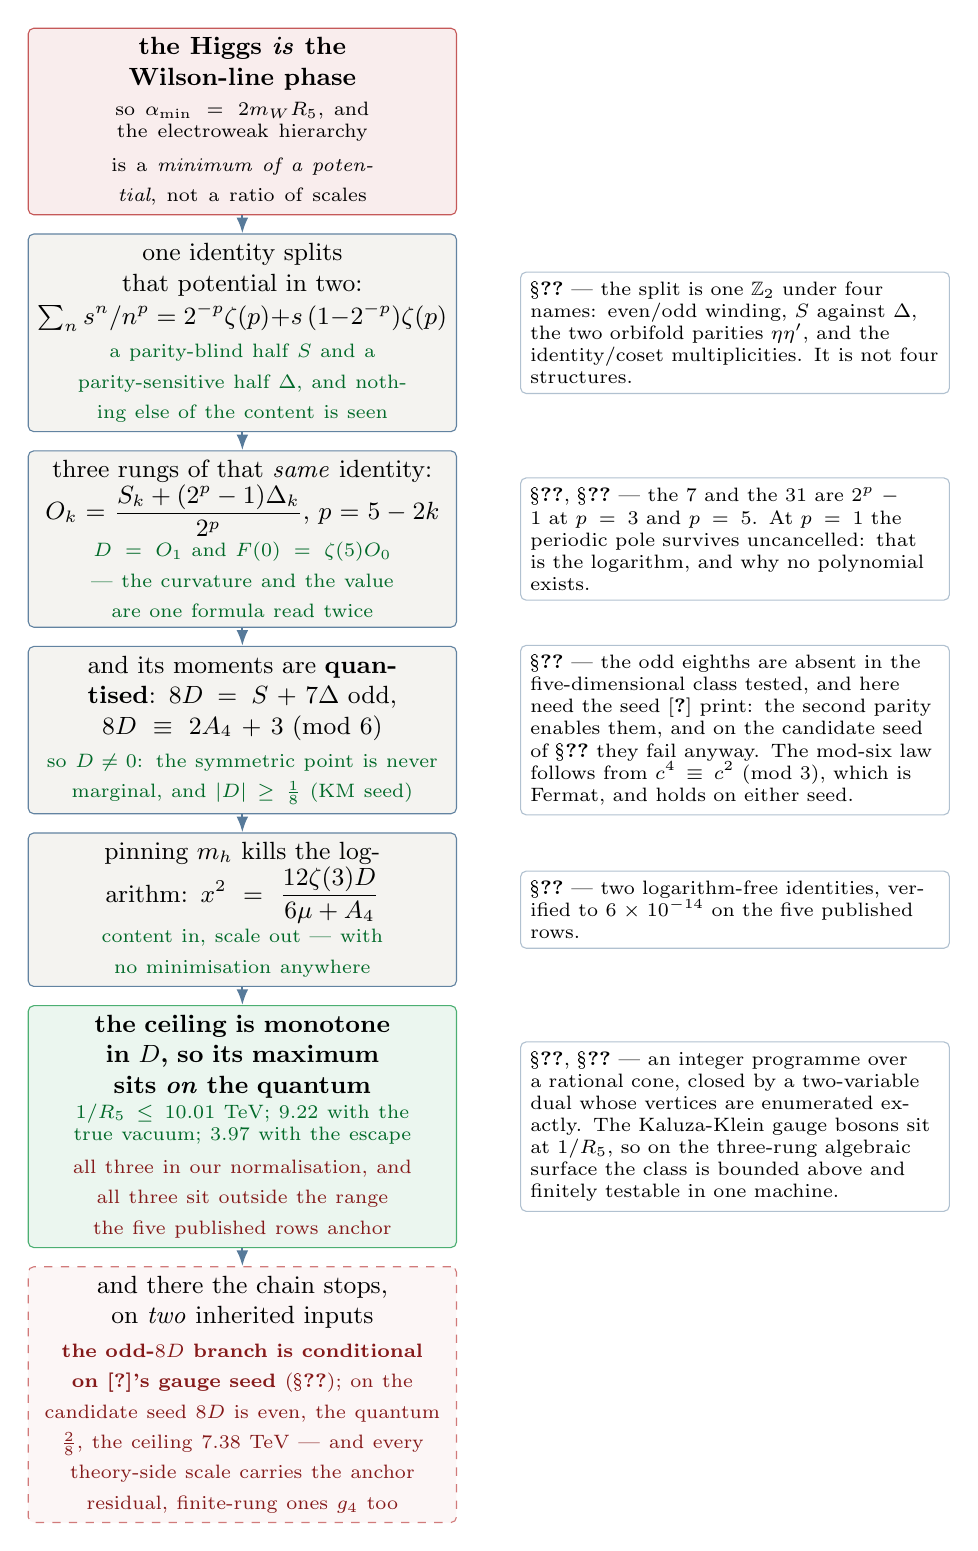
\begin{tikzpicture}[node distance=2.3mm, every node/.style={font=\small},
  bead/.style={draw=hdrblue!70,fill=softgrey,rounded corners=2pt,inner sep=3.4pt,
               minimum height=7mm,text width=52mm,align=center},
  root/.style={draw=warmred!75,fill=warmred!8,rounded corners=2pt,inner sep=3.4pt,
               minimum height=7mm,text width=52mm,align=center,font=\small\bfseries},
  gain/.style={draw=okgreen!70,fill=okgreen!8,rounded corners=2pt,inner sep=3.4pt,
               minimum height=7mm,text width=52mm,align=center},
  side/.style={draw=hdrblue!35,fill=white,rounded corners=2pt,inner sep=3.5pt,
               text width=52mm,align=left,font=\scriptsize},
  % the foot of the chain is not a link: it is where the chain ENDS, and it is dashed for
  % that reason.  Part VI carries the same box; a chain drawn without its own edge reads as
  % though it reached everything.
  edge/.style={draw=warmred!60,fill=warmred!4,rounded corners=2pt,inner sep=3.4pt,dashed,
               minimum height=7mm,text width=52mm,align=center},
  ar/.style={-{Latex[length=2mm]},hdrblue!75,thick}]

\node[root] (r) {the Higgs \emph{is} the Wilson-line phase\\[3pt]
  {\normalfont\scriptsize so $\amin=2m_WR_5$, and the electroweak hierarchy\\[1pt]
   is a \emph{minimum of a potential}, not a ratio of scales}};

\node[bead,below=of r] (id) {one identity splits that potential in two:\\[1pt]
  $\sum_n s^n/n^p=2^{-p}\zeta(p)+s\,(1-2^{-p})\zeta(p)$\\[1pt]
  \scriptsize\textcolor{okgreen!75!black}{a parity-blind half $S$ and a parity-sensitive half
  $\Delta$, and nothing else of the content is seen}};

\node[bead,below=of id] (lad) {three rungs of that \emph{same} identity:
  $O_k=\dfrac{S_k+(2^p-1)\Delta_k}{2^p}$, $p=5-2k$\\[1pt]
  \scriptsize\textcolor{okgreen!75!black}{$D=O_1$ and $F(0)=\zeta(5)O_0$ --- the curvature and the
  value are one formula read twice}};

\node[bead,below=of lad] (q) {and its moments are \textbf{quantised}:
  $8D=S+7\Delta$ odd, $8D\equiv2A_4+3\ (\mathrm{mod}\ 6)$\\[1pt]
  \scriptsize\textcolor{okgreen!75!black}{so $D\neq0$: the symmetric point is never marginal, and
  $|D|\ge\tfrac18$ \scriptsize(KM seed)}};

\node[bead,below=of q] (alg) {pinning $m_h$ kills the logarithm:
  $x^2=\dfrac{12\zeta(3)D}{6\mu+A_4}$\\[1pt]
  \scriptsize\textcolor{okgreen!75!black}{content in, scale out --- with no minimisation anywhere}};

\node[gain,below=of alg] (th) {\textbf{the ceiling is monotone in $D$, so its maximum sits
  \emph{on} the quantum}\\[1pt]
  \scriptsize\textcolor{okgreen!75!black}{$1/R_5\le10.01$~TeV; $9.22$ with the true vacuum;
  $3.97$ with the escape}\\[1pt]
  % los TRES, no los dos: la caja llevaba dos numeros cuando se escribio (524820c) y el 9.22
  % entro despues (e6766a3) sin que el conteo lo siguiera.  Un conteo en prosa es una afirmacion
  % y caduca cuando cambia la lista que cuenta.
  \scriptsize\textcolor{warmred!75!black}{all three in our normalisation, and all three sit outside
  the range the five published rows anchor}};

\node[edge,below=of th] (ed) {and there the chain stops, on \emph{two} inherited inputs\\[1pt]
  \scriptsize\textcolor{warmred!75!black}{\textbf{the odd-$8D$ branch is conditional on
  \cite{KM25}'s gauge seed} (\S\ref{sec:open}); on the candidate seed $8D$ is even, the quantum
  $\tfrac28$, the ceiling $7.38$~TeV --- and every theory-side scale carries the anchor
  residual, finite-rung ones $g_4$ too}};

\foreach \a/\b in {r/id,id/lad,lad/q,q/alg,alg/th} \draw[ar] (\a) -- (\b);
\draw[ar,dashed] (th) -- (ed);

\node[side,right=8mm of id]  (sid) {\S\ref{sec:ladder} --- the split is one $\ZZ_2$ under four
  names: even/odd winding, $S$ against $\Delta$, the two orbifold parities $\eta\eta'$, and the
  identity/coset multiplicities. It is not four structures.};
\node[side,right=8mm of lad] (sla) {\S\ref{sec:ladder}, \S\ref{sec:arith} --- the $7$ and the $31$
  are $2^p-1$ at $p=3$ and $p=5$. At $p=1$ the periodic pole survives
  uncancelled: that is the logarithm, and why no polynomial exists.};
\node[side,right=8mm of q]   (sq)  {\S\ref{sec:arith} --- the odd eighths are absent in the
  five-dimensional class tested, and here need the seed \cite{KM25} print: the second parity
  enables them, and on the candidate seed of \S\ref{sec:open} they fail anyway. The mod-six law follows from $c^4\equiv c^2\ (\mathrm{mod}\
  3)$, which is Fermat, and holds on either seed.};
\node[side,right=8mm of alg] (sal) {\S\ref{sec:ceiling} --- two logarithm-free identities, verified
  to $6\times10^{-14}$ on the five published rows.};
\node[side,right=8mm of th]  (sth) {\S\ref{sec:ceiling}, \S\ref{sec:pred} --- an integer programme
  over a rational cone, closed by a two-variable dual whose vertices are enumerated exactly. The
  Kaluza-Klein gauge bosons sit at $1/R_5$, so on the three-rung algebraic surface the class is
  bounded above and finitely testable in one machine.};
\end{tikzpicture}
\caption{\textbf{The chain, and it is one chain.} Every link is an identity rather than a step. The
Higgs being a phase makes the hierarchy a vacuum; one Bernoulli-free identity splits that vacuum's
potential into a parity-blind and a parity-sensitive moment and sees nothing else of the content;
the value, the curvature and the fourth moment are that one identity at $p=5,3,1$; the resulting
invariant is quantised, and \emph{oddly} so on the seed \cite{KM25} print, which is what keeps it
from zero; pinning the measured Higgs mass then removes the
logarithm and leaves the scale as an algebraic function of two moments; and because the ceiling is
monotone in $D$, the quantisation is what puts its maximum on the smallest allowed $D$ ---
Theorem~\ref{thm:eighths} doing physical work rather than arithmetic. The red note is the scope that
travels with both numbers; the dashed box at the foot is not a link but the edge of the
chain.}\label{fig:chain}
\end{figure}

\bridge{Before any of it: which equations are inherited, which are ours, and the one caveat that
every theory-side scale in this paper carries.}

% ===================================================================
\section{What is inherited, and what is computed}\label{sec:setting}

The model of \cite{KM25} is six-dimensional $\su7$ on $S^1/\ZZ_2\times S^1/\ZZ_2$. Its
five-dimensional ancestor is \cite{KTY17}; its six-dimensional sibling is the $\su4$
construction of \cite{AHMN} on $T^2/\ZZ_2$, which predicts $\sin^2\theta_W = 1/4$ at the
compactification scale and is the control \S\ref{sec:open} uses for the degree-of-freedom
count. \cite{KM25}'s orbifold parities are their
eqs.~(11)--(13). Their one-loop potential, their eqs.~(63)--(68), is a sum over the bulk content of
polylogarithms of the Wilson-line phase; in the form we use it,
\begin{equation}\label{eq:F}
  F(\alpha)\;=\;\sum_{\text{terms}} m\,\mathrm{Re}\,\mathrm{Li}_5\!\left(s\,e^{\,i c \pi \alpha}\right),
  \qquad c\in\ZZ,\quad s=\pm1,
\end{equation}
\noindent \textbf{And \eqref{eq:F} is already an approximation, inherited rather than made here,
which has to be said before anything is called exact.} \cite{KM25}'s potential before their
eqs.~(68) and (71) carries $\coth(\pi k n)$ and $\mathrm{csch}(\pi k n)$ with
$k=R_5/R_6$, and the $n^{-5}$ form is what those become as $k\to\infty$; their model takes
$R_5\gg R_6$ throughout, with $1/R_6$ a free parameter they suggest may be the Planck scale.
\textbf{So everywhere below, ``exact'' means exact with respect to \eqref{eq:F}}, the potential of
\cite{KM25} already reduced in that limit, and never with respect to the full six-dimensional one.
The correction is suppressed by $e^{-2\pi k}$ and is numerically nothing for any $1/R_6$ the model
wants; what it changes is the \emph{status} of several statements, and they are stated with that
scope. In particular Theorem~\ref{thm:complete}'s five coordinates are complete for the $\mathrm{Li}_5$
space of \eqref{eq:F}, not for the full winding weight, which mixes powers and does not close on
five --- \S\ref{sec:ceiling} says so where the function space is counted, and it is the same caveat.

\noindent \textbf{And ``bulk content'' means one thing throughout, so it is worth fixing here.} It
is a vector of non-negative multiplicities over the \emph{eight} $(\text{representation},
\text{parity})$ pairs of \cite{KM25}'s Table~1 --- $\rep7$, $\rep{28}$, $\rep{48}$, $\rep{84}$ at
two parities each. Arbitrary below always means arbitrary in the multiplicities, never in the list.
That distinction earns a sentence because \S\ref{sec:ceiling} removes a cap on the \emph{size} of
the content and this one, on its \emph{type}, stays: the Wilson line sees a weight through
$c=2|q|$ with $q$ set by the number of index-$7$ boxes, so $c\le3$ here \emph{because their largest
representation has three boxes} --- checked against the term tables themselves in
\texttt{content\_\allowbreak scope.py} --- and nothing in the model, the orbifold or the potential
caps the box count. A bulk field in a four-box representation of $\su7$ would bring $c=4$, and it
would move two things: $A_4$ collects $mc^4$, so a charge-four state is worth $256$ against a
charge-three state's $81$ and the certificate of \S\ref{sec:ceiling} would run over a different
cone; and the function space of \S\ref{sec:closed} would grow, because the duplication chain that
stops at $c=3$ would continue, taking eight functions to six dimensions instead of six to five.
Theorem~\ref{thm:complete} is therefore a statement about \emph{this} charge alphabet. None of that
is a defect of what follows; all of it is scope, and scope has to be printed.

\noindent Each bulk multiplet contributes a table of terms $(m,s,c)$: an integer charge $c$ under the
Wilson-line direction, a sign $s$ recording whether that state's Kaluza-Klein tower is periodic or
antiperiodic, and a multiplicity $m$. The gauge sector contributes
$(-1,+1,2)$, $(-2,+1,1)$, $(-\tfrac72,-1,1)$, and those three multiplicities are \emph{reconstructed} from
their eqs.~(63)--(67) rather than assumed --- inferred backwards from their coefficients, never
derived forwards from the geometry (\S\ref{sec:open}): Part~VI reconstructs the three coefficients of their
eq.~(68) from two unknowns. Three equations for two unknowns is overdetermined, so it could have
failed --- but only in one place. Two of the three rows contain no $P_6=-1$ pair at all, so the
spare equation tests the \emph{periodic} weight and nothing else. The antiperiodic weight is fixed
once and checked never. Both weights carry below, and it takes both: what decides the parity is
$2n_++\tfrac12 n_-$ over the row that mixes them, which needs the periodic part even \emph{and} the
antiperiodic part odd.

\paragraph{The moments.} Writing $A_2=\sum_{s=+1} m c^2$, $B_2=\sum_{s=-1} m c^2$,
$A_4=\sum_{s=+1} m c^4$, $B_4=\sum_{s=-1} m c^4$ and $A_4^{L}=\sum_{s=+1} m c^4\ln c$, the three
combinations that this paper is about are
\begin{equation}\label{eq:moments}
  D \;=\; A_2-\tfrac34 B_2\,,\qquad
  A_4\,,\qquad
  G \;=\; A_4 H_4 - A_4^{L} - \ln 2\,B_4\,,\qquad H_4=\tfrac{25}{12}\,.
\end{equation}
$D$ is Part~VI's curvature at the symmetric point, $V''(0)=-\pi^2\zeta(3)D$; the factor $\tfrac34$
is $\eta(3)/\zeta(3)$ and comes from their eq.~(67), not from a choice of ours.

\paragraph{The caveat, stated once and carried to the end.} Part~VI \S7 records an unresolved
discrepancy: our assembly of their potential does not reproduce their published $\amin$ column. The
row-wise ratio $\amin^{\text{ours}}/\amin^{\text{theirs}}$ runs from $1.03$ to $2.08$; grouped, it is
$1.94$ on the two rows containing a $\rep{48}$ and $1.20$ on the other three. That question is not
settled here, and \S\ref{sec:anchor} does not settle it either --- but it does move it: the second
anchor validates the potential and the minimiser in the \emph{periodic} $B=0$ sector against a
different published computation, which narrows what remains to be explained to the model-specific
dictionary \emph{or} to the antiperiodic sector, which no published check anchors and
\S\ref{sec:open} says why.
\textbf{Every scale below that is inferred through the Higgs-potential dictionary carries that
residual}, which is every absolute number on the theory side of this paper. It is \emph{not}
the collider recast of \S\ref{sec:collider}: \eqref{eq:tulimit}'s $10.86$~TeV and the $13.75$
beside it are read off \cite{CMSangular}'s data through the tower's form factor and never pass
through $\amin$ at all. The comb they are read \emph{at}, \eqref{eq:combchi}, is theory-side
and does carry it. What also does not carry it is the
\emph{matter} sublattice of \S\ref{sec:arith}: the eight generators are group theory, and the
anchor residual cannot touch them. The affine offset those generators are added to is a separate
matter, and it is \S\ref{sec:open}'s --- \emph{the lattice is a property of the content; the coset
it sits in is a property of the gauge seed}, and the distinction is not pedantic, because moving
only the base point is exactly what turns $8D$ from odd to even.

\paragraph{And the residual is not a \emph{band}, which changes how far it may be carried.} A band is unexplained
scatter and propagates as a multiplier. This does not scatter: sorted by $D$ the five ratios fall
$2.076,\,1.803,\,1.286,\,1.286,\,1.025$, monotonically and with the tie in $D$ carrying a tie in the
ratio --- an ordering shared by only $2$ of the $120$ pairings of these five ratios to these five
rows, so $p=0.017$. It is a trend in the content, and it rises as $D$ falls. Two consequences, and
both bear on \S\ref{sec:ceiling}. First, \emph{which} moment drives it is not decided here: $A_4$
orders the same five rows exactly as well as $D$ does, the two being nearly collinear over them, and
five points cannot separate them. Second, and this is the sharp one, the ratio may only be carried
to contents the five rows actually surround. They anchor $D\in[1.125,3.625]$ and
$A_4\in[189,271]$; the ceiling of \S\ref{sec:ceiling} is certified at $(A_4,8D)=(215,1)$, whose $D$
is nine times below the smallest anchored one, and the escape ceiling at $(727,11)$, whose $A_4$ is
$2.7$ times the largest. \textbf{Each ceiling is anchored in one moment and unanchored in the
other}, and with the two moments unseparated neither can inherit the range as an uncertainty.
Where a rescaled number appears below it is therefore labelled an extrapolation, not a bound.
Measured in \texttt{anchor\_trend.py}.

\bridge{And now the structural question, which decides what kind of answer is available at all: why
is there no exact formula for this vacuum, when the analogous thermal problem has had one since 1981?}

% ===================================================================
\section{Why there is no polynomial: Bernoulli against Clausen}\label{sec:parity}

A Wilson-line potential is a \emph{holonomy} potential. It is the same object Gross, Pisarski and
Yaffe wrote for a gauge theory at finite temperature \cite{GPY}: a sum over windings of the compact
direction, weighted by the holonomy eigenvalues. The two problems differ in one index, and the index
decides whether the answer is a polynomial.

The classical fact is a Fourier series. For $0\le x\le 1$,
\begin{equation}\label{eq:bernoulli}
  \sum_{n\ge1}\frac{\cos 2\pi n x}{n^{2k}}
   \;=\;\frac{(-1)^{k+1}(2\pi)^{2k}}{2\,(2k)!}\,B_{2k}(x)\,,
\end{equation}
a polynomial with rational coefficients; while the same series with an \emph{odd} exponent is a
Clausen function, for which no such expression is known. The tell is the value at $x=0$: for even
$p$, $\zeta(p)/\pi^p\in\mathbb{Q}$ is a theorem; for odd $p$ it is not known either way, and an
integer-relation search at $40$ digits finds no relation for $\zeta(3)$ or $\zeta(5)$ while
returning $1/6$, $1/90$ and $1/945$ for $\zeta(2)$, $\zeta(4)$ and $\zeta(6)$. \textbf{That
asymmetry is evidence and motivation, not proof}, and it is not what the section rests on: a
$40$-digit null is a statement about a search, and while $\zeta(3)$ itself is irrational
\cite{Apery}, the irrationality of $\zeta(3)/\pi^3$ does not follow and is open.
What is rigorous is one line further down --- the $p=5$ potential carries an $x^4\ln x$ branch
point, established in \S\ref{sec:ladder} from the expansion itself, and \emph{no polynomial has a
branch point}. The arithmetic of $\zeta(3)$ and $\zeta(5)$ says why one should have expected it;
the branch point is why there cannot be one.

A gauge theory in $d$ dimensions with one compact direction contributes
$\sum_n \cos(2\pi n x)/n^{d}$. Hence:

\begin{center}\small
\rowcolors{2}{white}{softgrey}
\begin{tabular}{lccl}
\toprule
\rowcolor{hdrblue!10}theory & index & parity & closed form of the holonomy potential\\
\midrule
\rowcolor{okgreen!12}four-dimensional, finite temperature & $4$ & even & $B_4(x)=x^2(1-x)^2-\tfrac1{30}$ --- \textbf{exact}\\
\rowcolor{amber!12}five-dimensional on $S^1$ \cite{vGIQ,HY04} & $5$ & odd & Clausen; $\zeta(5)$, $\zeta(3)$; no polynomial\\
\rowcolor{amber!12}six-dimensional on $S^1\times S^1$ \cite{KM25} & $5$ & odd & the same\\
\bottomrule
\end{tabular}
\end{center}

\noindent and the Gross-Pisarski-Yaffe quartic is recovered from \eqref{eq:bernoulli} to $10^{-41}$
by the ancillary script.

\begin{keyeq}
\textbf{The ladder of this paper is $p=5-2k$, so it runs $5,\,3,\,1$: odd, odd, odd.} Stepping by
two from an odd start cannot reach the solvable case. There is no rung at which this potential
becomes a polynomial, and the last rung is the pole of $\zeta$ --- which is exactly where the
$\alpha^4\log\alpha$ branch point of \S\ref{sec:closed} comes from.
\end{keyeq}

This is worth stating plainly because it explains a literature gap rather than merely noting one.
The finite-temperature community never needed an expansion of the holonomy potential: it has the
polynomial, and every question about the vacuum is algebra. The extra-dimensional community works at
an odd index, has no polynomial, and computes numerically model by model. A closed form for the
vacuum is the object that is missing, and the reason it is missing is arithmetic rather than technical.
Figure~\ref{fig:parity} carries both halves of that: the quartic that exists at $p=4$, and the
integer-relation search that finds nothing at $p=5$.

\begin{figure}[t]\centering
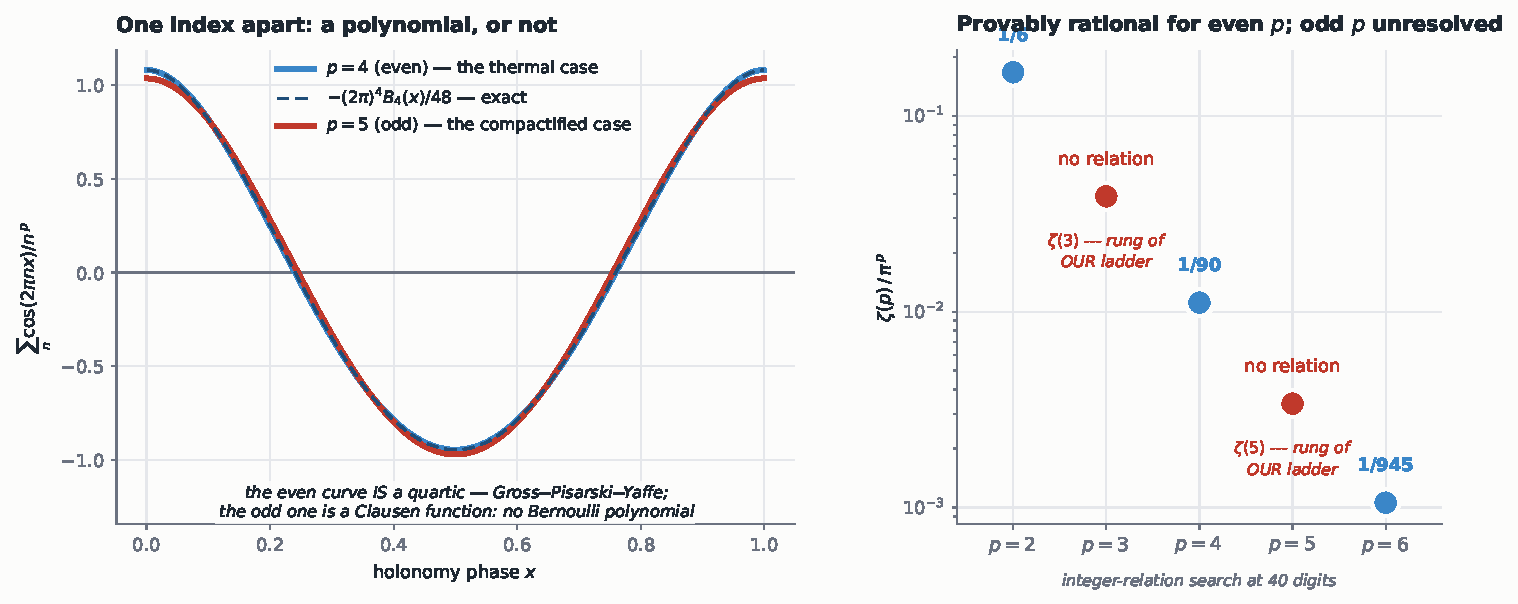
\includegraphics[width=\textwidth]{fig_parity.pdf}
\caption{\textbf{One index apart.} The same Fourier sum at an even and an odd exponent. At $p=4$ it \emph{is} a quartic --- the dashed curve is $-(2\pi)^4B_4(x)/48$, the Gross-Pisarski-Yaffe potential, and the two coincide to $10^{-41}$. At $p=5$ no such expression exists. Right: the arithmetic tell. $\zeta(p)/\pi^p$ is rational for even $p$, a theorem; for odd $p$ it is open, and an integer-relation search at $40$ digits returns $1/6$, $1/90$ and $1/945$ and finds nothing for $\zeta(3)$ or $\zeta(5)$ --- which are the two rungs of our ladder. Evidence, not proof: what rules out a polynomial rigorously is the $x^4\ln x$ branch point.}\label{fig:parity}
\end{figure}

\bridge{With the shape of the answer settled, the expansion itself: one series, read rung by rung,
each pairing a moment of the content against a zeta value. Three rungs carry the physics, and where
the fourth would go there is a pole --- which turns out to be the last place a new transcendental
can enter.}

% ===================================================================
\section{One expansion, three rungs}\label{sec:ladder}

Expanding \eqref{eq:F} in the phase is a single operation:
\begin{equation}\label{eq:expansion}
  \mathrm{Re}\,\mathrm{Li}_5\!\left(s\,e^{ic\pi\alpha}\right)
  \;=\;\sum_{k\ge0}\frac{(-1)^k (c\pi\alpha)^{2k}}{(2k)!}\;\sum_{n\ge1}\frac{s^n}{n^{5-2k}}\,,
\end{equation}
so the $2k$-th derivative in $\alpha$ is governed by $p=5-2k$ \emph{and} by the $2k$-th moment of the
content. The inner sum splits once and for all, because $s^n=+1$ on even windings whatever $s$ is:
\begin{equation}\label{eq:split}
  \sum_{n\ge1}\frac{s^n}{n^{p}}\;=\;2^{-p}\zeta(p)\;+\;s\,(1-2^{-p})\,\zeta(p)\,.
\end{equation}
Summed over the content, the two brackets collect the two moments at once --- one blind to the
parity, one weighted by it --- and the rung-$k$ coefficient is, with the last column of the table
below read on the gauge seed \cite{KM25} print,
\begin{equation}\label{eq:rung}
  \frac{S_k+(2^{p}-1)\,\Delta_k}{2^{p}}\,,\qquad
  S_k=\sum m\,c^{2k}\,,\qquad \Delta_k=\sum m\,c^{2k}s\,.
\end{equation}

\begin{center}\small
\rowcolors{2}{white}{softgrey}
\begin{tabular}{ccll r}
\toprule
\rowcolor{hdrblue!10}$k$ & $p$ & object & coefficient & gauge sector\\
\midrule
$0$ & $5$ & the \emph{value} $F(0)$ & $(S_0+31\Delta_0)/32$ & $9$\\
\rowcolor{amber!14}$1$ & $3$ & the \emph{curvature} $V''(0)=-\pi^2\zeta(3)D$ & $(S_1+7\Delta_1)/8$ & $-27$\\
$2$ & $1$ & the fourth moment & $(S_2+\Delta_2)/2=\mathcal{A}_2=A_4$ --- periodic only & $-36$\\
\bottomrule
\end{tabular}
\end{center}

\noindent The eighths of Part~VI are $2^3$ and its seven is $2^3-1$; the denominators $32,8,2$ are
$2^p$. At $p=1$ both halves of \eqref{eq:split} diverge, and what becomes of them depends on the
parity: at $s=-1$ they cancel and leave a \emph{finite} $-\ln2$, while at $s=+1$ they add and the
pole survives. \textbf{So the $x^4\ln x$ is the \emph{periodic} sector's uncancelled pole}, and the
antiperiodic sector contributes instead the $\ln2$ that \eqref{eq:moments} carries on $B_4$.
$\mathrm{Li}_5$ has exactly one logarithm in $x$, and it is periodic-only --- which is the $p=1$
row of the table above, read as an analytic statement rather than a bookkeeping one.

\paragraph{The ladder is geometric, and charge two is its fixed point.} Since $2^{p}=32/4^{k}$, a
single term $(m,s,c)$ walks the ladder as a geometric sequence:
\begin{keyeq}
\begin{equation}\label{eq:modes}
  s=+1:\;\; 32\,m\,\sigma^k \;\;\text{with}\;\;\sigma=\tfrac{c^2}{4};
  \qquad
  s=-1:\;\; 2\,m\,(c^2)^k - 32\,m\,\sigma^k \;\;\text{--- two modes.}
\end{equation}
\end{keyeq}
So $O_k=\sum_\sigma A_\sigma\,\sigma^k$, with $\sigma\in\{\tfrac14,1,\tfrac94\}$ from $c=1,2,3$ and,
for antiperiodic states only, additionally $\sigma\in\{1,4,9\}$.

\begin{keyeq}
A \emph{charge-two} periodic state has $\sigma=1$: it weighs exactly the same on the value, on the
curvature and on the fourth moment. Charge one decays by four per rung; charge three grows. The
gauge sector reaches only $\{\tfrac14,1\}$, so its ladder has two parameters rather than three, and
\[
  O(5)-O(3)\;=\;4\,\bigl[\,O(3)-O(1)\,\bigr]
\]
identically --- zero counterexamples over all $4096$ admissible parity assignments. Its two
amplitudes are computed in \S\ref{sec:arith}, \eqref{eq:gaugerung}, where the identity becomes a
line of algebra rather than a census.
\end{keyeq}

The geometric relation survives any matter content that opens no third mode, and dies as soon as one appears.
Predicted before the table was computed and confirmed on all eight multiplets: it holds for
$\rep7^{(\pm)}$, $\rep{28}^{(+,+)}$ and $\rep{48}^{(+,+)}$, and breaks for $\rep{28}^{(+,-)}$ and
$\rep{48}^{(+,-)}$ --- which differ from their partners only by whether their charge-two state is
periodic or antiperiodic --- and for both $\rep{84}$s, the only multiplets carrying a charge three.
Every row of their Table~1 contains an $\rep{84}$, so for every published row the value, the
curvature and the fourth moment are three independent numbers; without one, they are two.

\paragraph{And that last difference is sharper than it looks: the charge-two parity flip is
the only log-free one.} Move one unit of
multiplicity at charge $c$ from the periodic tower to the antiperiodic one. The three moments shift
by
\[
  \Delta D=-\tfrac74c^2,\qquad \Delta A_4=-c^4,\qquad
  \Delta G=-c^4\Bigl(H_4-\ln\tfrac{c}{2}\Bigr),
\]
and $\Delta G$ is \emph{rational} exactly when $c=2$, because $\ln c$ is then the same $\ln2$ that
the antiperiodic tower carries universally in \eqref{eq:moments}. So at charge two, and at no other
charge, the parity flip is log-free, with the exact signature
\begin{equation}\label{eq:c2flip}
  (\Delta D,\;\Delta A_4,\;\Delta G)\;=\;\bigl(-7,\;-16,\;-\tfrac{100}{3}\bigr)\ \text{per unit,}
\end{equation}
and, equivalently, $J\equiv G-H_4A_4=-A_4^{L}-\ln2\,B_4$ is completely blind to the parity of a
charge-two state. That this is the same charge that sits at the fixed point of \eqref{eq:modes} is
not a consequence of it: $\sigma=1$ is about $c^2/4$ and this is about $\ln(c/2)$, and the two
coincide only because both ask $c$ to be $2$.

It suggested a test of Part~VI's anchor residual, since the rows that fail are the ones containing a
$\rep{48}$ and the parity of a charge-two state is what distinguishes $\rep{28}^{(+,+)}$ from
$\rep{28}^{(+,-)}$ and $\rep{48}^{(+,+)}$ from $\rep{48}^{(+,-)}$: if the residual were a misread
charge-two parity, then their published $(\amin,m_h)$ would sit at our moments shifted by an
integer multiple of \eqref{eq:c2flip}. Solving that multiple from (II) and then checking (I), which
the solve never saw, gives non-integer multiples between $0.03$ and $0.15$ and residuals in (I) of
order $10^{-1}$ to $1$; two decoy vectors, the log-carrying $c=1$ and $c=3$ flips, do no worse.
\textbf{The test is negative and the reading is withdrawn}: whatever the anchor residual is, it is
not a charge-two parity. It is recorded because the vector is exact and cheap to re-test against any
future candidate.

But the log-free property itself outlives the test it was invented for, and it is not an accident
of $c=2$ being small. \S\ref{sec:ceiling} writes $G$ in the basis $\{1,\ln2,\ln3\}$ and finds the
content sitting on a \emph{four}-dimensional lattice whose logarithmic coordinates are the $\ln2$
and $\ln3$ weights $U$ and $V$. In that lattice the charge-two flip is the move with $\Delta U=\Delta V=0$ --- the
unique generator direction the third axis cannot see --- and \emph{that} is why its $\Delta G$ came
out rational: with no logarithm moving, $\Delta G$ can only be $\tfrac{25}{12}\Delta A_4$, which is
$-\tfrac{100}{3}$. Measured in \texttt{crossed\_\allowbreak equations.py} and
\texttt{semigroup.py}.

\paragraph{The top rung is not ours, and neither is more of it than we first took.} Cacciapaglia
\emph{et al.}~\cite{CCD24} decide orbifold stability by comparing the potential at $a=0$ and
$a=1/2$, and their eqs.~(2.11)--(2.13) give $F_-(0)=-\tfrac{15}{16}F_+(0)$, with
$\tfrac{15}{16}=\eta(5)/\zeta(5)$, the sign deciding whether the orbifold is stable --- a weight
already in print in \cite{PP01} eq.~(13) in 2001, as
$V^{-,\text{scalar}}=-\tfrac{15}{16}V^{+,\text{scalar}}$. The \emph{split} it comes from is in six
dimensions too, in \cite{GHBQ05} eq.~(3.18), where the two orbifold parities enter as
$\mathrm{Li}_n(\pm q)$ --- but not the weight: that paper never evaluates the ratio, and the
strings $15/16$, $31/32$ and $\zeta(5)$ do not occur anywhere in its forty pages.
\textbf{The parity-split architecture is theirs and is not claimed here.} And their eq.~(2.11) says
more than that value: $F_-(a)=-F_+(a)+\tfrac1{16}F_+(2a)$ is an identity in $a$, the duplication
formula \cite{Wood} rather than \eqref{eq:split} at a point, and \S\ref{sec:closed} uses it as such.
Read only at $a=0$ it is the top rung; read as a function it is why the potential spans five. What their method does not reach is the curvature: over $45$ pages
the words \emph{curvature} and \emph{second derivative} do not occur, nor \emph{Dynkin} nor
\emph{trace}, and their single second derivative (their eq.~(3.15)) is taken in an example where the
potential has already collapsed to one term, so no parity split appears in it. Their own text says
why they do not go there: small vacuum expectation values, they write, are ``usually obtained via
some form of fine tuning'' --- and the small-$\alpha$ interior minimum they set aside is precisely
the regime of \cite{KM25} and of this paper. \S\ref{sec:novel} states the boundary in full.

\textbf{Their stability criterion is theirs too}, and it returns in \S\ref{sec:ceiling}: comparing
the potential at the two symmetric points is what decides whether the small-$\alpha$ minimum this
paper computes is the vacuum or merely a vacuum, and \cite{CCD24} state it, prove the identities it
needs and draw its sign rule. \eqref{eq:truevac} is that statement summed over a bulk content, in
our notation and with nothing added. The one thing that is ours is the use: summed, it is
\emph{linear} in the multiplicities, so it can go inside the integer program that produces the
ceiling --- and the ceiling is computed twice for exactly that reason, the two answers differing by
$0.8$~TeV.
Figure~\ref{fig:ladder} is the rung structure the curvature adds, with the gauge sector's own three
rungs beside it.

\begin{figure}[t]\centering
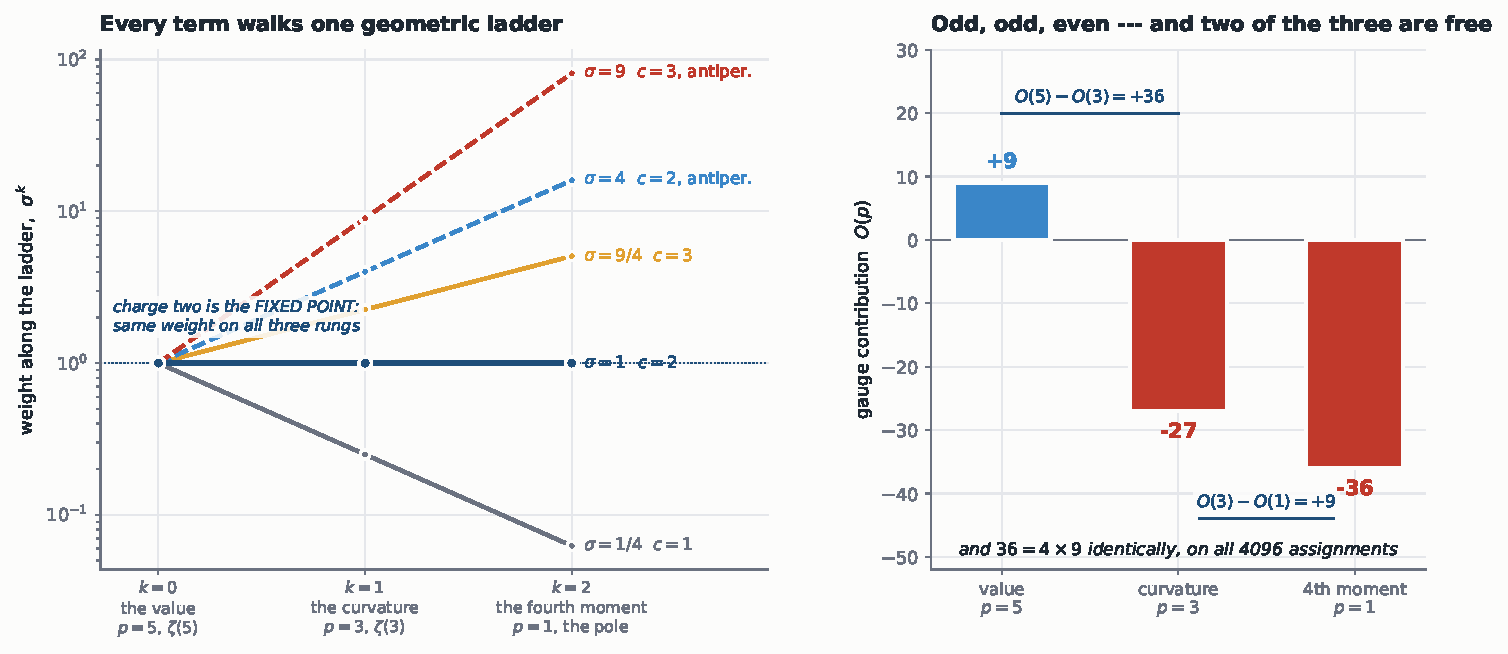
\includegraphics[width=\textwidth]{fig_ladder.pdf}
\caption{\textbf{The ladder is geometric.} Left: every term of the potential walks the three rungs as $\sigma^k$ with $\sigma=c^2/4$, and antiperiodic terms carry a second mode $\sigma=c^2$. A periodic charge-two state has $\sigma=1$: it weighs the same on the value, the curvature and the fourth moment, and is the flat spine everything else fans away from. Right: the gauge sector's own three rungs on the seed \cite{KM25} print, odd, odd and even. It reaches only $\sigma\in\{1/4,1\}$, so two of the three numbers determine the third --- on every one of the $4096$ admissible parity assignments.}\label{fig:ladder}
\end{figure}

\bridge{The curvature rung is where the vacuum is decided, so that is the rung to solve.}

% ===================================================================
\section{The hierarchy in closed form}\label{sec:closed}

Keeping the three rungs of \S\ref{sec:ladder} and writing $x=\pi\alpha$,
\begin{equation}\label{eq:Fexp}
  F(x)\;=\;\text{const}\;-\;\frac{\zeta(3)D}{2}\,x^2\;+\;\frac{x^4}{24}\bigl[\,G-A_4\ln x\,\bigr]
  \;+\;O(x^6)\,,
\end{equation}
the logarithm being the $p=1$ rung. The symmetric point is therefore \emph{stationary but not
analytic}: $x^4\ln x$ and its first two derivatives vanish at the origin, so $F'(0)=0$ and
$F''(0)=-\zeta(3)D$ are perfectly well defined --- which is what entitles
Theorem~\ref{thm:eighths} to speak of the curvature there at all --- while the branch point sits
two derivatives higher up and no ordinary Taylor series exists. And $\mathrm{d}F/\mathrm{d}x=0$
gives, not a root of a polynomial, but
\begin{keyeq}
\begin{equation}\label{eq:amin}
  x^2 \;=\; \frac{24\,\zeta(3)\,D}{\,4G - A_4\,(4\ln x + 1)\,}\,,\qquad x=\pi\amin .
\end{equation}
\end{keyeq}

\noindent The hierarchy is a ratio of two moments of the content, corrected by a third.

\paragraph{And it is a closed form, which we had been calling a fixed point.} Earlier versions of
this paper solved \eqref{eq:amin} by iteration and described it as a fixed-point equation rather
than a solvable one. It is solvable. Putting $y=x^2$, so that $\ln x=\tfrac12\ln y$, it is
$y\,(b-\ln y)=d$ with $b=(4G-A_4)/(2A_4)$ and $d=12\zeta(3)D/A_4$; setting $u=\ln y-b$ turns that
into $u\,e^{u}=-d\,e^{-b}$, which is the definition of the Lambert $W$ function. Hence
\begin{keyeq}
\begin{equation}\label{eq:lambert}
  x^{2}\;=\;\frac{-d}{W\!\left(-d\,e^{-b}\right)}\,,\qquad
  b=\frac{4G-A_4}{2A_4}\,,\qquad d=\frac{12\,\zeta(3)\,D}{A_4}\,.
\end{equation}
\end{keyeq}
A negative argument is necessary for two real branches and not sufficient: $W$ is real only for
$z\ge-1/e$, which here reads $b-1-\ln d\ge0$. That condition holds on every content used here,
and it is not an extra hypothesis. \textbf{Which branch is the minimum is not a labelling but a
theorem}, and one line of algebra: eliminating $x^2$ between \eqref{eq:lambert} and identity~(II)
of \eqref{eq:two} gives
\begin{equation}\label{eq:branchmu}
  \mu\;=\;-\frac{A_4}{6}\,(W+1)\,,\qquad\text{equivalently}\qquad W_{-1}=-1-\frac{6\mu}{A_4}\,,
\end{equation}
with $\mu=m_h^2/(K\pi^2)^2$. Since $A_4>0$, the branch with $W\le-1$ carries $\mu\ge0$ and the
branch with $-1<W<0$ carries $\mu<0$: \emph{the sign of the Higgs mass squared is the sign of
$-(W+1)$}. So $W_{-1}$ is the minimum and $W_{0}$ a maximum, proved rather than assigned; on the
five published rows $\mu$ runs $81$ to $115$ on the first and $-30$ to $-38$ on the second. It
also says the measured Higgs mass \emph{selects a point of the Lambert sheet}, and that $m_h\to0$
is $W\to-1$ --- the branch point, which is the fold Theorem~\ref{thm:eighths} is careful not to
claim. Verified in \texttt{lambert\_\allowbreak criticality.py}. \textbf{Neither is one of the two symmetric
points $\alpha=0,1$ that \S\ref{sec:ceiling} compares}: those are endpoints of the domain, their
difference \eqref{eq:truevac} is evaluated exactly and not through this expansion, and the outer
root plays no part in the ceiling. Checked against the iteration on the five
published rows, agreeing to $1.8\times10^{-14}$, in \texttt{lambert\_\allowbreak amin.py}. We owe
a piece of our own narrative with it: \S\ref{sec:parity} rules
out a \emph{polynomial}, which the branch point does rigorously, and that is all it rules out. It
never ruled out a closed form, and the same $W$ was already in this paper one section
later, at \eqref{eq:rinf}, before the equation it belongs to was recognised.

\paragraph{And in the right coordinates the whole family is one picture.} Put
$L=b-1-\ln d$, the discriminant itself --- two real branches exist exactly when $L\ge0$. Then
$b=L+1+\ln d$ and the argument of the Lambert function loses its second parameter outright,
$z=-d\,e^{-b}=-e^{-(1+L)}$, so \eqref{eq:lambert} separates:
\begin{equation}\label{eq:foldsep}
  x^{2}\;=\;d\;f(L),\qquad f(L)=\frac{-1}{W\!\left(-e^{-(1+L)}\right)}\,,
\end{equation}
one factor per coordinate. The two branches are then two sheets of one surface over $(L,d)$, and
they meet where $W=-1$, that is $f=1$, that is the \emph{straight} edge $L=0$ --- along the whole of
which $\mu=0$ by \eqref{eq:branchmu}. \textbf{The closed form is the upper sheet of a fold, and the
Higgs mass is the height above its edge.} Figure~\ref{fig:lambert} is that surface, with their five
published rows and the vertex where \S\ref{sec:ceiling}'s ceiling is attained standing on it.

\begin{figure}[t]
\centering
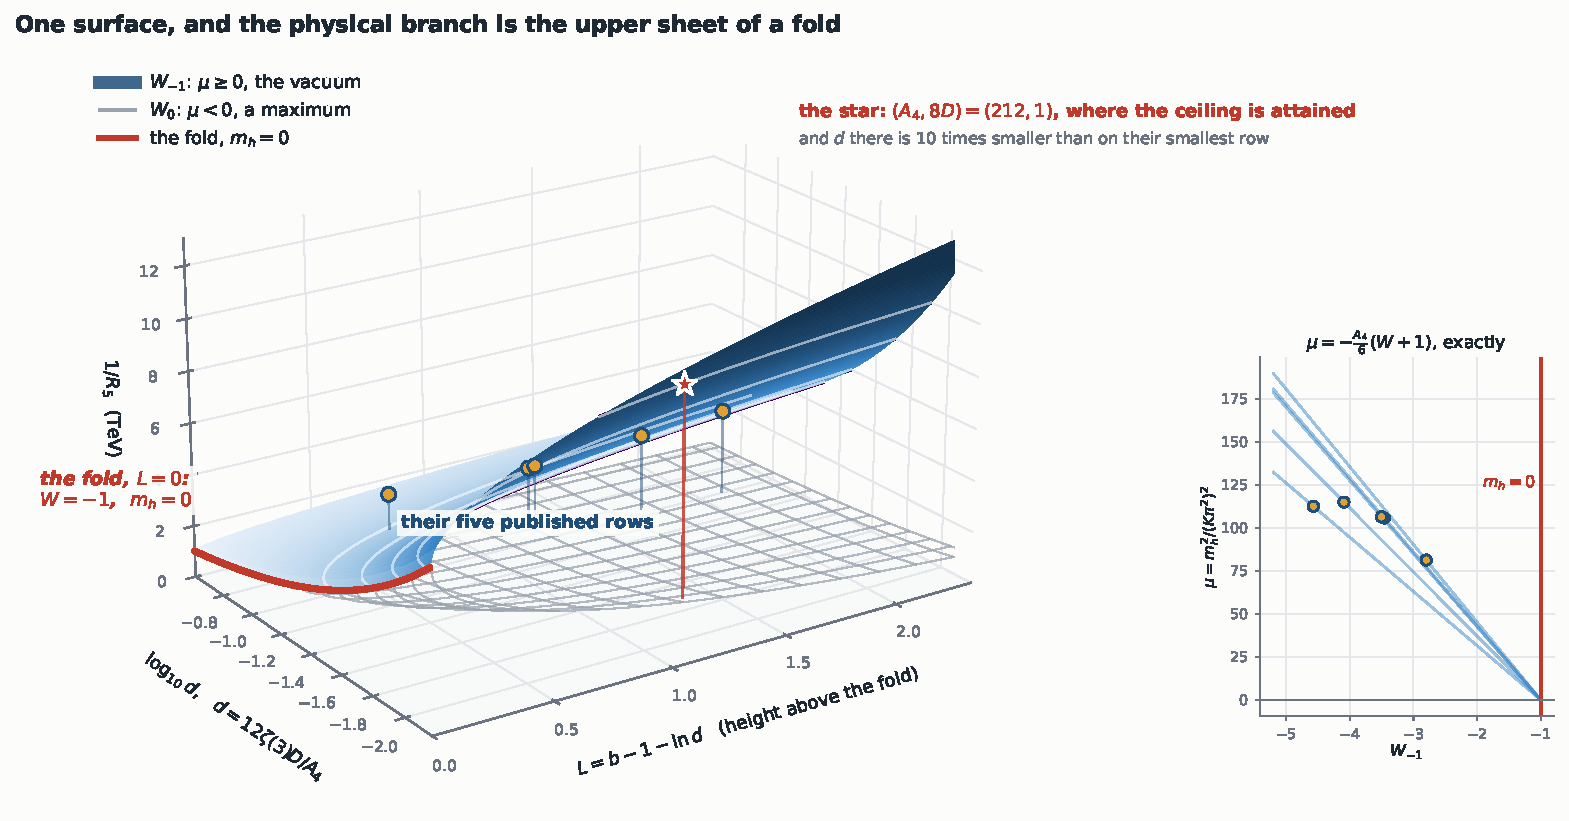
\includegraphics[width=\textwidth]{fig_lambert.pdf}
\caption{\textbf{The closed form is one sheet of a fold.} $1/R_5=2\pi m_W/x$ over the two
coordinates of \eqref{eq:foldsep}: $L=b-1-\ln d$, the discriminant, and $d=12\zeta(3)D/A_4$, on a
logarithmic axis because the certificate's vertex and their published rows differ by a factor of
ten in it. The blue sheet is $W_{-1}$, where $\mu\ge0$ and the stationary point is the vacuum; the
open grey mesh below it is $W_0$, where $\mu<0$ and the same point is a maximum. They meet along the
red edge $L=0$, where $W=-1$ and therefore $m_h=0$: this is the \emph{Lambert} branch point, where
the electroweak minimum and the outer root coalesce, and not the $\alpha^4\ln\alpha$ one at the
origin that \S\ref{sec:parity} turns on --- it is the fold Theorem~\ref{thm:eighths} is careful not
to claim, drawn rather than described. Amber discs are \cite{KM25}'s five rows; the star is
$(A_4,8D)=(212,1)$, the vertex the ceiling is attained at. \textbf{The star is not at
$10.03$~TeV and should not be}: the surface returns each content's \emph{own} stationary point,
$9967$~GeV there, while the certificate reads \eqref{eq:two}(II) at the top of the Higgs window
instead --- a $0.7\,\%$ difference, and the whole of it is which $m_h$ is being asked for.
\emph{Inset:} \eqref{eq:branchmu} as the straight line it is, one line per row, all five meeting at
$W=-1$, $\mu=0$. Drawn by \texttt{make\_\allowbreak fig\_\allowbreak lambert.py}, which refuses to
draw unless the surface returns every plotted $\amin$ --- it does, to
$2\times10^{-14}$.}\label{fig:lambert}
\end{figure}

\paragraph{Verification, against our own minimisation and not against their column.} What is tested
here is the expansion, not the anchor: a disagreement would be a defect of \eqref{eq:amin} and of
nothing else. Over $272$ synthetic contents spanning twelve values of $D$ and
$\amin\in[0.018,0.119]$ --- the range of their Table~1 --- the median error is $0.13\,\%$, and
$0.004\,\%$ at the small-$\alpha$ end where the truncated tail is smallest. On the five
published rows:

\begin{center}\small
\rowcolors{2}{white}{softgrey}
\begin{tabular}{lrrrrr}
\toprule
\rowcolor{hdrblue!10}row & $D$ & $A_4$ & numerical $\amin$ & closed form & error\\
\midrule
(1) & $15/8$ & $258$ & $0.055304$ & $0.055423$ & $0.215\,\%$\\
\rowcolor{amber!12}(2) & $29/8$ & $271$ & $0.083062$ & $0.083579$ & $0.623\,\%$\\
(3) & $9/8$  & $189$ & $0.043593$ & $0.043621$ & $0.065\,\%$\\
(4) & $11/8$ & $223$ & $0.046879$ & $0.046929$ & $0.107\,\%$\\
(5) & $15/8$ & $255$ & $0.055277$ & $0.055393$ & $0.209\,\%$\\
\bottomrule
\end{tabular}
\end{center}

\noindent Median $0.209\,\%$, maximum $0.623\,\%$ --- and the maximum falls on the row with the
largest $\alpha$, which is where the truncated tail is largest. Both are well
inside the two significant figures to which that table is printed.

Three controls run alongside, and the last is the one that could have failed. The $D$ column comes
out in exact eighths. The published ratio pattern of Part~VI \S7 is reproduced: $1.939$ on the two
rows with a $\rep{48}$ against $1.199$ on the other three. And \emph{dropping the logarithm} ---
using $x^2=24\zeta(3)D/4G$, which is what one would write without \S\ref{sec:parity} --- fails by
$+104$ to $+174\,\%$. The branch point is not a decoration.

\paragraph{And the truncation is a tail, not an asymptotic estimate --- which is a stronger
statement than it looks, and it is what \S\ref{sec:ceiling} will need.} The ladder does not stop at $p=1$. Its index continues to
$p=-1,-3,-5,\dots$, where $\zeta$ is \emph{rational} by Bernoulli, so past its own pole the
expansion generates no further transcendentals: the rung at order $x^{2k}$ is
$\zeta(5-2k)\,[\,A_{2k}+(2^{2k-4}-1)B_{2k}\,]$, which is \eqref{eq:ladderab} read at negative $p$,
and the antiperiodic weight runs $3,\,15,\,63,\,255,\dots=2^{2k-4}-1$. \textbf{There is exactly one
logarithm in the whole expansion}, at order $x^4$, and every term beyond it is rational in the
moments; the transcendental content of the potential is $\zeta(5)$, $\zeta(3)$, $\ln x$, $\ln 2$
and $\ln 3$, and nothing else. This is the classical expansion of $\mathrm{Li}_n(e^{\mu})$ about
$\mu=0$ \cite{Lewin}, valid for $|\mu|<2\pi$, and its $H_{n-1}-\ln(-\mu)$ term at $n=5$ is the
$H_4=\tfrac{25}{12}$ already carried by $G$ in \eqref{eq:moments} --- the same constant, arriving
by a second route. Once that single logarithm is extracted the remainder is therefore
the tail of a \emph{convergent} series, with radius fixed by the nearest singularity of
$\mathrm{Li}_5(s\,e^{ic\pi\alpha})$, at $s\,e^{ic\pi\alpha}=1$: $\alpha=2n/c$ for the periodic
tower and $\alpha=(2n+1)/c$ for the antiperiodic one, so $|\alpha|<1/c_{\max}=1/3$ covers both.
Measured term by term, the asymptotic ratio is $(c\alpha)^2$ antiperiodic and $(c\alpha/2)^2$
periodic, with controls on both sides of both radii --- the series is convergent at
$\alpha=0.32$ and divergent at $\alpha=0.40$ for the antiperiodic tower, and at $\alpha=0.40$ and
$\alpha=0.70$ for the periodic one. Every $\alpha$ this paper uses is inside $1/3$ by a factor of
at least $2.7$. \textbf{So the error committed here is a convergent remainder and admits a rigorous
bound rather than an estimate}, which is what the companion bound of
\texttt{remainder\_\allowbreak theorem.py} supplies. Measured in
\texttt{crossed\_\allowbreak equations.py}.

That the transcendental content is exactly $\{\zeta(5),\zeta(3),\ln x,\ln 2,\ln 3\}$ is not a
curiosity in passing; it is a coordinate system, and \S\ref{sec:ceiling} spends it. Because the only
logarithms of \emph{numbers} are $\ln2$ and $\ln3$ --- charges run to three and no further --- the
moment $G$ decomposes exactly in the basis $\{1,\ln2,\ln3\}$, which turns the transcendental
condition that decides the ceiling into an integer program. The two statements are one, read at
different rungs of the same ladder.

\bridge{The same expansion has a second output, and it is the column one does not expect for free.}

% ===================================================================
\section{The Higgs mass, from the same two moments}\label{sec:mh}

Differentiating \eqref{eq:Fexp} twice and using the stationarity condition to eliminate
$G-A_4\ln x$ produces a cancellation worth isolating:
\begin{keyeq}
\begin{equation}\label{eq:fpp}
  F''(\amin)\;=\;\pi^2\Bigl[\,2\zeta(3)D-\tfrac16 A_4 x^2\,\Bigr]\,.
\end{equation}
\textbf{The logarithm and $G$ cancel identically at the stationary point.}
\end{keyeq}

\noindent With their eq.~(80), $m_h=K\sqrt{F''(\amin)}/\amin$ and $K=(\sqrt3/2\pi^3)m_W g_4$, both
columns of their Table~1 are functions of $(D,A_4)$ alone, with no minimisation anywhere --- and
they return \emph{our} values of the two, since by \S\ref{sec:setting} the $\amin$ one does not
reproduce theirs. Against a
numerical second derivative of the same potential the closed form agrees to $0.13$--$1.22\,\%$
across the five rows, and the resulting $m_h$ to $0.07$--$0.61\,\%$.

A control that must fire, and does: their eq.~(80) returns no real $m_h$ where $F''<0$, and at
\emph{their} published $\alpha$ on row~(3) our assembly gives $F''=-2.45$. That is a symptom of the
anchor discrepancy of \S\ref{sec:setting}, recorded in Part~VI and not resolved here.

\bridge{Both observables now come from two integers in disguise. The next question is what those
integers are allowed to be.}

% ===================================================================
\section{The arithmetic of the content}\label{sec:arith}

In the sum/difference basis $S=A_2+B_2$, $\Delta=A_2-B_2$, the curvature rung reads
$8D=S+7\Delta$, and the seven is $2^3-1$ from the zeta ratio, not from $\su7$.

\paragraph{And that is not a coincidence of notation: $D$ \emph{is} a rung.} Writing the rung of
\S\ref{sec:ladder} as $O_k=[S_k+(2^p-1)\Delta_k]/2^p$ with $p=5-2k$ and reading it at the two values
of $k$ that this paper uses,
\[
  k=1:\quad O_1=\frac{S+7\Delta}{8}=D,
  \qquad\qquad
  k=0:\quad O_0=\frac{S_0+31\Delta_0}{32},\quad F(0)=\zeta(5)\,O_0 .
\]
So the curvature invariant of this section and the stability criterion of \cite{CCD24} are the same
object evaluated at two rungs of one ladder, and the $7$ and the $31$ are $2^p-1$ in each. The odd
eighths of Theorem~\ref{thm:eighths} and the bound $|F(0)|\ge\zeta(5)/32$ are then one statement read
twice, which is why the gauge sector's numerators $9$, $-27$, $-36$ at $k=0,1,2$ are odd, odd, even
\emph{on the seed \cite{KM25} print}: the obstruction is alive at the value and the curvature and
dies at the fourth moment, where $p=1$,
the antiperiodic half cancels to a finite $\ln2$ while the periodic pole survives as the
$x^4\ln x$. On the
candidate seed of \S\ref{sec:open} the same three numerators are $18$, $-18$, $-27$, and the
pattern \emph{permutes} to even, even, odd. What vanishes at $p=1$ is the antiperiodic half, not
the obstruction: it leaves the \emph{periodic} weight alone to carry the parity, and that weight
is exactly the one the fork of \S\ref{sec:open} turns on. \textbf{Read across the three rungs at
once, the ladder is a \emph{tomography} of the gauge seed}: at $p=5$ and $p=3$ the parity character
reads the two $P_6$ sectors in combination, and at $p=1$, where $2-2^{p}$ vanishes, it reads the
periodic sector alone. So moving the seed does not switch the protection off --- it moves it to the
rung that reads the half the seed changed.

\begin{theorem}[the odd eighths, conditional]\label{thm:eighths}
\emph{If} the gauge sector's contribution to $8D$ is odd, then $8D$ is an odd integer for every
bulk content. Hence $D\neq0$ and $|D|\ge\tfrac18$: \emph{the symmetric point} is never marginal at
one loop, and by a quantised amount.
\end{theorem}
\begin{keyeq}
\begin{equation}\label{eq:oddeighths}
  8D_{\mathrm{gauge}}\ \text{odd}
  \quad\Longrightarrow\quad 8D\in2\ZZ+1
  \quad\Longrightarrow\quad |D|\ \ge\ \tfrac18
\end{equation}
\end{keyeq}

\begin{corollary}[for the seed printed in \cite{KM25}]\label{cor:kmseed}
The gauge coefficients of \cite{KM25}'s eq.~(68) give $8D_{\mathrm{gauge}}=-27$, which is odd. The
hypothesis of Theorem~\ref{thm:eighths} is therefore satisfied, and every consequence drawn from it
below holds in this model.
\end{corollary}

\noindent \textbf{Why the hypothesis is separated out.} It is not a formality. The proof
needs two things: that matter contributes an even amount, and that the gauge sector contributes an
odd one. The first is arithmetic and cannot fail. The second is not computed here --- it is read
off someone else's equation, and \S\ref{sec:open} shows that reading is under active question.
Separating it costs nothing, since Corollary~\ref{cor:kmseed} restores every consequence verbatim
for the published seed. What it buys is the distinction that matters: \emph{if the seed moves, the
theorem stays true and its hypothesis stops being met}, which is a different situation entirely
from a theorem that fails. A conditional statement also says something the unconditional one
cannot --- exactly which downstream number is hostage to which upstream input.

\noindent \textbf{And only the symmetric point.} $D$ is the coefficient of $\alpha^2$ at
$\alpha=0$, so what is bounded away from zero is the curvature there. Whether the \emph{broken}
vacuum can be marginal --- $F''(\alpha_\star)=0$ at $\alpha_\star\neq0$ --- is a different
condition, and $D\neq0$ does not touch it. In the closed form of \S\ref{sec:closed} it is the
Lambert fold $W=-1$, equivalently $m_h=0$; it sits at $\alpha$ several times larger than any used
here, where the expansion's error scales up by the square of that ratio and, a fold being a
coalescence of roots, the position is in any case not controlled by a truncation. This paper
therefore neither asserts nor excludes it. Measured in
\texttt{lambert\_\allowbreak criticality.py}.
\begin{proof}
For matter, $c$ and $m$ are integers, so $S+\Delta=2A_2$ is even and $S+7\Delta=(S+\Delta)+6\Delta$
is even --- for \emph{every} content, with no reference to the gauge sector. By hypothesis the
gauge sector contributes an odd amount. Even plus odd is odd. For
Corollary~\ref{cor:kmseed}, the coefficients of \cite{KM25}'s eq.~(68) give
$S+7\Delta=-27$.
\end{proof}

\noindent The obstruction sits in the one row of the gauge table that mixes the two $P_6$ sectors
--- the $-\tfrac72$ of the $P_6=-1$ entry, reconstructed from their eqs.~(63)--(67) rather than
derived from the geometry (\S\ref{sec:open}). \textbf{And what carries the parity is the whole
coefficient of that row, not either weight inside it.} Written over its $n_+=2$ periodic and
$n_-=6$ antiperiodic pairs the row is $2a+6b$, which is $2\times2+6\times\tfrac12=7$ on the seed
\cite{KM25} print. The per-pair $\tfrac12$ does not do it alone: $6\times\tfrac12=3$ is an
\emph{integer}. What is odd is the \emph{sum}, and that needs the periodic part even just as much
as it needs the antiperiodic part odd --- which is the parity character \eqref{eq:chigauge} of the
affine gauge base point, and \S\ref{sec:open} is where that becomes the object the whole fork turns
on. A census over all
$4096$ admissible diagonal parity assignments gives the same statement in group-theoretic form:
$D$ can never vanish precisely when the block left unbroken by both projections has odd dimension,
and in their assignment that block is $\su3_C$. \emph{On the seed \cite{KM25} print, $D\neq0$
because the number of colours is odd} --- and that reading is a property of the weights
$(2,\tfrac12)$ and not of the group: at $(\tfrac32,\tfrac12)$ the same three colours are still
there, the census still returns the same count, and $8D$ is even all the same (\S\ref{sec:open}).
Within the five-dimensional $\su{N}$, $S^1/\ZZ_2$, single-Wilson-phase class \cite{HY04}'s formula
covers, no odd rung occurs; the second independent parity of this product orbifold is what supplies
the extra affine character that \emph{can} make one odd. Which parity the base point then lands on
is \eqref{eq:chigauge}.

\paragraph{The theorem has a dimension, and the obvious reason is not the right one.} In the
single-parity corner of \S\ref{sec:anchor} every tower is integer-moded, $B=0$, and $8D=8A_2$
is even; it would be easy to stop there. But a five-dimensional model on $S^1/\ZZ_2$ need not sit in
that corner --- with an antiperiodic sector $B\neq0$ --- and $8D$ is even there too, so
$B=0$ is not what is doing the work. Running Haba and
Yamashita's general five-dimensional formula \cite{HY04} over every boundary condition of
$\su{N}$ on $S^1/Z_2$ carrying a single Wilson phase, up to $N=12$, returns no odd $8D$ at all. The
mechanism is the counting of degrees of freedom: a Dirac fermion enters with $4$ and a complex
scalar with $-2$, both even, and the one odd coefficient --- the $-3$ of the gauge and ghost sector
--- multiplies only the adjoint, whose weight reaches $8D$ as $-24(2+\delta_1)+18\delta_2$ with
$\delta_1,\delta_2$ the block leftovers of their eq.~(5.9). Here the gauge sector instead delivers
the half-integer $-\tfrac72$ of their eq.~(68), and $6\times\tfrac72=21$ is odd. On Haba and
Yamashita's own $\su3$ example three multiplets suffice to lose the protection: one adjoint Dirac
fermion with $\eta\eta'=+$ and two fundamental ones with $\eta\eta'=-$ give $A_2=3$, $B_2=4$ and
$8D=0$ exactly. Marginality is not a fine-tuned corner in five dimensions; it is ordinary. What
forbids it here is the sixth dimension \emph{together with the gauge seed} \cite{KM25} print: the
candidate seed of \S\ref{sec:open} is equally six-dimensional, has the same three colours, and
reaches $8D=0$ on the lattice. The second parity supplies the extra affine character; which coset
the offset then lands in is a separate question, and it is the open one.

\begin{theorem}[a congruence mod six]\label{thm:mod6}
For every bulk content, $8D\equiv 2A_4+3 \pmod 6$.
\end{theorem}
\begin{keyeq}
\begin{equation}\label{eq:mod6law}
  8D\;\equiv\;2A_4+3 \pmod 6\qquad
  \text{\small for every bulk content, and on \emph{either} gauge seed}
\end{equation}
\end{keyeq}
\begin{proof}
Work with the single combination $8D-2A_4$, and separate the content from the gauge sector, which
enters only as a fixed base point. \emph{Matter:} a state with $s=-1$ contributes $-6mc^2$ to $8D$
and nothing to $A_4$, so $8D-2A_4$ receives $-6mc^2\equiv0\pmod6$; a state with $s=+1$ contributes
$8mc^2$ and $mc^4$, so it receives $8mc^2-2mc^4=2mc^2(4-c^2)$, which is even, and divisible by
three because $c^4\equiv c^2\pmod3$ for every integer $c$. Hence every bulk multiplet has
$8D-2A_4\equiv0\pmod 6$, and the eight generators confirm it one by one.
\emph{Gauge:} the coefficients \cite{KM25} print give $8D-2A_4=-27-2(-18)=9\equiv3\pmod6$. Adding
the two, $8D-2A_4\equiv3\pmod 6$ for every content.
\end{proof}

\noindent \textbf{Note that the proof never mentions a parity, and that is not a stylistic
preference.} An earlier version closed with ``modulo two the statement is
Theorem~\ref{thm:eighths}'', which is true for the published seed but makes a congruence about the
lattice depend on a theorem about one gauge offset. The argument above does not: the matter
sublattice is what it is, and the gauge sector enters only through the residue of $8D-2A_4$ at its
base point. That matters because the candidate seed of \S\ref{sec:open} gives
$-18-2(-\tfrac{27}{2})=9$ --- \emph{the same $9$} --- so Theorem~\ref{thm:mod6} holds unchanged on
either branch, \textbf{while the hypothesis of Theorem~\ref{thm:eighths} is not satisfied on the
candidate branch} --- the theorem itself is as true there as here. \emph{The mod-six law is the
general statement; the odd-eighth conclusion of Corollary~\ref{cor:kmseed} followed from it under
``$A_4$ integral'', and it is $A_4$ turning
half-integral that flips $2A_4+3$ from odd to even.} Which of the two is the deeper result is
not a matter of taste: one survives the change of hypothesis and the other does not.

\noindent The mod-three
half removes two thirds of the $(A_4,8D)$ plane and is what makes the certificate of
\S\ref{sec:ceiling} a statement about \emph{contents} rather than about a relaxation. Their five
published rows give $8D+A_4=273,300,198,234,270$, all divisible by three. That divisibility is not
a coincidence of the five and not the end of the statement: it is \eqref{eq:congr5} read modulo
three, and the same congruence holds modulo \emph{nine} once $2U$ is carried along.

\paragraph{And the same argument one rung up --- in fact at every rung at once.} Split the table
into its periodic and antiperiodic halves. \textbf{The subscript here is the \emph{rung}, not
the power}, so write them calligraphically to keep them apart from the moments of
\eqref{eq:moments}: $\mathcal{A}_k=\sum_{s=+}mc^{2k}$ and $\mathcal{B}_k=\sum_{s=-}mc^{2k}$, so that
$\mathcal{A}_1=A_2$ and $\mathcal{A}_2=A_4$. \textbf{And $\mathcal{B}_k$ is not the per-pair weight $b$}: $b$ weighs
one $P_6=-1$ pair, while $\mathcal{B}_k$ is the whole $s=-1$ sector summed over \emph{both} $P_6$
classes, so the periodic weight $a$ sits inside it. That is why $\mathcal{B}_k$ moves from $-\tfrac72$
to $-3$ between the two seeds of \S\ref{sec:open} while $b=\tfrac12$ does not move at all; the two
letters are close enough to be worth separating once, here. Then $S_k=\mathcal{A}_k+\mathcal{B}_k$, $\Delta_k=\mathcal{A}_k-\mathcal{B}_k$, and the whole
ladder collapses to
\begin{keyeq}
\begin{equation}\label{eq:ladderab}
  2^{p}O_k \;=\; 2^{p}\mathcal{A}_k \;+\; \bigl(2-2^{p}\bigr)\mathcal{B}_k , \qquad p=5-2k .
\end{equation}
\end{keyeq}
For the gauge sector on the seed \cite{KM25} print, $\mathcal{A}_k=-4^k-2$ and
$\mathcal{B}_k=-\tfrac72$, and since $2^{p}4^{k}=2^{5}$ the $k$
cancels, leaving one number for the whole ladder:
\begin{keyeq}
\begin{equation}\label{eq:gaugerung}
  2^{p}O_k^{\,\text{gauge}} \;=\; -39 + 3\cdot 2^{\,p-1}
  \qquad\longrightarrow\qquad 9,\;-27,\;-36 \quad\text{at } k=0,1,2 .
\end{equation}
\end{keyeq}
Equation \eqref{eq:gaugerung} is \S\ref{sec:ladder}'s two-parameter ladder written out: since
$2^{\,p-1}=16\cdot4^{-k}$, it reads $-39\cdot1^{k}+48\cdot(\tfrac14)^{k}$, which are exactly the two
modes $\sigma\in\{1,\tfrac14\}$ the gauge sector was found to reach --- now with their amplitudes,
$-39$ and $48$. The identity $O(5)-O(3)=4[O(3)-O(1)]$ is then not a coincidence to be checked but an
algebraic consequence: for any $O_k=A+B(\tfrac14)^k$ the two sides are $3B/4$ and $3B/16$.

Matter has integer $m$ and $c$, and at the three rungs of integer normalisation, $p=5,3,1$, both
coefficients in \eqref{eq:ladderab} are even --- $32$ and $-30$, $8$ and $-6$, $2$ and $0$ --- so
matter contributes an even integer to $2^{p}O_k$ on each. Past the pole, at $p=-1,-3,\dots$, those
coefficients are fractional and the \emph{arithmetic} ladder has no rung to stand on, though the
analytic one continues. On the three:
\textbf{whatever parity a rung has is the gauge sector's alone}, and what decides it is the
parity character \eqref{eq:chigauge} of the complete gauge coefficient --- on the seed \cite{KM25}
print, $\mathcal{B}_k$ half-integral is what makes that character odd, and \S\ref{sec:open} is where
the character itself becomes the object. That is a statement about the two parity-sensitive rungs
and no others: at $p=1$ the antiperiodic weight $2-2^{p}$ vanishes identically, $\mathcal{B}_k$
drops out, and the fourth-moment rung is left to the \emph{periodic} gauge weight alone --- which
is the weight \S\ref{sec:open} puts in question. It is even on the seed \cite{KM25} print, where
the obstruction dies at that rung, and \emph{odd} on the candidate seed, where that rung is the
one the obstruction survives on. At $k=0$ that gives $32F(0)/\zeta(5)$ always odd and
\begin{keyeq}
\begin{equation}\label{eq:valuebound}
  |F(0)|\;\ge\;\frac{\zeta(5)}{32}\qquad
  \text{\small for every bulk content, and attained --- on the seed \cite{KM25} print}
\end{equation}
\end{keyeq}
The zeta value is inherited, not derived here. \cite{HHHK03} evaluate the Wilson-line potential at
these special points and get $f_D(0)=\zeta_R(D)$ and $F=\sum(2n-1)^{-5}=(1-2^{-5})\zeta_R(5)$: that
$\tfrac{31}{32}$ is ours only in the sense that we read it from them, and the $\zeta(3)$ one rung up
is the same inheritance. The claim is the coefficient in front. It is quantised, so the value
cannot be made small by any choice of content. Like the odd eighths it rests on $\mathcal{B}_k$ being
a half-integer --- which is the \emph{same} statement as the parity character of the whole mixed
row and not a rival to it, a distinction worth making because the row is where the two readings of
\S\ref{sec:open} differ. $\mathcal{B}_k$ is $-(2a+6b)/2$, so the \emph{periodic} weight $a$ sits
inside it: it moves from $-\tfrac72$ to $-3$ on the candidate seed, while the per-pair
$b=\tfrac12$ does not move at all. What is not the reason is $b$ on its own.

In the language of \cite{CCD24}, whose stability criterion \emph{is} this rung, the comparison of
the symmetric point against the maximal one, applied to a model they did not consider, is never a
tie. And \eqref{eq:ladderab} says why the obstruction dies at $k=2$ on the seed \cite{KM25} print,
which is otherwise only an
observation about the number $-36$: the antiperiodic half enters with $2-2^{p}$, and at $p=1$ that
is \emph{exactly zero}. The fourth moment does not see the antiperiodic sector at all --- $2O_2=2\mathcal{A}_2=2A_4$,
and the half-integer never enters, which is why the parity left at that rung is the periodic
weight's and travels with the seed. That is also why $A_4$, the entire non-analyticity, is the one
thing matter \emph{can} cancel: at that rung there is only a periodic sum to cancel. Seventeen
contents of at most six multiplets have $A_4=0$ exactly, five of them with $D>0$.

\paragraph{And cancelling it is not free: the analytic branch is charged twice over.} $A_4=0$ is
the one place where the vacuum becomes analytic at the symmetric point, so it is worth asking what
such a content can do. Theorem~\ref{thm:mod6} answers before any dynamics does: $8D\equiv 2A_4+3
\pmod 6$ forces $8D\equiv3\pmod6$ when $A_4=0$, so $8D\in\{3,9,15,\dots\}$ and \textbf{$8D=1$ is
arithmetically forbidden} --- and $8D=1$ is exactly the quantum on which the ceiling of
\S\ref{sec:ceiling} sits. Maximal hierarchy and maximal analyticity are incompatible, and what
makes them so is a congruence rather than a mechanism. The smallest $8D$ actually realised with
$A_4=0$ and $D>0$ is $15$, not $3$.

There is a second charge behind the first, and unlike the congruence it can be settled
\emph{exhaustively}, because the branch is finite in the only direction that matters. Exactly one
multiplet has $A_4=0$, the $\rep7^{(+,+)}$, so it may be added freely without leaving the branch
while every other multiplet has $A_4>0$ and must therefore make up the gauge sector's $-18$ exactly
--- which admits eleven solutions and no more. The free multiplet is then the only knob, and it
moves the two functionals that matter at a fixed rate: $8D\to8D-6n$ and $W\to W+n$, six units of
curvature bought for one of stability. Electroweak breaking asks $n<8D_{\text{base}}/6$ and a true
vacuum asks $n>-W_{\text{base}}$, so both together need an integer in an interval, and over the
eleven base solutions there is none:
\begin{keyeq}
\begin{equation}\label{eq:analytic}
  A_4=0\;\Longrightarrow\;\text{no content has both } D>0 \text{ and } W>0 .
\end{equation}
\end{keyeq}
\noindent \textbf{Cancelling the branch point, breaking the electroweak symmetry and landing in the
true vacuum cannot be done at once.} And it is close: the widest window is $18\times\rep7^{(+,-)}$,
with $8D=117$ and $W=-\tfrac{39}{2}$, where $n=19$ gives $8D=3>0$ but $W=-\tfrac12<0$, and $n=20$
gives $W=\tfrac12>0$ but $8D=-3<0$. One step of the only knob there is. The statement is exact
arithmetic on two integers --- no expansion enters, which matters here because the closed form has
no business on this branch at all: its champion sits at $\alpha=2m_W/181\simeq0.89$, a factor $2.7$
\emph{outside} the radius $1/3$ that \S\ref{sec:closed} proves. \textbf{An earlier version of this
paper quoted $m_h\le29.6$~GeV here; that number was computed outside the radius and is withdrawn.}
The exact potential agrees with \eqref{eq:analytic}: every base family with $D>0$ has no global
interior minimum at all. Measured in \texttt{analytic\_\allowbreak branch\_\allowbreak nogo.py} and
\texttt{analytic\_\allowbreak branch\_\allowbreak exact.py}; the enumeration of the seventeen is
\texttt{moment\_\allowbreak ladder.py}.

All of \S\ref{sec:arith} is arithmetic of the content, and Figure~\ref{fig:collapse} is what it
looks like from the outside: the same $4319$ contents plotted against their own size, against the
two observables they produce, and against the precision a measurement would need to tell them
apart.

\begin{figure}[t]
\centering
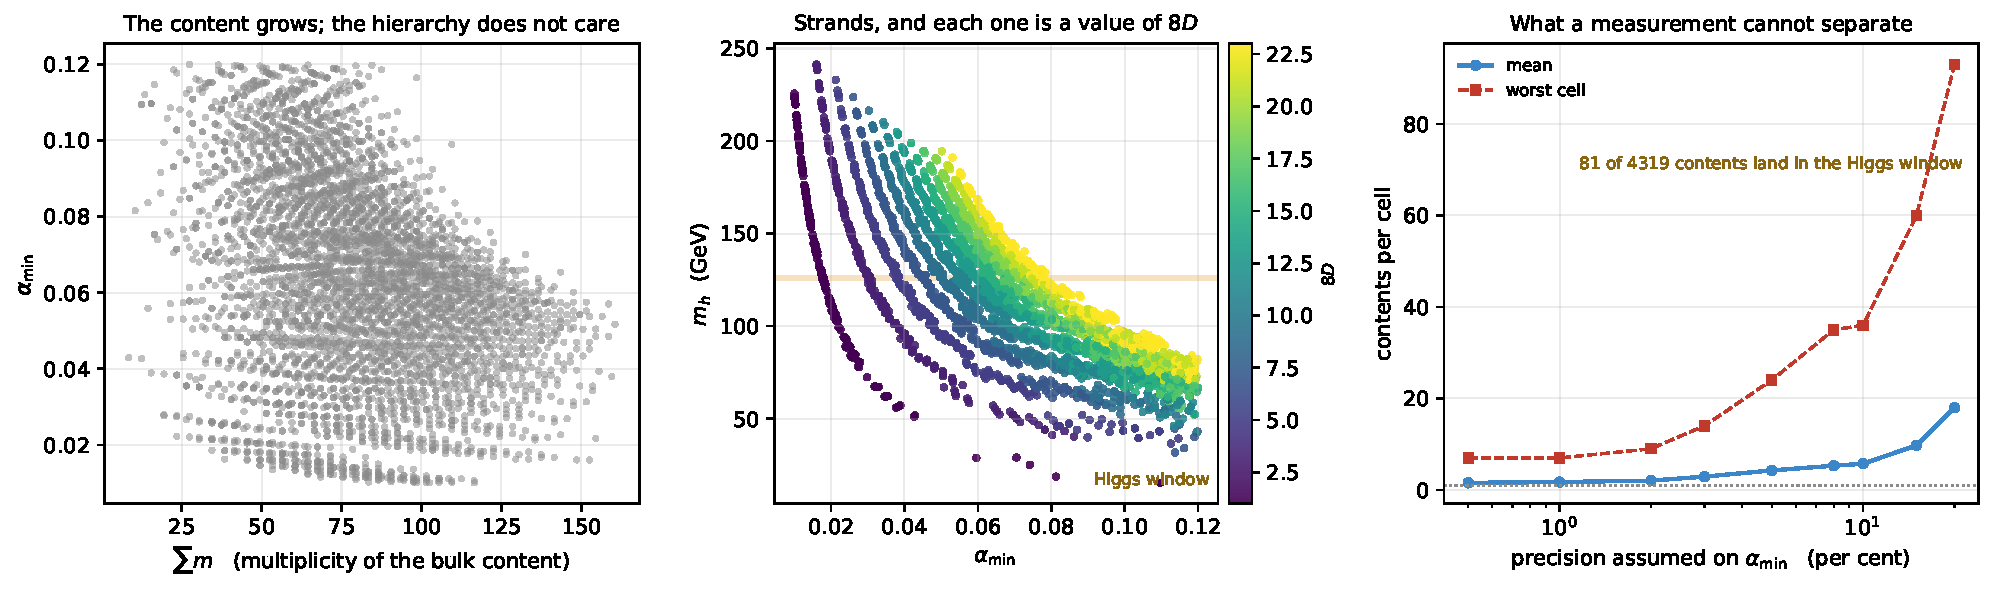
\includegraphics[width=\textwidth]{fig_collapse_lattice.pdf}
\caption{\textbf{The arithmetic, seen from the observable side.} Every content built from at most
four copies of each of the eight multiplets, kept when $0<D\le3$ and $\amin\in[0.010,0.120]$:
$4319$ of them. \emph{Left:} $\amin$ against the total multiplicity of the bulk content. There is
no relation --- the hierarchy does not care how much matter there is, only how it is distributed
over charge and parity. \emph{Centre:} the same contents in the plane of the two observables they
predict. The cloud separates into strands, and each strand is one value of $8D$; the Higgs window
crosses them, so which contents are viable is a question about the second moment rather than about
the size of the model. Coloured by multiplicity instead, the same panel shows nothing.
\emph{Right:} how many contents share one cell of the observable plane, against the precision
assumed on $\amin$ --- with the $m_h$ side of the cell relaxed alongside it, from $1$ to $5$~GeV,
because a measurement that loosens one loosens the other. At the finest cell drawn the mean is
$1.55$ and the worst cell holds $7$; at the loosest, $20\,\%$ in $\amin$ and $5$~GeV in $m_h$, the
mean is $18.0$ and the worst cell holds $93$. The two observables therefore determine the content only to the extent that they are
measured well, and the quantisation of \S\ref{sec:arith} is what sets the scale of that trade.
$81$ of the $4319$ land inside $125$--$127$~GeV.}\label{fig:collapse}
\end{figure}

\bridge{Two quantised moments, one universal kernel, and a hierarchy that is their ratio. What is
the largest hierarchy the lattice allows?}

% ===================================================================
\section{The ceiling}\label{sec:ceiling}

\paragraph{First, two identities with no logarithm in them.} Write
$\mu = m_h^2/(K\pi^2)^2$ --- the Higgs mass in the units the potential works in. Eliminating the
logarithm between \eqref{eq:fpp} and the fixed point \eqref{eq:amin} leaves
\begin{keyeq}
\begin{equation}\label{eq:two}
  \text{(I)}\quad \ln x \;=\; \frac{G-3\mu}{A_4}-\frac34\,,
  \qquad\qquad
  \text{(II)}\quad x^2 \;=\; \frac{12\,\zeta(3)\,D}{6\mu+A_4}\,.
\end{equation}
\end{keyeq}
\noindent Both are verified to $6\times10^{-14}$ on the five published rows --- and that number
should be read for what it is. (I) and (II) are obtained \emph{algebraically} from
\eqref{eq:fpp} and \eqref{eq:amin}, so $6\times10^{-14}$ tests the implementation and the algebra
and nothing else: an identity derived from a truncated expansion verifies to machine precision
while inheriting every bit of the truncation error of its parents. The physical validation is a
different measurement and it is the one in \S\ref{sec:closed}: $0.13\,\%$ median and $0.62\,\%$
worst against numerical minimisation of the untruncated potential. Internal exactness and external
accuracy are separate claims and are kept separate here. (II) is the useful one:
\emph{once the Higgs mass is pinned, $\amin$ is algebraic in the two moments} --- no fixed point, no
logarithm. Since $1/R_5=2\pi m_W/x$, maximising the compactification scale means making $D$ small
and $A_4$ large; and $D$ cannot go below $1/8$ by Theorem~\ref{thm:eighths}. So the ceiling is the
question of how far $A_4$ can be pushed before (I) runs out of contents that satisfy it.

\paragraph{That question is an integer program.} All three moments are \emph{linear} in the
multiplicity vector $n\in\ZZ_{\ge0}^8$, and $A_4$ and $8D$ are integers. For a content at
$(A_4,8D)=(t,k)$ whose Higgs mass sits at the top of the window, (II) fixes $x$ with no freedom
left, and (I) then demands a specific value of $G$:
\begin{equation}\label{eq:gstar}
  G^\star(t,k)\;=\;t\Bigl(\ln x+\tfrac34\Bigr)+3\mu\,,\qquad
  x=\sqrt{\frac{12\zeta(3)(k/8)}{6\mu+t}}\,,
\end{equation}
so the pair $(t,k)$ is realisable only if some content there has $G\le G^\star(t,k)$. Relaxing the
multiplicities to the reals turns ``the smallest $G$ at $(t,k)$'' into a linear program with two
equality constraints --- whose \emph{dual} therefore has two variables \cite{Schrijver}, so its
vertices can be enumerated exactly in rational arithmetic, with $\ln 2$ and $\ln 3$ rounded in the
direction that keeps the bound a bound. Admissible $(t,k)$ are restricted by Theorem~\ref{thm:mod6}, and the
restriction bites: the optimum of the relaxation falls at $(216,1)$, where $216+1$ is not divisible
by three, so no content sits there at all. Figure~\ref{fig:cone} is the lattice the program runs on,
and its right-hand panel is where the one-in-six comes from.

\begin{figure}[t]\centering
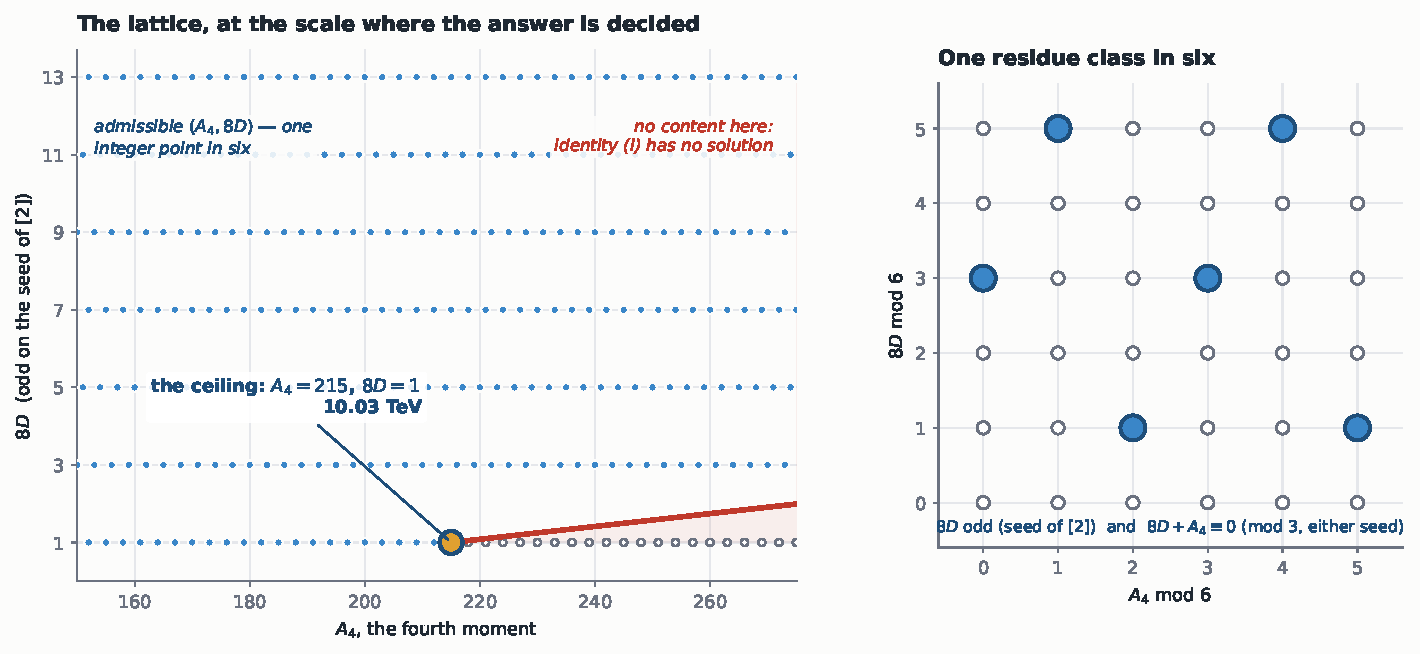
\includegraphics[width=\textwidth]{fig_cone.pdf}
\caption{\textbf{The lattice the integer program runs on.} Left, at the scale where the answer is decided: the admissible $(A_4,8D)$ are one integer point in six, the red curve is where identity (I) runs out of contents in the relaxation, and the hollow points beyond it are unrealisable. The relaxation's maximum sits on the last admissible point of the row $8D=1$ --- and Figure~\ref{fig:lift} shows that \emph{that} point is empty once the third coordinate is counted, so the integer maximum is the one below it. Right: why one in six --- $8D$ odd on the seed \cite{KM25} print, which is Corollary~\ref{cor:kmseed}, together with $8D+A_4\equiv0\pmod3$, which is Theorem~\ref{thm:mod6} on either seed. The geometry is computed exactly in Sage: the cone has extreme rays $(0,-1)$ and $(1,8)$, dual description $\{A_4\ge0,\ 8D\le 8A_4\}$, and the eight multiplets generate a sublattice of index exactly $6$ in $\mathbb{Z}^2$ --- the congruence, restated as a lattice index. Its Hilbert basis is $\{(0,-1),(1,8)\}$, and $(0,-1)$ is \emph{not} reachable: the $\mathbf{7}^{(+,+)}$ steps down by six, never by one.}\label{fig:cone}
\end{figure}

\begin{keyeq}
\begin{equation}\label{eq:ceiling}
  \boxed{\;\frac{1}{R_5}\;\le\;10.03\ \text{TeV}\;}
  % \quad y no \qquad, para que las dos ediciones lleven el MISMO espaciado: al acortar la linea
  % castellana lo cambie solo alli y check_formulas lo caz'o como formula que difiere entre
  % ediciones, que es exactamente para lo que esta.
  \quad\text{certified at } A_4=215,\ D=\tfrac18 .
\end{equation}
\end{keyeq}

\noindent \textbf{And the quantifier deserves saying exactly.} The dual certifies each rung it is
run on, for arbitrary content \emph{on that rung}. Extending that to a maximum over \emph{all}
rungs uses one more thing: that $t^\star(k)/k$ is non-increasing. That was measured to $k=501$ for
two weeks and is now proved, in the paragraph after next.

\noindent The per-$D$ ceiling is monotone decreasing --- $10.03$, $6.27$, $4.21$, $3.14$, $2.80$~TeV
at $8D=1,3,9,33,129$ --- flattening towards about $2.7$~TeV. So the maximum sits \emph{on the
quantum} $D=1/8$: Part~VI observed that the eight contents of smallest $\amin$ all had $D=1/8$; here
that is not an observation about an enumeration but where the argument maximum is, and
Theorem~\ref{thm:eighths} is doing the physical work. That monotonicity is worth saying carefully,
because the whole ceiling rests on it. From (II), $(1/R_5)^2\propto(6\mu+t^\star(k))/k$ with
$t^\star(k)$ the largest admissible $A_4$ on rung $k$, so a \emph{sufficient} condition is that
$t^\star(k)/k$ be non-increasing --- and it is, falling from $215$ at $k=1$ through $70$ at $k=9$ to
$50.8$ at $k=501$, monotonically at every step. Measured in \texttt{fissures.py}.

\paragraph{And it is a sign, not a scan.} Since $1/R_5=2\pi m_W/x$ and (II) fixes $x$, the ceiling
depends on the rung \emph{only} through the slope $r_k=t^\star(k)/k$:
\begin{equation}\label{eq:slope}
  M(k)^2\;=\;\frac{8\pi^2m_W^2}{3\zeta(3)}\Bigl(r_k+\frac{6\mu}{k}\Bigr),
\end{equation}
so the question is a derivative of one function of one variable. Two facts settle it. First, the
dual of \S\ref{sec:ceiling}'s program has \textbf{exactly two vertices}, and \emph{one} of them is
active at every rung --- so the piecewise-affine argument has a single piece and there are no
boundaries to check. Second, writing $t=rk$ makes $x^2=(3\zeta(3)/2)/(r+6\mu/k)$, and the active
vertex's condition becomes $\Phi(r,k)\ge0$ with
$\Phi=r\bigl(A-\tfrac12\ln(r+6\mu/k)\bigr)-\nu-C/k$, $A=\tfrac12\ln\tfrac{3\zeta(3)}2+\tfrac34-\lambda$
and $C=G_{\text{gauge}}-\lambda A_{\text{gauge}}-\nu\,(8D)_{\text{gauge}}-3\mu$. Then
\begin{equation}\label{eq:dphidk}
  k^2\,\frac{\partial\Phi}{\partial k}\;=\;\frac{3\mu\,r}{r+6\mu/k}\;+\;C ,
\end{equation}
whose first term is positive and strictly below $3\mu$. So $\partial\Phi/\partial k<0$ as soon as
$C\le-3\mu$, which is the statement $G_{\text{gauge}}-\lambda A_{\text{gauge}}-\nu(8D)_{\text{gauge}}\le0$
--- \textbf{a condition on the gauge sector alone}, and it holds with room: $-37.43\le0$. With
$\partial\Phi/\partial r<0$ at the upper root, $dr^\star/dk<0$. Both terms of \eqref{eq:slope}
therefore fall, $M(k)$ strictly decreases, and since the integer ceiling never exceeds the real
relaxation, $M(k)\le M_{\text{real}}(3)=6268$~GeV for every $k\ge3$, below the $10\,034$~GeV of
$8D=1$. \textbf{The maximum sits on the quantum because it must.}

\paragraph{And the flattening has a value.} $\Phi$'s large-$k$ limit drops $k$ entirely and leaves
$r(A-\tfrac12\ln r)=\nu$, a Lambert equation whose two real branches are the ends of an interval of
admissible slopes: $r=-2\nu/W(-2\nu e^{-2A})$. Intersecting the two vertices' intervals,
\begin{equation}\label{eq:rinf}
  r_\infty=50.6809086439,\qquad
  M_\infty=\sqrt{\tfrac{8\pi^2m_W^2}{3\zeta(3)}\,r_\infty}=2\,678~\text{GeV},
\end{equation}
approached from above and never reached. So the $2.7$~TeV the table flattens towards is not a
numerical coincidence: it is the asymptotic ray of the feasible cone, and the ceiling runs from
$10.03$~TeV on the smallest rung --- on the seed \cite{KM25} print, since which rung is smallest is
what the seed decides --- to $2.678$~TeV at infinity. The asymptote itself is not conditional: it
carries no gauge quantity at all. Measured in
\texttt{asymptotic\_\allowbreak ray.py}.

\paragraph{A number of ours, corrected.} An earlier note of this series quoted $1/R_5\le2.18$~TeV
under the same Higgs window. That is a bound on the \emph{size} of the content --- it is what an
enumeration over contents of at most six multiplets returns, six being the size used in their
Table~1 --- and not a bound on the model, which does not cap the content at all. Opening the cap:

\begin{center}\small
\rowcolors{2}{white}{softgrey}
\begin{tabular}{crrcl}
\toprule
\rowcolor{hdrblue!10}$N$ & in window & best $1/R_5$ & $D$ & content\\
\midrule
$5$  & $1$    & $1924$ & $29/8$ & $\rep{28}^{++}+4\times\rep{84}^{++}$\\
$6$  & $3$    & $2182$ & $21/8$ & $\rep{28}^{++}+\rep{28}^{+-}+\rep{48}^{++}+3\times\rep{84}^{++}$\\
$7$  & $15$   & $3604$ & $7/8$  & $3\times\rep7^{++}+2\times\rep{28}^{++}+2\times\rep{84}^{++}$\\
\rowcolor{amber!14}$8$  & $30$   & $\mathbf{9138}$ & $\mathbf{1/8}$ & $3\times\rep7^{++}+\rep7^{+-}+2\times\rep{48}^{++}+\rep{48}^{+-}+\rep{84}^{++}$\\
$14$ & $1097$ & $9156$ & $1/8$  & $4\times\rep7^{++}+2\times\rep{28}^{++}+5\times\rep{28}^{+-}+\rep{84}^{++}$\\
\bottomrule
\end{tabular}
\end{center}

\noindent The jump is between seven and eight multiplets and is a factor of $2.5$: eight is where
the lattice first manages to sit on $D=1/8$ \emph{inside} the Higgs window. Two more multiplets than
their Table~1 uses, not seventy. Figure~\ref{fig:ceiling} plots both halves of the claim: the jump
against the cap on the content, and the ceiling's monotonicity in $D$.

\begin{figure}[t]\centering
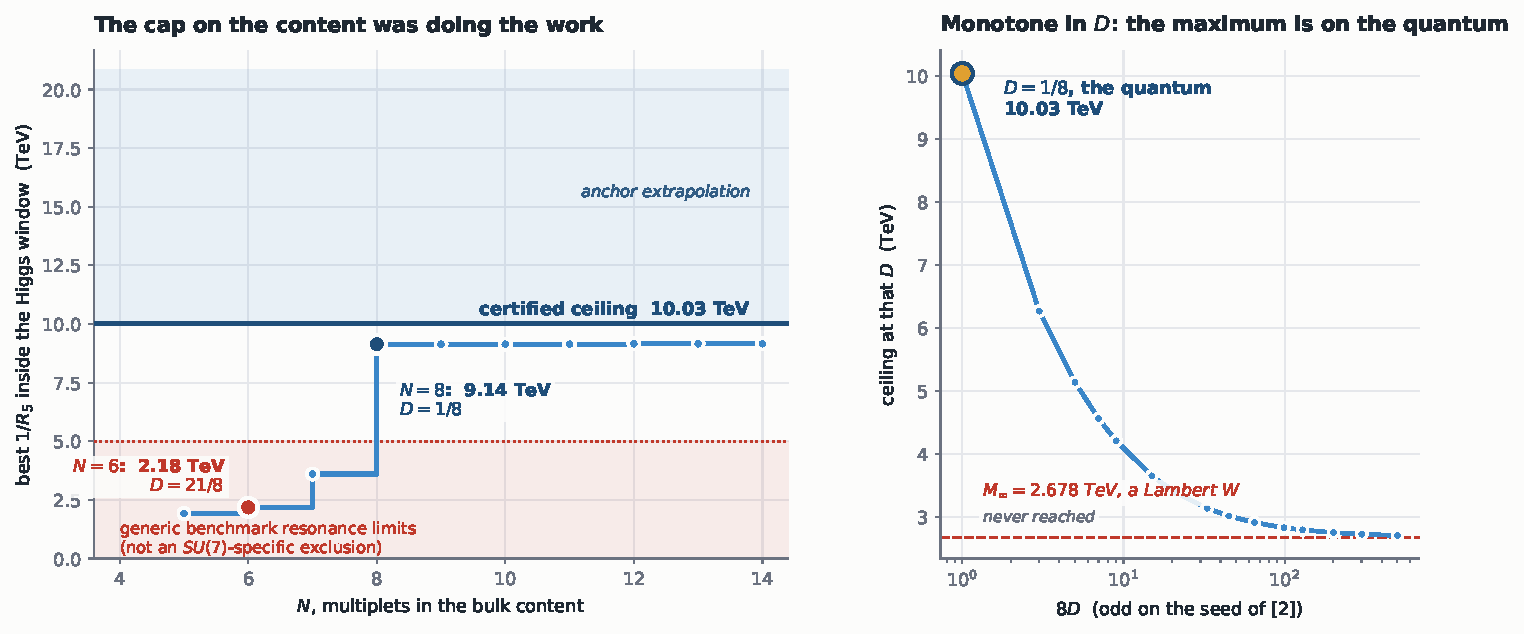
\includegraphics[width=\textwidth]{fig_ceiling.pdf}
\caption{\textbf{The cap on the content was doing the work.} Left: the best $1/R_5$ inside the Higgs window against the number of multiplets allowed. The $2.18$~TeV quoted earlier in this series is the $N=6$ point; at $N=8$ the lattice first reaches the quantum $D=1/8$ of the seed \cite{KM25} print and the scale jumps by a factor $2.5$. The horizontal line is the certified ceiling, the band above it the anchor \emph{extrapolation} of \S\ref{sec:setting} --- which \S\ref{sec:setting} is careful to say is a trend and not an uncertainty, and the figure labels the same way --- and the shaded region the reach of generic benchmark resonance searches --- \textbf{not an $\su7$-specific exclusion}: \S\ref{sec:collider} shows those limits are set on a \emph{narrow} resonance and cannot be carried to an object with $\Gamma/M\simeq0.16$ and an unfixed $\mathrm{BR}(G_1\to jj)$. Right: the ceiling as a function of $D$ --- monotone, so the maximum sits on the quantum, which is Theorem~\ref{thm:eighths} doing physical work.}\label{fig:ceiling}
\end{figure}

\paragraph{And that table is where the certificate stops being the answer.} The relaxation's
optimum sits at $(A_4,8D)=(215,1)$ and the enumeration climbs only to $9.16$~TeV. The dual bounds
the whole cone, and that is a theorem; whether an integer content \emph{sits} on the certifying
vertex is a further question, and it is decidable rather than open --- because in the right
coordinates the obstruction stops being transcendental.

Write $G$ exactly. The charges are $c\in\{1,2,3\}$, so $A_4^{L}$ and $B_4$ contribute only
$\ln 2$ and $\ln 3$, and
\begin{equation}\label{eq:UV}
  G\;=\;\tfrac{25}{12}A_4\;-\;U\ln 2\;-\;V\ln 3\,,
\end{equation}
with $U$ half-integer and $V$ integer, both linear in the multiplicities. Since $\ln2/\ln3$ is
irrational --- $2^q=3^p$ has no solution --- the pair $(U,V)$ is not lost inside $G$, and the
content lives on a \emph{four}-dimensional lattice $(A_4,8D,2U,V)$ rather than the two-dimensional
one of Figure~\ref{fig:cone}. It is worth being careful about the fourth coordinate, because there
is a tempting false step: $\ln3$ enters through the single generator $\rep{84}^{(+,-)}$, so
$V=81\,n_{\rep{84}^{(+,-)}}$ --- and that makes $V$ cheap to describe but \emph{does not} make it
dependent on the other three. The seven generators with $V=0$ already reach rank three in
$(A_4,8D,2U)$, so the eighth can only add a direction, and the rank is four.

The right object is then the finite group $\ZZ^r/L$, whose invariant factors are the congruences.
A Smith normal form gives
\begin{equation}\label{eq:snf}
  \ZZ^2/L\cong\ZZ_6\,,\qquad
  \ZZ^3/L\cong\ZZ_2\times\ZZ_{72}\,,\qquad
  \ZZ^4/L\cong\ZZ_{18}\times\ZZ_{648}\,,
\end{equation}
of orders $6$, $144$ and $11664$. So the projected law of Theorem~\ref{thm:mod6} is the single
congruence $\ZZ_6$, and the lifted content is \textbf{two} congruences and not one --- an index is
the order of a group, not a count of conditions, and the number of independent conditions is at most
the rank. Two earlier sections turn out to have been describing this lattice without naming it.
\S\ref{sec:closed} is what licenses the basis: the transcendental content of the whole potential is
$\{\zeta(5),\zeta(3),\ln x,\ln 2,\ln 3\}$ and nothing else, so $\{1,\ln2,\ln3\}$ is not a
convenient truncation but the complete span. And the log-free charge-two flip of
\S\ref{sec:ladder}, \eqref{eq:c2flip}, is exactly the direction with $\Delta U=\Delta V=0$: the one
generator move the third axis cannot see, which is why its $\Delta G$ was rational. Figure
\ref{fig:lift} is the two pictures side by side.

\paragraph{And lifting once more closes it, because the fifth coordinate is $2W$.} Carrying $W$ up
as a coordinate rather than a screen --- Figure~\ref{fig:lift} with one axis more --- gives
$(A_4,8D,2U,V,2W)$, integral in every entry once $U$ and
$W$ are doubled, of rank \emph{five}, with
\begin{equation}\label{eq:snf5}
  \ZZ^5/L\;\cong\;\ZZ_2\times\ZZ_{72}\times\ZZ_{2592},\qquad\text{index }373\,248 .
\end{equation}
Five is also the dimension of the function space of \S\ref{sec:closed}, and that is not a
coincidence:
\begin{theorem}[complete invariants]\label{thm:complete}
Two bulk contents have the same one-loop potential, as a function of $\alpha$, if and only if they
agree on $(A_4,8D,2U,V,2W)$.
\end{theorem}
\noindent The proof is two kernels meeting. Content $\mapsto$ potential has a three-dimensional
kernel, spanned by \eqref{eq:fivegen}; content $\mapsto$ the five coordinates has a
three-dimensional kernel because the rank is five; and the first is contained in the second because
each coordinate is a linear functional of the potential. Equal dimensions and one inside the other
make them equal. The two kernels are computed here by routes sharing no arithmetic --- one from the
Fourier vectors, one from the moment definitions --- and come out generator for generator the same.
Figure~\ref{fig:kernel} is the statement and its reason side by side.

\paragraph{What of that is not new, and one instance of it is in print.} That the potential is a
\emph{linear form in the bulk content}, with the gauge sector as a constant offset, is standard and
explicit: \cite{HY04} eq.~(3.20) writes exactly that and closes with ``this counting rule for the
coefficients of the effective potential is applicable in general'', and \cite{CCD24} eqs.~(2.7) and
(2.9) restate it. Degenerate contents therefore \emph{exist} as a matter of counting, and one is
printed: \cite{CCD24} eq.~(3.26) has two SU(6) models whose bulk fermions differ --- two
$\rep{15}$'s against $\rep6+\rep{\bar6}+\rep{20}$ --- and whose gauge-scalar potentials agree
identically, recorded as ``accidentally the same''. \textbf{That is an element of the kernel below,
and it is not an accident.} A second sits unremarked in the equations of the five-dimensional
ancestor of this model: \cite{KTY17} eqs.~(3.10)--(3.12) decompose $\rep{21}$, $\rep{28}$ and
$\rep{48}$, and $\rep{21}\oplus\rep{28}$ reproduces the decomposition of $\rep{48}$ term for term,
the leftover $49-48=1$ being a singlet the potential cannot see.

\noindent Nor is the idea of reducing the content-dependence to a short list new. \cite{HHK03}
eqs.~(4.13)--(4.14) reduce a supersymmetric Scherk--Schwarz vacuum energy to \emph{two} integer
functionals $a$ and $b$, and their $b=n_F^{(+)}-n_F^{(-)}$ is $W$ in another notation: their
$h(N)-h(0)=-Nb$ is our $F(1)-F(0)$, a signed count of matter by parity deciding which of two
symmetric points wins.\footnote{Their eq.~(4.7) substitutes
$N_{\rm Ad}^{(+-)}+N_{\rm Ad}^{(-+)}=(p+s)(q+r)$ where their own eq.~(3.20) gives twice that; the
factor is inert, since their eq.~(4.13) uses the correct value, but eq.~(4.7) is where the gauge
offset is fixed and the coefficient is the one this paragraph turns on. Rebuilt from their
eqs.~(4.5)--(4.6) in \texttt{hhk\_\allowbreak gauge\_\allowbreak offset.py}.} What \emph{they}
compute, and say so four times including in their abstract, is the vacuum energy \emph{at vanishing
Wilson-line phase}: their $h(x)$ is a function of a boundary-condition integer, not of the phase.

\noindent So what is added here is three things, and none of them is the phenomenon. The basis is
\emph{irredundant} --- the naive coefficient list overcounts, and it is \cite{CCD24}'s own
eq.~(2.11) that says by how much, a use they make of it only as an algebraic simplifier. The kernel
is a \emph{subspace with generators}, \eqref{eq:fivegen}, rather than a list of accidents; no
statement of the form ``these invariants are complete'' appears in any of \cite{HY04,HHK03,CCD24},
and none of them counts the dimension of the space of achievable potentials. And the invariants are
of a particular kind: $A_4$, $U$ and $V$ come from the \emph{small-$\alpha$ expansion}, so
Theorem~\ref{thm:complete} says that local expansion data together with a single global comparison,
$W$, pin the potential everywhere on $[0,1]$. That last is only worth saying because the space is
five-dimensional and not one: were it one, the theorem would be a restatement of linearity.
\textbf{The lattice of this section and the function space of \S\ref{sec:closed} are one object},
and these five numbers are coordinates on it.

\paragraph{Which makes all three parities inherited --- and, it turns out, not inherited together.}
Every matter multiplet contributes an \emph{even} amount to $8D$, to $2U$ and to $2W$. That much is
robust and is a property of the content alone: all three parities are decided by the gauge sector
and by nothing a bulk content can do. With the coefficients \cite{KM25} print, the gauge sector
contributes $-27$, $-39$ and $-3$ --- odd in all three --- so for every bulk content
\begin{equation}\label{eq:parity3}
  8D\;\equiv\;2U\;\equiv\;2W\;\equiv\;1\pmod 2 .
\end{equation}

\noindent \textbf{But that is a statement about this seed, not a structural identity, and we could
not see the difference until there was a second seed to test it against.} An earlier version of
this paragraph read \eqref{eq:parity3} as one congruence on three coordinates, sourced to the
single half-integer $-\tfrac72$. Substitute the candidate gauge-plus-ghost split of
\S\ref{sec:open} and the three come apart: $8D$ goes $-27\to-18$ and $2U$ goes $-39\to-30$, both
losing their oddness, while $2W$ stays at $-3$. \emph{The parity of $2W$ is robust. The parity of
$8D$ is not.}

\noindent The reason is legible in the coordinates, and it is prettier than the claim it replaces.
The candidate moves the two charge-one weights, periodic and antiperiodic, by the same
$+\tfrac12$, and the charge-two weight by $+\tfrac14$. Collect those: $8D$ and $2U$ each shift by
exactly $9$ --- odd, so both flip --- while $2W$ depends on the \emph{difference}
$-u_{(+,1)}+u_{(-,1)}$, in which the two half-unit shifts cancel, and moves by $0$. So there is a
shared mechanism, but not the one we claimed: it is that the gauge sector supplies all three
parities, and $2W$ is the one combination that a uniform shift of the charge-one weights cannot
reach. \textbf{A theorem that survives a change of hypothesis is worth more than one that does
not, and until we had the second seed we had no way to tell which of ours were which.} The third reading, $2U$ odd,
is stated because the character says it; what it forbids a content from doing is not known here, and
$A_4$ and $V$ are not forced, so \eqref{eq:parity3} is a statement about \emph{which} three. It is
not, however, an independent reading: \eqref{eq:congr5} makes $2U$ odd and $2W$ odd
\emph{equivalent} on any content, by a congruence that never mentions the $-\tfrac72$.
Computed in \texttt{lattice\_\allowbreak lift.py} and independently, with the transformation
matrices and the three congruences written out, in \texttt{lattice\_\allowbreak lift.sage}.

\begin{figure}[t]\centering
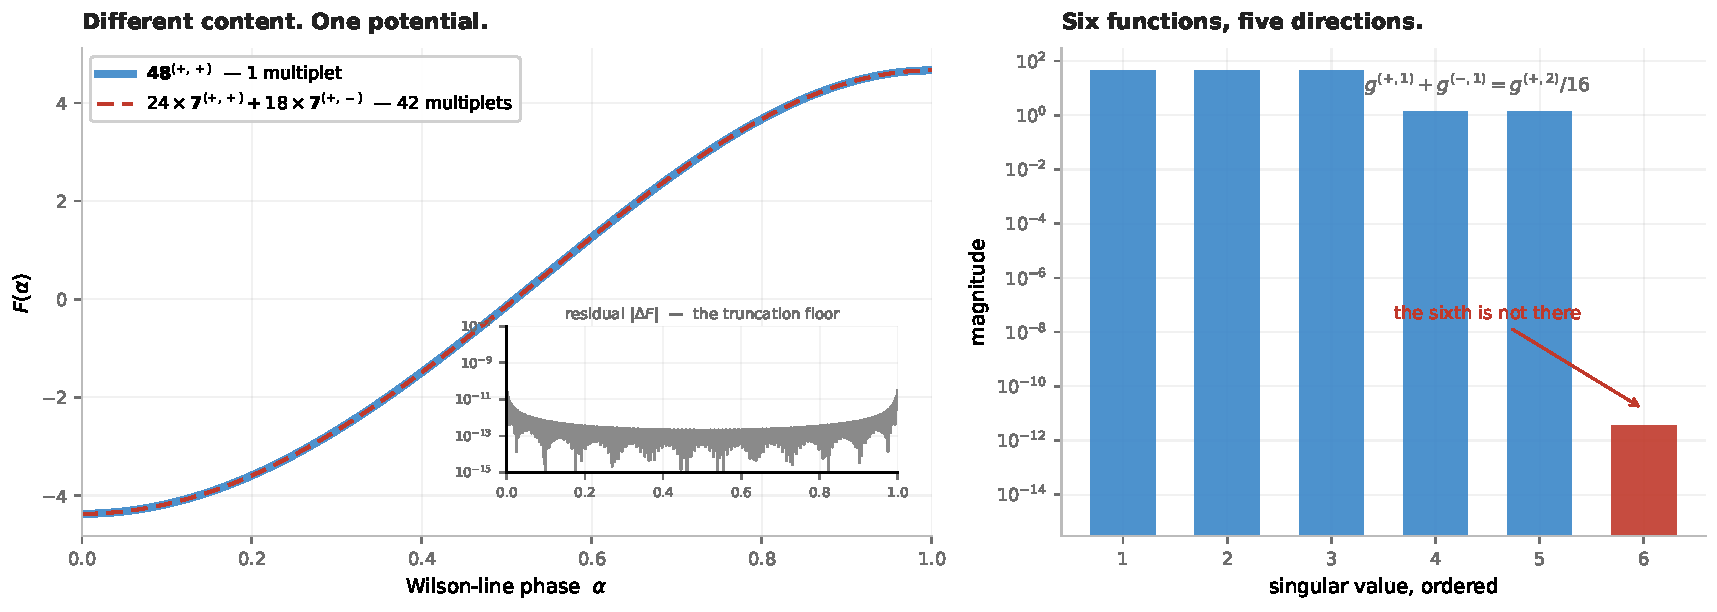
\includegraphics[width=\textwidth]{fig_kernel.pdf}
\caption{\textbf{Theorem~\ref{thm:complete}, in the two halves it is made of.} \emph{Left:} what it
asserts. A single $\rep{48}^{(+,+)}$ and $24\times\rep7^{(+,+)}+18\times\rep7^{(+,-)}$ --- one
multiplet against forty-two, different representations, different dimensions --- give
\emph{one curve}, on the exact polylogarithmic potential and across the whole fundamental domain.
The inset is the residual: over $1600$ points of $[0,1]$ its worst value is $2.9\times10^{-11}$,
which is not the identity failing but the floor
of this evaluation, the truncation of the winding sum at $600$ modes. The relation is exact over
$\mathbb{Q}$, proved in \texttt{dimension\_\allowbreak five.sage}. \emph{Right:} why it happens. The six
functions $\mathrm{Re}\,\mathrm{Li}_5(s\,e^{ic\pi\alpha})$ look like six directions and are five:
three singular values of order $45$, two of order $1.4$, and a sixth at
$3.5\times10^{-12}$ --- eleven orders below the smallest of the five. The missing one is the duplication
formula at $s=5$, which is \cite{CCD24}'s eq.~(2.11). A content is invisible to the potential
exactly when it is invisible to those five, which is the theorem. Drawn by
\texttt{make\_\allowbreak fig\_\allowbreak kernel.py}.}\label{fig:kernel}
\end{figure}

That is what makes the vertex decidable. At fixed $(A_4,8D)$ the condition $G\le G^\star$ reads
$U\ln2+V\ln3\ \ge\ \tfrac{25}{12}A_4-G^\star$: maximising a linear form over the contents with two
moments pinned. Every generator has $A_4\ge0$ and only $\rep7^{(+,+)}$ has $A_4=0$, whose
multiplicity is then forced by $8D$ --- so the feasible set is \emph{finite} and the maximum is a
computation, not a search. It comes out
\begin{center}\small
\begin{tabular}{crrr l}
\toprule
\rowcolor{hdrblue!10}$A_4$ on $8D=1$ & required & largest available & shortfall & \\
\midrule
\rowcolor{warmred!14}$215$ & $681.084$ & $681.017$ & $-0.067$ & no content, at any size\\
$212$ & $667.670$ & $669.927$ & $+2.257$ & attained\\
\bottomrule
\end{tabular}
\end{center}
\noindent so the relaxation's vertex is \emph{empty} and the one below it is not --- which is what
Figure~\ref{fig:lift} draws, rung by rung. The ceiling therefore has a witness, and the bound
sharpens:
\begin{keyeq}
\begin{equation}\label{eq:ceilinginteger}
  \boxed{\;\frac{1}{R_5}\;\le\;10.01\ \text{TeV}\;}
  \quad\text{optimum at } A_4=212,\ D=\tfrac18 .
\end{equation}
\end{keyeq}
\begin{figure}[t]\centering
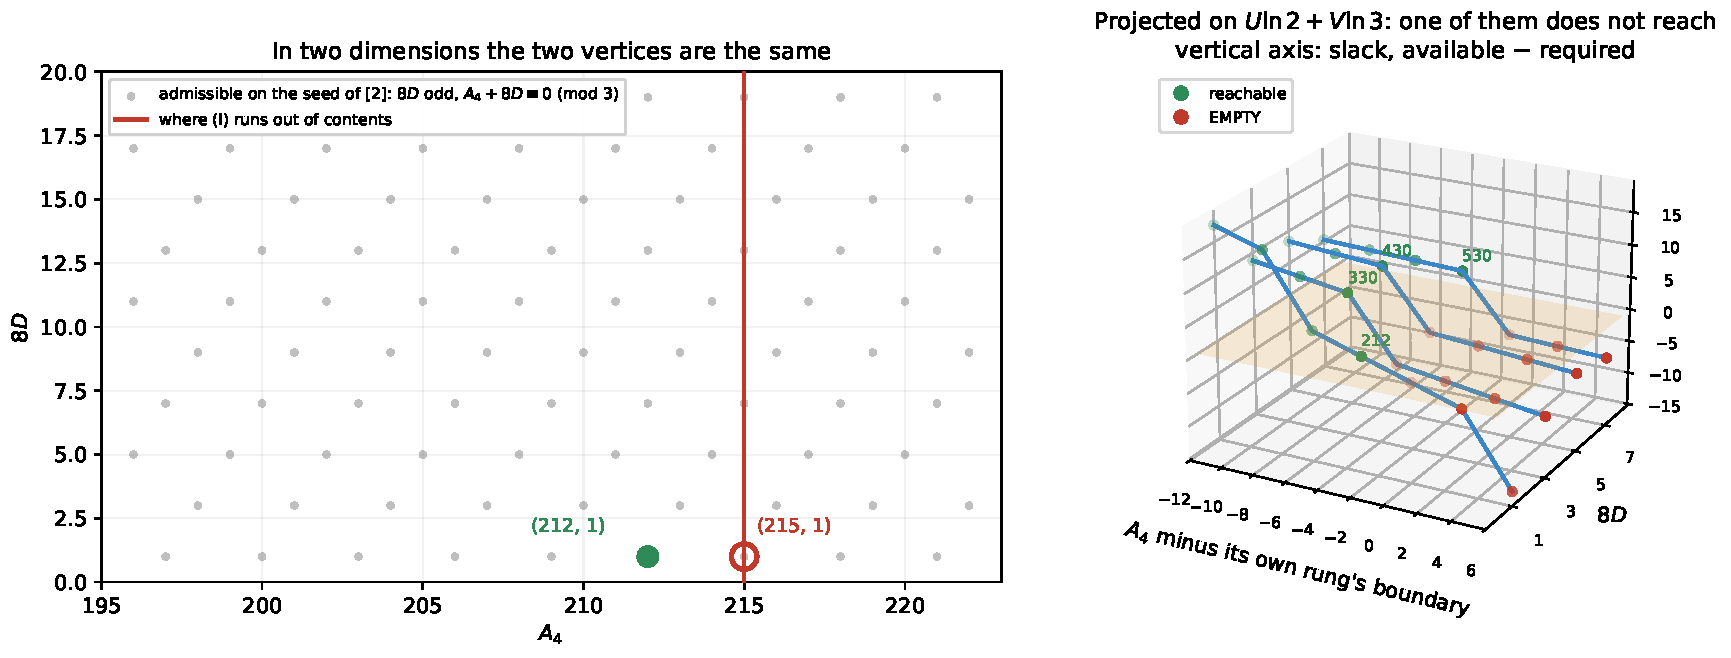
\includegraphics[width=\textwidth]{fig_lift.pdf}
\caption{\textbf{The axis the projection was hiding.} \emph{Left:} the plane the ceiling has been computed in. Both $(215,1)$ and $(212,1)$ are admissible lattice points --- $8D$ odd on the seed \cite{KM25} print, and $A_4+8D\equiv0\pmod 3$ --- and both sit at or under the boundary where identity~(I) runs out of contents. Nothing in this picture separates them. \emph{Right:} the same points with the third coordinate of \eqref{eq:UV}, plotted as the \emph{slack} between the logarithmic budget a content can supply and the budget $G\le G^\star$ demands; the raw budget runs past $680$ and the whole verdict is $0.067$ wide, so the slack is what can be drawn. Each rung is shown against distance to \emph{its own} boundary, which is what makes the four comparable. The amber plane is zero. Green is reachable, red is empty, and the green label is that rung's integer optimum. The slack falls monotonically, so each crossing is single and each optimum well defined --- and the pattern is the same on every rung: \textbf{the relaxation's boundary is empty and the integer optimum sits one or two steps of three below it}, at $212$, $330$, $430$, $530$ for $8D=1,3,5,7$. Drawn by \texttt{make\_\allowbreak fig\_\allowbreak lift.py}; the arithmetic is \texttt{semigroup.py}.}\label{fig:lift}
\end{figure}

\noindent The witness is
$17\times\rep7^{(+,+)}+2\times\rep7^{(+,-)}+57\times\rep{28}^{(+,-)}$, seventy-six multiplets ---
large, and nothing in the model caps the content, which was the point of \S\ref{sec:ceiling} to
begin with. Three things keep that honest. The $215$ verdict is checked at fifty digits and at both
ends of the Higgs window --- the smallest $G$ available there is $-233.100$ against a
$G^\star(127)=-233.168$, so it fails at the \emph{most permissive} end and therefore everywhere.
The witness is rebuilt through the ordinary \texttt{moments()} route, which knows nothing about $U$
and $V$, and reproduces $A_4=212$, $8D=1$, $G=-228.260$ inside the band. And the margin that
separates $215$ from $212$ is one part in $10^{4}$, an order below the closed form's own
$0.13$--$0.62\,\%$. Measured in \texttt{semigroup.py}.

\paragraph{And the ordering survives the truncation, which is not obvious and nearly failed.}
Everything so far lives on the surface \eqref{eq:amin}, which keeps three rungs; the discarded
remainder $R$ is bounded at the end of this section, in \eqref{eq:remainder}, and what is needed
here is only that it can be \emph{evaluated} on the handful of contents in question. Redoing the
elimination without discarding it gives the corrected pair
\begin{equation}\label{eq:corrected}
  x^2(6\mu+A_4)=12\zeta(3)D-\frac{18R'(x)}{x}+6R''(x)\,,\qquad
  \ln x=\frac{G-3\mu}{A_4}-\frac34+\frac{3\,[\,xR''(x)-R'(x)\,]}{A_4x^3}\,,
\end{equation}
so the demanded $G^\star$ moves by $\Delta G^\star=-3[xR''-R']/x^3$. Evaluated at the contents that
actually sit at these vertices, $\Delta G^\star\simeq-0.45$ at $(215,1)$ and $-0.33$ at $(212,1)$
--- \textbf{seven times the $0.067$ that separates them}. Comparing the correction with that gap is
therefore the wrong test, and it is worth saying why: $\Delta G^\star$ is \emph{common mode}, since
the contents at the two vertices differ by a few multiplets out of eighty. What it can do is eat
into each vertex's own slack, and that is the test:
\begin{center}\small
\begin{tabular}{crrrl}
\toprule
\rowcolor{hdrblue!10}vertex & slack, truncated & $\Delta G^\star$ & slack, corrected & \\
\midrule
\rowcolor{warmred!14}$(215,1)$ & $-0.067$ & $-0.452$ & $-0.519$ & still fails\\
$(212,1)$ & $+2.257$ & $-0.332$ & $+1.925$ & still holds\\
\bottomrule
\end{tabular}
\end{center}
\noindent \textbf{Both verdicts survive: $(215,1)$ fails by more once the truncation is carried, not
less, and $(212,1)$ keeps $1.93$ of slack.} What is not claimed is uniformity: $\Delta G^\star$ here
is evaluated on the finitely many named contents rather than bounded over all of them, which is
legitimate because they are finitely many and is not the same statement.

There is also a route needing no correction at all. At $(215,1)$ the smallest $G$ available over all
$26933$ contents is $-233.100$, while the Higgs window runs $[-238.553,-233.168]$; since $m_h$ is
monotone in $G$ at fixed moments --- $dG/d\mu=18\mu/(6\mu+A_4)>0$ --- every content there lies above
the window. That is an evaluation over a finite set. Measured in
\texttt{certify\_\allowbreak 212\_\allowbreak 215.py}.

\paragraph{And then the witness is put on the exact potential, and it fails a test the certificate
never applied.} A witness is a specific content, so it can be evaluated with no expansion at all:
minimise the polylogarithm numerically and look. The electroweak minimum is there and it is right
--- $\alpha=0.016129$ against the closed form's $0.016133$, agreement to $0.02\,\%$, better than on
any published row, with $m_h=126.25$~GeV inside the window. But the potential at the \emph{other}
symmetric point, $\alpha=1$, is $-204.99$ against $+111.44$ at that minimum. \textbf{The content
attaining the ceiling sits in a false vacuum.} The five published rows do not, which is the
control. Figure~\ref{fig:vacuum} is the two curves.

\begin{figure}[t]\centering
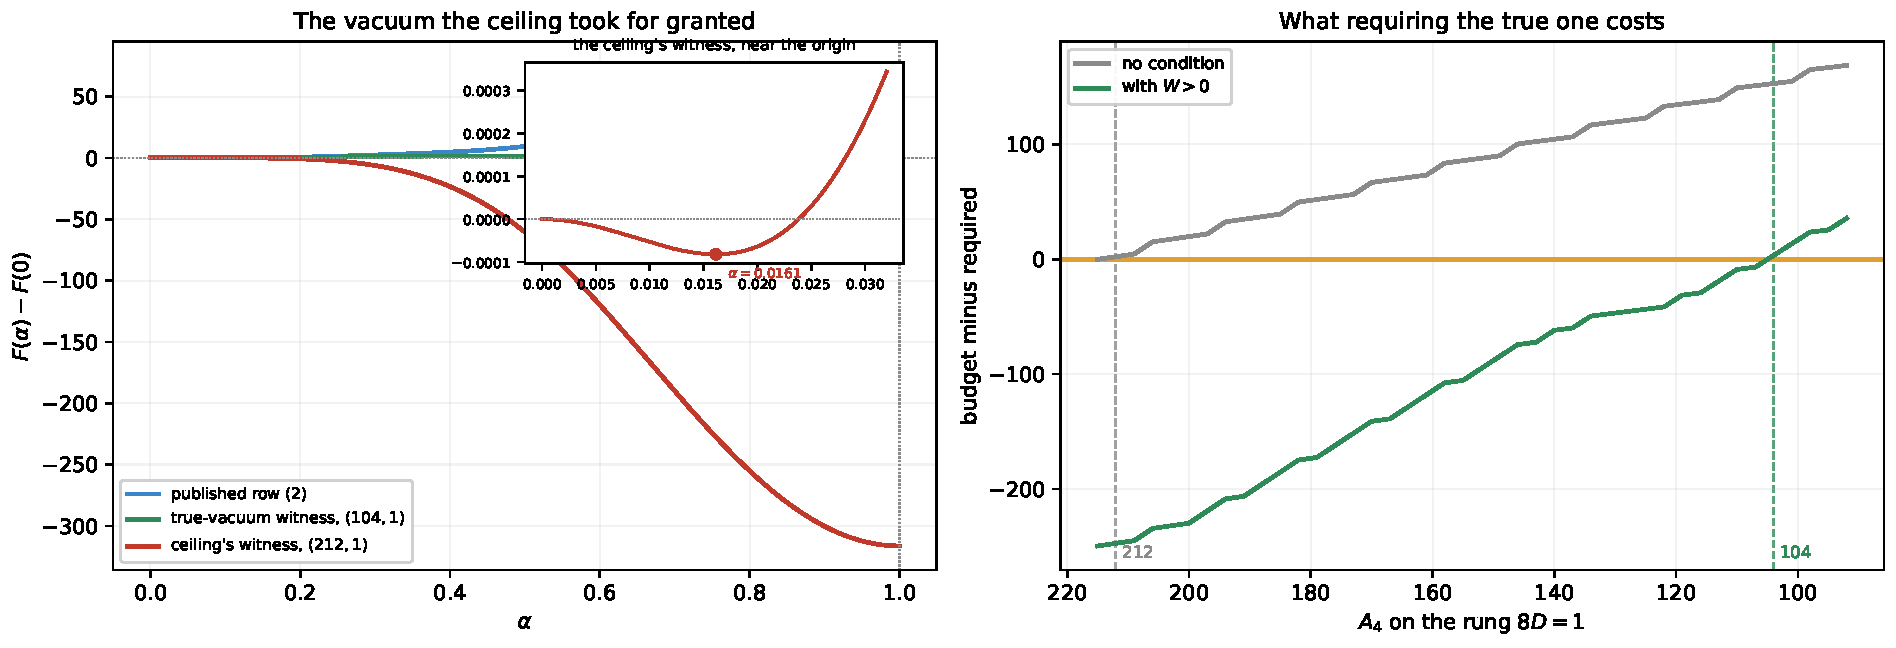
\includegraphics[width=\textwidth]{fig_vacuum.pdf}
\caption{\textbf{The vacuum the certificate took for granted.} \emph{Left:} the exact $F(\alpha)$ across the whole fundamental domain, each curve shifted so that $F(0)=0$. A published row rises to the right: its electroweak minimum is the deepest point there is. The content that attains $10.01$~TeV falls off a cliff instead --- at the other symmetric point $\alpha=1$ it is $316$ below the origin, so the minimum the ceiling was built on is a false one. The third curve is the content the constrained ceiling \eqref{eq:ceilingtrue} is attained by: it rises too, but only by $3.5$, which is why it hugs the axis at this scale --- passing the test is not the same as passing it comfortably. The inset is that same content near the origin, where its minimum is perfectly real and sits within $0.02\,\%$ of where \eqref{eq:amin} puts it: nothing is wrong with the closed form, only with the question it was asked. \emph{Right:} what excluding such contents costs. At each vertex of the rung $8D=1$, the largest logarithmic budget available minus the budget \eqref{eq:gstar} demands, with and without the stability condition $W>0$ of \eqref{eq:truevac}, which is \cite{CCD24}'s and not ours. The unconstrained curve crosses zero at $A_4=212$ and the constrained one not until $A_4=104$; the distance between those two crossings is $0.8$~TeV of ceiling. Drawn by \texttt{make\_\allowbreak fig\_\allowbreak vacuum.py}.}\label{fig:vacuum}
\end{figure}

\paragraph{The test it fails is not ours, and neither is the arithmetic of it.} Cacciapaglia
\emph{et al.}~\cite{CCD24} state the criterion and prove the identities it needs, in their
\S2.2. Their words: \emph{``it suffices to evaluate the potential at $a=0$ and $a=1/2$ and check
which configuration gives the smallest value''}; their eqs.~(2.12)--(2.13) give
$F_+(0)=\tfrac32\zeta(5)>0$ and $F_-(0)=F_+(1/2)=-\tfrac{15}{16}F_+(0)$, $F_-(1/2)=F_+(0)$; and
they draw the conclusion themselves --- components with parities $(\pm,\pm)$ stabilise the
starting orbifold and $(\pm,\mp)$ destabilise it. \textbf{The criterion, its arithmetic and its
sign rule are all theirs.} Summing their (2.13) over a bulk content in the bookkeeping of
\eqref{eq:F}, where their half-integer shift is our $\alpha\to\alpha+1$ and only odd charges
therefore move, gives
\begin{equation}\label{eq:truevac}
  F(1)-F(0)\;=\;\tfrac{31}{16}\,\zeta(5)\,W\,,\qquad W=\sum_{c\ \mathrm{odd}} m\,(-s)\,,
\end{equation}
with $\tfrac{31}{16}=1+\tfrac{15}{16}$, and $W>0$ sufficient for the electroweak point to be the
deeper one. That is their statement in our notation and nothing more; $W$ is their stabilising
count minus their destabilising one. What is new here is only what it is \emph{used for}: $W$ is
linear in the multiplicities, like $A_4$, $8D$ and $G$, so it can be carried inside the same
integer program --- and \cite{CCD24} do not compute a compactification scale, so they have no
program to carry it in. For this model the per-multiplet values are $\pm1,\pm3,\pm6,\pm9$ for
$\rep7,\rep{28},\rep{48},\rep{84}$ and $-\tfrac32$ for the gauge sector, the sign being the parity;
the five published rows have $W=\tfrac{63}{2},\tfrac{75}{2},\tfrac{75}{2},\tfrac{73}{2},\tfrac{69}{2}$
and the vertex at $(212,1)$ has $W=-\tfrac{315}{2}$. Checked
against the exact potential to machine precision on all six.

\paragraph{And $W$ cannot vanish --- for a sturdier reason than Theorem~\ref{thm:eighths}.} Matter
contributes integers to $W$. The gauge sector does not: its odd-charge part is
$2-\tfrac72=-\tfrac32$. Hence $2W$ is an odd integer for every bulk content, and with
\eqref{eq:truevac},
\begin{keyeq}
\begin{equation}\label{eq:nevermarginal}
  \frac{32}{31}\,\frac{F(1)-F(0)}{\zeta(5)}\ \text{is an odd integer, so}\quad
  |F(1)-F(0)|\;\ge\;\tfrac{31}{32}\,\zeta(5)\,.
\end{equation}
\end{keyeq}
\noindent \textbf{In this model the two symmetric points are never degenerate} --- and the scope of
that sentence is not decoration, because in other models of the same architecture they are: see
below.

\noindent \textbf{And this one holds on both branches, which the odd eighths do not.} It is
tempting to file it with Theorem~\ref{thm:eighths} as the same half-integer read twice, and an
earlier version of this paper did. The candidate seed of \S\ref{sec:open} separates them. It moves
the two charge-one weights by the same $+\tfrac12$, and $2W$ depends on the \emph{difference}
$-u_{(+,1)}+u_{(-,1)}$, in which that shift cancels exactly: $2W$ stays $-3$. The gauge
contribution to $8D$ does not cancel and moves by $9$, losing its parity. \emph{So $2W$ odd is
seed-robust and $8D$ odd is not} --- and we would not have known which was which with one seed to
look at. Verified over all $3003$ contents of at most six multiplets:
none has $W=0$ and none has $2W$ even.

That matters more than a curiosity, because it closes a question \cite{CCD24} raise themselves. In
their models the degeneracy \emph{does} occur, twice and exactly: their eq.~(3.14) is a function of
$2a$ alone, and their eq.~(3.44) is invariant under the simultaneous shift
$(a,b)\to(a+\tfrac12,b+\tfrac12)$, so in both cases the two symmetric points are degenerate and
they read it correctly --- the two are then \emph{``two equivalent descriptions of the same
orbifold''}. Were that the case here, a potential deeper at $\alpha=1$ would be a relabelling and
not a false vacuum at all. But equivalent descriptions must give equal potentials, and
\eqref{eq:nevermarginal} says the two values are never equal --- so for this model the deeper
configuration is a genuinely different orbifold, and the reading above stands.

\noindent \textbf{And the whole difference between the two situations is one number.} The
architecture is shared: \cite{HHK03} likewise reduce their vacuum energy to integer functionals and
likewise find that a signed parity count decides between two symmetric configurations. But their
gauge sector contributes the \emph{even integer} $+2$ to their $a$ and nothing at all to their $b$,
so both can vanish --- they open their classification with ``the case with $a=0$'' and list
$n_F^{(+)}=n_F^{(-)}\Rightarrow$ ``completely degenerate'' as an ordinary case (their eqs.~(4.14),
(4.15)). Here the gauge sector contributes a \emph{half}-integer to $W$ --- $2-\tfrac72=-\tfrac32$ on the
seed \cite{KM25} print and $\tfrac32-3=-\tfrac32$ on the candidate one, the same number both times
because $W$ reads the difference --- and a half-integer cannot be cancelled by integers. \textbf{The degenerate case they enumerate is, in this model, arithmetically
unreachable.} Measured in \texttt{W\_\allowbreak is\_\allowbreak half\_\allowbreak odd.py} and
\texttt{hhk\_\allowbreak gauge\_\allowbreak offset.py}. The criterion remains theirs; what is added
is that here it can never tie.

\paragraph{The ceiling, with the vacuum required to be the true one.} Imposing $W>0$ alongside
$G\le G^\star$ and walking the rung down, no vertex survives until $A_4=104$:
\begin{keyeq}
\begin{equation}\label{eq:ceilingtrue}
  \boxed{\;\frac{1}{R_5}\;\le\;9.22\ \text{TeV}\;}
  \quad\text{optimum at } A_4=104,\ D=\tfrac18,\ \text{true vacuum required.}
\end{equation}
\end{keyeq}
\noindent The witness is
$16\times\rep7^{(+,+)}+\rep{28}^{(+,-)}+\rep{48}^{(+,+)}+4\times\rep{48}^{(+,-)}+\rep{84}^{(+,+)}$,
twenty-three multiplets, $W=\tfrac52$; and on the \emph{exact} polylogarithmic potential its global
minimiser is $\alpha=0.017560$, with $m_h=126.00$~GeV and $1/R_5=9157$~GeV. \textbf{That last
number is a statement about the potential and not about any expansion.}

\paragraph{And there is a second number, because $127$ is not a mass the Higgs has.} Every ceiling
here is evaluated at the top of \cite{KM25}'s window $[125,127]$, which is the right end for an
upper bound: $\mu\propto m_h^2$, so by (II) the ceiling rises with $m_h$, measured and not assumed.
But the measurement is $m_h=125.20\pm0.11$~GeV, and $127$ sits $16.4$ standard deviations above it.
Evaluated instead at the mass the Higgs actually has, the vertex drops a whole lattice step and so
does the answer:
\begin{keyeq}
\begin{equation}\label{eq:ceilingmeasured}
  \boxed{\;\frac{1}{R_5}\;\le\;9.09\ \text{TeV}\;}
  \quad\text{at } A_4=101,\ \text{measured Higgs mass.}
\end{equation}
\end{keyeq}
against $9.22$~TeV at $A_4=104$ over the window --- $1.4\,\%$, and a step of three in $A_4$. The
one-sigma band does \emph{not} move the vertex, $125.09$ and $125.31$ both giving $101$, so
\eqref{eq:ceilingmeasured} is stable against the measurement and unstable only against the width of
a window nobody is obliged to use. The same substitution takes the unconstrained ceiling from
$10.01$ to $9.87$~TeV. Both statements are true and they are not the same statement: $9.22$~TeV
bounds any content whose Higgs mass lies \emph{anywhere} in $[125,127]$, and $9.09$~TeV bounds any
content whose Higgs mass is the measured one. \textbf{A reader wanting a number about the world
should take the second.} The window is kept for the headline because it is \cite{KM25}'s and
because a bound quoted over a stated window is the safer object. Measured in
\texttt{higgs\_\allowbreak window.py}.

\paragraph{And it explains a gap this paper had left unexplained.} The table above tops out at
$9156$~GeV while the certificate says $10034$, and that difference was called the gap between a
relaxation and its lattice. It is not. The enumeration used the \emph{global} minimiser, so it had
been screening false vacua all along without saying so; the certificate screened nothing. Both of
its champions have $W>0$ --- $\tfrac{31}{2}$ at $N=8$ and $\tfrac52$ at $N=14$ --- and evaluated exactly they give
$9139$ and $9157$~GeV, which are the two numbers already in the table. \textbf{The constrained
optimum \emph{is} the enumeration's champion}, and a gap that looked like insufficient search was a
physical condition nobody had written down. Measured in \texttt{socratic\_\allowbreak witness.py}
and \texttt{vacuum\_\allowbreak constraint.py}.

\paragraph{And the last approximation left \emph{inside} \eqref{eq:F} is the truncation, and it
is bounded rather than estimated.} Everything above except the two exact evaluations is computed on the surface
\eqref{eq:amin}, which keeps three rungs of the ladder. Write $F=F_0+R$, with $R$ the part from
$k\ge3$. Two classical facts make $R$ boundable and neither is ours: $\zeta(5-2k)=-B_{2k-4}/(2k-4)$
with $|B_{2n}|\le(\pi^2/3)(2n)!/(2\pi)^{2n}$ \cite{Apostol}, and the expansion itself \cite{Lewin}.
Bounding the bracket of \eqref{eq:ladderab} by the fourth moment, $A_4+B_4$, and summing the
geometric series gives, for $u=c_{\max}\alpha<1$,
\begin{equation}\label{eq:remainder}
  |R(\alpha)|\;\le\;\frac{\pi^{6}S_4\,c_{\max}^{2}\,\alpha^{6}}{2160\,(1-u^{2})}\,,\qquad
  |R'(\alpha)|\;\le\;\frac{\pi^{6}S_4\,c_{\max}^{2}\,\alpha^{5}}{360\,(1-u^{2})}\,.
\end{equation}
Put to a falsification attempt on $32$ contents at four values of $\alpha$ each --- the attempt
being to find one violation, and the outcome that there are none, tightest slack
$1.4\times$. Two controls, and both can fail: the bound \emph{refuses} to return anything at
$u\ge1$, where the true remainder does blow up; and it is a bound and not an estimate --- the sharp
estimate is $(A_6+3B_6)x^6/8640$, which is not rigorous, and mixing the two would be the easiest
mistake here. An earlier version of \eqref{eq:remainder} was off by a factor, and the falsification
is what caught it.

\paragraph{Using it naively is worthless, and that is the instructive part.} Replacing each rung's
$1/R_5$ by its rigorous upper value and re-maximising does \emph{not} give a rigorous ceiling of
$10$~TeV: it gives $52.429$~TeV, and the maximum migrates from $8D=1$ to $8D=139$. The margin grows
with $A_4$ while the truncated value falls, so the rungs that lose on the truncated surface win on
the bounded one. \textbf{A bound on the remainder is not automatically a bound on the optimum}, and
the distinction is not formal: taking it seriously moves the answer by a factor of five.

\paragraph{What repairs it is not a better inequality but not needing one.} The charges run over
$c\in\{1,2,3\}$ and there are two parities, so the potential is spanned by six functions
\emph{however much matter there is} --- five, in fact, and the reduction is \emph{not ours}. The
polylogarithm duplication formula $\mathrm{Li}_s(z)+\mathrm{Li}_s(-z)=2^{1-s}\mathrm{Li}_s(z^2)$
\cite{Wood} at $s=5$ gives $g^{(+,1)}+g^{(-,1)}=g^{(+,2)}/16$, and \cite{CCD24} already writes
exactly this in exactly this setting --- their eq.~(2.11), $F_-(a)=-F_+(a)+\tfrac1{16}F_+(2a)$,
repeated in \cite{Cac25} eq.~(3.3). There is no second relation of that kind here because $c=4$ and
$c=6$ are not charges of this model, so the six span five. What is used below is only that the
number is finite; and the statement is about \eqref{eq:F}, the $n^{-5}$ part of \cite{KM25}'s
potential, not about their full winding weight, which mixes powers and does not close on five.
Hence
$R(\alpha)=R_{\text{gauge}}(\alpha)+\sum_j n_j R_j(\alpha)$ exactly --- the same shape as $A_4$,
$8D$, $G$ and $W$. The margin is therefore itself a linear functional and goes inside the very dual
that produces the certificate, with the $G\le G^\star$ constraint released so that the answer stays
a bound and the dual stays two-variable. That move is ordinary linear programming \cite{Schrijver}
and is claimed as nothing more. Over $70$ rungs:
\begin{keyeq}
\begin{equation}\label{eq:rigorousceiling}
  \boxed{\;\frac{1}{R_5}\;\le\;10.037\ \text{TeV}\;}
  \quad\text{untruncated, over the first $70$ odd rungs.}
\end{equation}
\end{keyeq}
\noindent The maximum stays on $8D=1$ across those seventy; the margin over the truncated
certificate is $2.5$~GeV, or $0.025\,\%$; and against the $52.429$~TeV of the uniform route it is
a factor of four thousand. So the truncation is worth two and a half GeV, not two and a half TeV,
and \S\ref{sec:ceiling} is not an artefact of keeping three rungs.

\noindent\textbf{And seventy rungs is where the statement stops, which an earlier version of
this paragraph did not say.} It read ``arbitrary content'', and that is false: the remainder
\emph{bound} loosens with the rung even as the truncated ceiling falls. Its relative bite
$\delta/\hat x$ runs from $2.5\times10^{-4}$ at $8D=1$ to $9.1\times10^{-2}$ at $8D=129$ and
$9.0\times10^{-1}$ at $8D=1201$ --- a factor of three thousand six hundred, and at that last rung
the bound eats nine tenths of the phase it is meant to certify. The scan there returns
$27.8$~TeV --- not because the ceiling rises there, but because the bound stops saying anything.
\textbf{The truncated ceiling is untouched by this}: \eqref{eq:slope} and the sign of
$\partial\Phi/\partial k$ prove $M(k)\le6268$~GeV for every $k\ge3$, all rungs, no scan. What is
restricted to seventy is \eqref{eq:rigorousceiling} alone, and closing it needs a remainder
bound uniform in the rung, which \S\ref{sec:open} now asks for.

\paragraph{And what in that is still numerical care rather than proof.} Three places, named because
a reader will find them otherwise. $R'_j$ is a central difference rather than an analytic
derivative, which the term-by-term expansion would fix immediately. The step $\delta$ uses the
curvature \emph{at} $\hat x$ rather than its minimum over $[\hat x-\delta,\hat x]$; at
$\delta/\alpha=2.5\times10^{-4}$ nothing moves, but the clean statement needs the minimum. And the
winding sums are truncated at $4000$, where the tail is $4\times10^{-15}$ against $|R'|\sim10^{-6}$.
None of the three is a gap in the argument; all three are places where interval arithmetic would
replace care with proof. Finally, \eqref{eq:rigorousceiling} is the \emph{unconstrained} ceiling:
the true-vacuum condition has not been carried through the same machinery, and since it only
removes contents, what may be said about \eqref{eq:ceilingtrue} untruncated is this, and it is
deliberately three statements rather than an interval. \emph{The exact-potential witness gives
$9157$~GeV} --- which needs no bound at all, being an evaluation. \emph{Over the first seventy odd
rungs the untruncated potential is bounded above by $10.037$~TeV.} \emph{A global untruncated upper
bound, over arbitrary multiplicities and hence over all rungs, remains open}, and \S\ref{sec:open}
names the missing piece: a remainder bound uniform in the rung. Writing those three as a single
interval $[9157\,\text{GeV},10.037\,\text{TeV}]$ would assert the third, and the third is precisely
what is not proved. Measured in \texttt{remainder\_\allowbreak theorem.py},
\texttt{rigorous\_\allowbreak ceiling.py} and \texttt{rigorous\_\allowbreak ceiling2.py}.

\paragraph{And $W>0$ is \emph{necessary} exactly where the bound is decided, which makes
\eqref{eq:ceilingtrue} a statement about every content and not about a screened family.} Proving
necessity in general is not required: a content only matters if it \emph{beats} $9.22$~TeV, and
such a content has $\alpha<2m_W/9220=0.01744$, that is $x<0.0548$. Two facts then collide. The gap
at the other symmetric point is quantised and cannot be small --- by \eqref{eq:nevermarginal},
$W<0$ forces $F(1)\le F(0)-\tfrac{31}{32}\zeta(5)=F(0)-1.0045$. And the electroweak well is
microscopic, which is visible once its depth is written out: eliminating $G$ with stationarity and
then $A_4$ with (II) collapses it to two terms,
\begin{equation}\label{eq:depth}
  F(x_\star)-F(0)\;=\;-\,\frac{\zeta(3)D\,x_\star^{2}}{8}\;-\;\frac{\mu\,x_\star^{4}}{16}\,,
\end{equation}
which reproduces the exact well to between $0.00$ and $0.16\,\%$ on the five published rows and on
the witness --- better than the closed form's own accuracy, because the error cancels between the
two eliminations. On the rung $8D=1$, and at $x<0.0548$, that depth is at most $1.03\times10^{-4}$.

The argument is then three lines. Only the rung $8D=1$ can exceed $9.22$~TeV, since the certificate
already bounds $8D=3$ at $6.27$~TeV and every rung above it lower. So $D=\tfrac18$ and the well is
shallower than the quantised gap by a factor of $9755$. If $W<0$, then
$F(1)\le F(0)-1.0045<F(0)-1.03\times10^{-4}\le F(x_\star)$, so the electroweak point is not the
global minimum and the content was not a candidate after all. $W=0$ is arithmetically impossible.
Hence $W>0$, and the integer program over $W>0$ has already been run.
\textbf{$1/R_5\le9.22$~TeV therefore holds for any bulk content whose electroweak point is its true
vacuum} --- the screen was never a restriction where the bound is decided. The reach of the
argument is $8D<17815$, far beyond any rung that could compete. Measured in
\texttt{necessity\_\allowbreak of\_\allowbreak W.py}. What it does \emph{not} remove is the other
caveat: step one uses the per-rung certificate, whose globality rests on the monotonicity of
$t^\star(k)/k$ --- which \eqref{eq:dphidk} now proves rather than measures.

\paragraph{And it is \emph{sufficient} there too, because the screen can be replaced by the thing
it stands for.} Necessity leaves the other half open: $W>0$ compares the electroweak point with the
\emph{other symmetric point} only, and a third minimum somewhere in $(0,1)$ would be seen by
neither. That half is settled by not screening at all. If the electroweak point is the global
minimum then for every $y$
\begin{equation}\label{eq:semiinf}
  F(y)-F(0)\;\ge\;F(\alpha_{\text{EW}})-F(0)\;=\;-\,\bigl|\text{well}\bigr|\;\ge\;-\Theta ,
\end{equation}
where $\Theta$ denotes the bound on the well depth supplied by \eqref{eq:depth} --- a separate
letter from the $\Delta$ of \eqref{eq:moments}, which is a moment of the content and not a
depth. The left-hand side is \emph{linear} in the multiplicities --- the same shape as $A_4$, $8D$,
$G$ and $W$ --- while $\Theta$ is a constant of the rung. So ``the
electroweak point is the global minimum'' is a semi-infinite integer program: solve with the cuts
in hand, minimise the incumbent over $y$, add the cut where it is violated, repeat. It must be
anchored at the origin and not at $x_\star$. The exact condition \emph{is} $F(y)\ge F(x_\star)$
for all $y$ --- that is what a global minimum means, and it is not stronger than the truth but
the truth itself. What cannot be carried into a linear program is its right-hand side, which
depends on the content through $x_\star$ and its depth. Replacing it by the uniform bound
$F(0)-\Theta$ keeps the program linear and keeps the relaxation \emph{weaker} than the truth,
which is the direction an upper bound needs: a maximum over too small a feasible set is not an
upper bound at all.

Three things make it terminate. The cut at $y=1$ \emph{is} the screen, since \eqref{eq:semiinf}
there reads $\tfrac{31}{16}\zeta(5)W\ge-\Theta$ and $2W$ odd then forces $W\ge\tfrac12$ as soon as
$\Theta<1.0045$ --- at the deciding vertex $\Theta=1.02\times10^{-3}$, which is deliberately ten
times the depth bound above and not a restatement of it, three orders of room even so, so the
screen is a corollary of the programme rather than an input to it. The function space is finite, as
above. And the eight multiplets are only \emph{five} directions in it: the kernel of
content~$\mapsto$~potential has dimension three, with three relations of non-negative coefficients.
Boldface is the representation and the upright digit before $\times$ is its multiplicity, so the
third line has one $\rep7^{(+,+)}$ and not seven of anything:
\begin{equation}\label{eq:fivegen}
\begin{aligned}
  \rep{28}^{(+,+)}&=20\times\rep7^{(+,+)}+17\times\rep7^{(+,-)}, &
  \rep{48}^{(+,+)}&=24\times\rep7^{(+,+)}+18\times\rep7^{(+,-)},\\
  \rep{48}^{(+,-)}&=1\times\rep7^{(+,+)}+4\times\rep7^{(+,-)}+1\times\rep{28}^{(+,-)}, & &
\end{aligned}
\end{equation}
so the fibre over $(A_4,8D)$ is small enough to enumerate exhaustively. \textbf{That such
degeneracies exist is \cite{CCD24}'s}: their \S3.3 exhibits two models with different matter and
the same gauge-scalar potential and calls it accidental, and their eqs.~(3.25)--(3.27) are their
own eq.~(2.11) producing one. What is added here is that the accident is a subspace and can be
listed: the kernel has dimension three and \eqref{eq:fivegen} spans it. The third relation is also
Part~VI's, found there for the opposite purpose --- the two sides have different $\sum C_2$, so the
degeneracy dies at two loops; the other two need thirty-seven and forty-two multiplets and that
search was capped at six. Verified in exact rational arithmetic in \texttt{dimension\_\allowbreak
five.sage} on a retyped matrix.

\paragraph{And the coefficients being non-negative is worth a corollary.} A relation with a
negative coefficient would rewrite a content as a formal \emph{difference} of contents, which is
not a content. All seven coefficients in \eqref{eq:fivegen} are non-negative integers, so the
rewriting never leaves the physical cone: every bulk content has a one-loop-equivalent
representative built from five types only,
\begin{equation}\label{eq:canonfive}
\begin{aligned}
  N_{\rep7^{(+,+)}}&=n_{\rep7^{(+,+)}}+20\,n_{\rep{28}^{(+,+)}}+24\,n_{\rep{48}^{(+,+)}}+n_{\rep{48}^{(+,-)}},\\
  N_{\rep7^{(+,-)}}&=n_{\rep7^{(+,-)}}+17\,n_{\rep{28}^{(+,+)}}+18\,n_{\rep{48}^{(+,+)}}+4\,n_{\rep{48}^{(+,-)}},\\
  N_{\rep{28}^{(+,-)}}&=n_{\rep{28}^{(+,-)}}+n_{\rep{48}^{(+,-)}},
\end{aligned}
\end{equation}
the two $\rep{84}$'s carrying through unchanged. The five are independent and minimal --- deleting
any one drops the rank to four --- so this is a change of basis and not a projection.

\noindent\textbf{The consequence, at its real strength.} It is tempting to record this as a
normality theorem: the semigroup equals its cone intersected with its lattice, no holes. That is
true, and it is not a theorem. Writing $B$ for the five generators, \eqref{eq:canonfive} makes
$S=B\NN^5$, $L=B\ZZ^5$ and $C=B\RR_{\ge0}^5$, so $x\in C$ \emph{is} $B^{-1}x\ge0$ and $x\in L$
\emph{is} $B^{-1}x$ integral; ``no holes'' restates the definitions. What should be said instead
is the shorter and stronger thing: \textbf{the semigroup of one-loop potentials is free on five
generators, $S\cong\NN^5$.} Free, not merely normal --- there is nowhere to put a hole. All the
content is in \eqref{eq:canonfive} and none of it in the deduction. Inverting $B$ then turns the
five complete invariants into five canonical multiplicities, so the congruences of
\S\ref{sec:ceiling} are the condition that $B^{-1}$ return integers and the cone inequalities are
$N\ge0$.

\noindent\textbf{And this does not settle the question \S\ref{sec:open} asks.} That question is
whether the \emph{lifted} semigroup is normal in the four coordinates $(A_4,8D,2U,V)$, and
projection does not preserve normality: a point can lie in the projected cone and the projected
lattice while every preimage of it falls outside the cone. What the corollary changes is what a
hole would \emph{mean}. No potential is missing. A four-coordinate hole would record a
$(A_4,8D,2U,V)$ whose required $2W$ no content supplies --- a gap in the coordinate that was
dropped, not in the space of potentials. Checked, with the controls that can fail separated from
the ones that cannot, in \texttt{canonical\_\allowbreak five.py}.

\textbf{On the rung $8D=1$ the programme stops at $A_4=104$ having generated exactly one cut, the
one at $y=1$} --- and it is generated at $A_4=212$ by the content of Figure~\ref{fig:vacuum}
itself, which the programme identifies as a false vacuum without being told. So where the bound is
decided, $W>0$ is not merely necessary: it is the
\emph{whole} of the true-vacuum condition, and \eqref{eq:ceilingtrue} is a bound over every bulk
content whose electroweak point is its vacuum. \textbf{The worry is not empty, though --- it is
real and it does not reach.} On $8D=3$ the oracle demands a second cut, forced by
$6\times\rep7^{(+,+)}+\rep7^{(+,-)}+5\times\rep{28}^{(+,-)}+\rep{48}^{(+,-)}+2\times\rep{84}^{(+,+)}$,
which has $W=\tfrac12$ and so \emph{passes} the screen, yet sits $4.82$ below the origin there ---
far deeper than its own well. The oracle returns that cut as a number, $y=0.6809$, and it need not
be one. Since $\mathrm{Li}_5(z)+\mathrm{Li}_5(-z)=2^{-4}\mathrm{Li}_5(z^{2})$ puts every term of the
potential in the span of $P_q(y)=\mathrm{Re}\,\mathrm{Li}_5(e^{iq\pi y})$ with $q\in\{1,2,3,4,6\}$
--- Theorem~\ref{thm:complete} read off the phases rather than off the moments --- and since every
$P_q(2/3)$ is an exact rational multiple of $\zeta(5)$, the depth at the rational holonomy $y=2/3$
is a closed-form linear functional of the content, in the same sense that $F(1)-F(0)=\tfrac{31}{16}
\zeta(5)W$ is: writing $F=\sum_qC_qP_q$,
\[
  F(\tfrac23)-F(0)\;=\;-\tfrac{121}{81}\,\zeta(5)\,\bigl[\,C_1+C_2+C_4\,\bigr],
\]
which on this content is $-\tfrac{1331}{288}\zeta(5)=-4.7922$, some $579$ times the allowance at
the vertex that forced it, $\Theta(147,3)=8.28\times10^{-3}$ --- and $\Theta$ is per vertex, eight
times the $1.02\times10^{-3}$ of the deciding one, so it is the rung's own allowance that is used
here. So the second cut can be taken exactly, and the disqualification never rests
on a numerical minimum. A third minimum invisible to both symmetric points exists and binds; it
simply binds on a rung the ceiling does not live on. \emph{What does not follow} is that the cuts
are rational in general: over all $6560$ contents of multiplicity at most two the global minimiser
is strictly interior in $2956$ cases, those sit a mere $1.05$ times closer to $\{1/3,1/2,2/3\}$ than
a uniform draw on the same range, and \emph{not one} of the three skeleton bins is so much as a
local maximum of where they land. The one excess that is there --- $32.5\,\%$ of them in
$[0.20,0.30)$ against a uniform $12.7\,\%$ --- sits against the electroweak end and not at any
rational. The charge alphabet supplies a skeleton; it does not generate the cuts. Both measured, in
\texttt{rational\_\allowbreak holonomies.py} and \texttt{holonomy\_\allowbreak skeleton.py}.
Finally the winning witness is
taken off the grid altogether: with the winding tails bounded by
$\sum_{n>N}n^{k-5}\le N^{k-4}/(4-k)$ and $|F^{(k+1)}|\le\sum|m|(c\pi)^{k+1}\zeta(4-k)$ closing the
gaps between grid points, $F''<0$ from the origin with $F'(0)=0$ exactly, then $F'<0$, then a
convex window containing a sign change of $F'$, then a certified margin of $0.42$ on the rest of
$[0,1]$: \textbf{its electroweak point is the global minimum of $F$ on $[0,1]$}, not merely the
better of two symmetric points. Measured in \texttt{semi\_\allowbreak infinite.py}.

So there are two ceilings and they answer different questions. $10.01$~TeV bounds any content whose
electroweak point is stationary, which is what an integer program over the moments can see;
$9.22$~TeV bounds any content whose electroweak point is also the \emph{vacuum}, which is what the
model has to mean. The second is the physical one. The first is kept because the argument that
produces it is what makes the second computable, and because the distance between them is the
price of a question the certificate cannot ask.

\paragraph{Controls.} Every champion of that curve was re-minimised numerically on the original
potential rather than trusted to the closed form: the worst error is $+0.62\,\%$, on the row of
largest $\alpha$, and every champion's $m_h$ is still inside $125$--$127$~GeV at the numerical
$\alpha$. The certified ceiling dominates all $1097$ window contents found up to $N=14$. And the
control that must fail does: ignoring Theorem~\ref{thm:mod6} places the optimum on the phantom point
$(216,1)$ and inflates the ceiling by $7$~GeV.

\paragraph{And Part~VI's escape moves it.} Part~VI \cite{PartVI} obstructs the one-generation
version of this model and classifies the minimal escapes; the surviving one is a family-dependent
charge that must be hosted by an $\rep{84}^{(+,+)}$ donated to the brane, which removes it from the
Higgs potential. The lattice of \S\ref{sec:arith} prices that donation without a new computation:
the host carries $8D=+10$, so paying for the escape costs exactly $10/8$ of $D$.
Electroweak breaking needs $D>0$, and $8D$ is odd by Theorem~\ref{thm:eighths} on the seed
\cite{KM25} print, so
\begin{equation}\label{eq:escapebound}
  \text{a content can afford the escape}\quad\Longleftrightarrow\quad 8D\;\ge\;11 ,
\end{equation}
an integer condition with no slack in it. The per-$D$ ceiling is monotone
decreasing, so \eqref{eq:escapebound} does not merely forbid contents --- it forbids the rungs the
ceiling lives on. Running the same exact rational dual over every odd rung from $11$ upwards:
\begin{keyeq}
\begin{equation}\label{eq:escapeceiling}
  \boxed{\;\frac{1}{R_5}\;\le\;3.97\ \text{TeV}\;}
  \quad\text{for any content that can afford the escape.}
\end{equation}
\end{keyeq}
\noindent Against $10.03$~TeV without it, both on the seed \cite{KM25} print --- a factor $2.53$.

\noindent\textbf{The quantum does the work twice.} The unconstrained ceiling sits \emph{on} $8D=1$, and the
escape's bill is exactly what makes that rung unaffordable: the content that generates the largest
hierarchy is the one that cannot pay. The enumeration respects the bound --- of the $1097$ window
contents at $N\le14$, $857$ can still afford it, and the best of those reaches $3017$~GeV. Scope,
and it has to be said whole: this bounds the content \emph{before} the donation, the row that pays.
It does not bound the world after, whose bulk needs only $8D\ge1$.

\paragraph{And it answers a question Part~VI could only state.} Part~VI asks, in its own list of
what it does not claim, whether a row that pays for the escape still lands in the Higgs window
afterwards --- and says the modified potential is not recomputed there, because doing so needs a
closed form for $\amin$ it does not have. This paper has one, so the question is now arithmetic.
Donating one $\rep{84}^{(+,+)}$ from each published row and re-minimising through \eqref{eq:two}:
\begin{center}\small
\rowcolors{2}{white}{softgrey}
\begin{tabular}{ccc}
\toprule
\rowcolor{hdrblue!10}row & $8D$ after donating & $m_h$ after\\
\midrule
\rowcolor{amber!12}(1) & $5$  & $145.6$~GeV\\
\rowcolor{amber!14}(2) & $19$ & $114.7$~GeV\\
\rowcolor{warmred!13}(3) & $-1$ & no interior minimum\\
\rowcolor{amber!12}(4) & $1$  & $169.0$~GeV\\
\rowcolor{amber!12}(5) & $5$  & $145.6$~GeV\\
\bottomrule
\end{tabular}
\end{center}
\noindent \textbf{None of the five lands in $125$--$127$~GeV once the host is donated}, and case~(2)
--- the row Part~VI selects as the only one that can \emph{pay} --- comes out lowest of the four
that still break. Paying for the escape and keeping the Higgs mass are therefore two different
demands, and the five published rows satisfy them one at a time. Every $m_h$ here is a
\emph{measured} number and carries the anchor residual of \S\ref{sec:setting}; what does not is the
$8D$ column, which is the arithmetic of \S\ref{sec:arith}.

\paragraph{Scope of the ceiling.} No further physical condition is imposed on the lattice --- not
six-dimensional anomaly freedom, not perturbativity. That is the safe direction: any such criterion
can only \emph{remove} contents, so the bound stands, while the champion content would move.
Figure~\ref{fig:surface} is that ceiling drawn as an explicit surface over the two quantised moments.

\begin{figure}[t]\centering
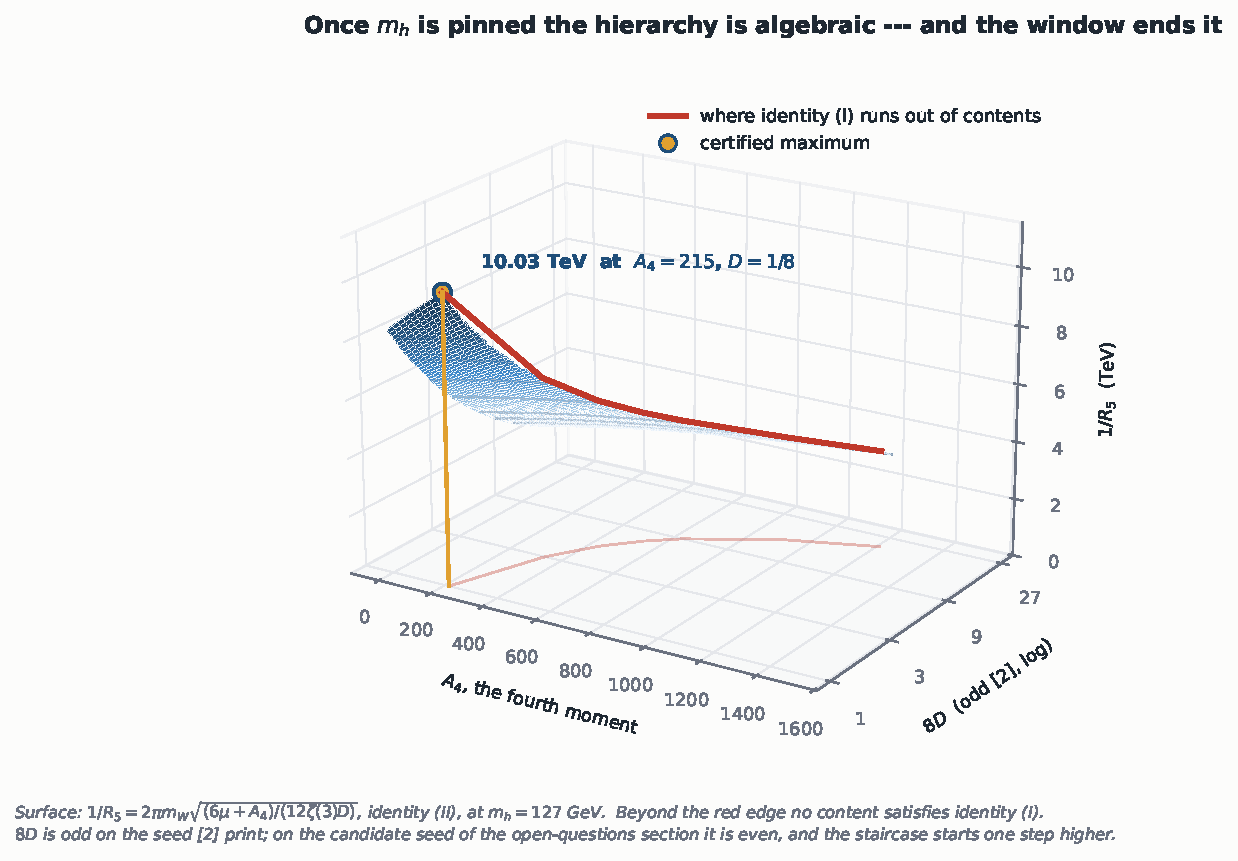
\includegraphics[width=\textwidth]{fig_surface.pdf}
\caption{\textbf{The ceiling's geometry.} Once $m_h$ is pinned, identity (II) makes $1/R_5$ an explicit surface over the two quantised moments, with no minimisation left in it. The red curve is where identity (I) runs out of contents: beyond it the lattice cannot supply a $G$ small enough. The maximum of the surface over the feasible region is the certified ceiling, and it sits on the smallest positive rung the arithmetic admits.}\label{fig:surface}
\end{figure}

\bridge{A bound is only worth stating if something can be done with it --- and the same two integers
that produced it also say where, inside the bound, the answer is allowed to sit.}

% ===================================================================
\section{What this predicts}\label{sec:pred}

\paragraph{Anchor-free, and arithmetic --- but not equally.} The congruence
$8D-2A_4\equiv0\pmod6$ is a property of the matter lattice alone: no normalisation, no loop order,
no scheme, and no gauge sector either. The \emph{parity} of the total $8D$ is a different animal:
it is fixed by the gauge base point, and \S\ref{sec:open} is about which base point that is.
Both are still tests a reader can run on someone else's table in a minute; only the first is a test
of the content rather than of the seed. Their own five rows pass both.

\paragraph{A correlation, not two numbers.} $\amin$ and $m_h$ are functions of the same two moments,
so they are not independent data. Pinning $m_h$ to the measured value \emph{fixes} $1/R_5$ from the
content through (II), with no minimisation --- which is what makes the ceiling computable at all.

\paragraph{And the Kaluza-Klein scale is not a continuum: it sits on an arithmetic comb.} Cross (II)
with Theorem~\ref{thm:mod6} and something falls out that neither says alone. Writing $k=8D$ and
$M_{\mathrm{KK}}=1/R_5=2m_W/\amin$, (II) reads
\begin{equation}\label{eq:comb}
  M_{\mathrm{KK}}^{2}\;=\;\frac{8\pi^2m_W^2}{3\zeta(3)}\;\frac{6\mu+A_4}{k}\,,
\end{equation}
and Theorem~\ref{thm:mod6} fixes $A_4$ modulo three once $k$ is fixed, so at fixed $k$ and fixed
$m_h$ the admissible $A_4$ advance in steps of three and
\begin{equation}\label{eq:comb2}
  M_{n+1}^{2}-M_{n}^{2}\;=\;\frac{8\pi^2m_W^2}{\zeta(3)\,k}\,,
\end{equation}
independent of the content and of the Higgs mass. \textbf{The exactly-spaced quantity is $M^2$, not
$M$}, and a spacing in mass is $\Delta M=\Delta M^2/2M$, so it is meaningless without saying at which
$M$ --- and each rung has its own ceiling, so quoting them all at one mass quotes most of them where
they cannot reach. At $k=1$ the step is $0.42$~TeV$^2$, which at that rung's own ceiling of
$10$~TeV is $21$~GeV in mass; at $k=11$ the step is $0.039$~TeV$^2$ and the ceiling is $3.97$~TeV,
so $4.9$~GeV. The statement is
\emph{necessary and not sufficient} --- every realisable content lands on a tooth, not every tooth
holds a content --- and the \emph{position} of the comb carries the anchor residual and the choice of
$g_4$ while its \emph{spacing} does not, being arithmetic. Read as a test it is unusual: given
$m_h$, $m_W$, $g_4$ and a candidate Kaluza-Klein resonance, one may ask whether any admissible pair
$(k,A_4)$ reproduces it. \textbf{Which pairs are admissible belongs to the seed and not to the
lattice}: on the seed \cite{KM25} print the test reads $k$ odd, $A_4\in\ZZ$ and
$A_4+k\equiv0\pmod3$, while on the candidate seed $k$ is even and $A_4\in\ZZ+\tfrac12$. What
survives either is Theorem~\ref{thm:mod6} written so that every entry is an integer on both
seeds --- $A_4$ is half-integral on the candidate one, $2A_4$ is not --- namely
$k-2A_4\equiv3\pmod6$ with $(2A_4,k)\in\ZZ^2$. The
spacing is the matter lattice's and the offset is the affine coset's, which is the same split
\S\ref{sec:open} turns on. Verified against the certificate row of
\S\ref{sec:ceiling} in \texttt{crossed\_\allowbreak equations.py}.

\paragraph{And the ceiling has collider teeth.} A bound
on $1/R_5$ is a bound on a compactification scale and not on a single resonance mass.
\cite{KM25}'s eqs.~(18)--(19) expand the mixed-parity components in
$\cos\bigl((n+\tfrac12)x_5/R_5\bigr)$, so those towers are half-integer-moded and their lightest
state sits at $1/(2R_5)$, while the unbroken gauge bosons keep integer levels $n/R_5$. Which of
them a given search bounds, with what coupling to the fixed-point quarks and what width, is fixed
by the same parities and is derived in \S\ref{sec:collider}; the short answer is that the
half-integer tower is a colour singlet and the only coloured state below the Planck scale is the
gluon tower at $n/R_5$. Carrying the anchor residual of
\S\ref{sec:setting} through:

\begin{center}\small
\rowcolors{2}{white}{softgrey}
\begin{tabular}{lrr}
\toprule
\rowcolor{hdrblue!10} & our normalisation & $\times$ the largest measured ratio\\
\midrule
content of their own size ($\le6$ multiplets) & $2.18$~TeV & $4.53$~TeV\\
ceiling over \emph{all} contents & $10.03$~TeV & $20.82$~TeV$^{\dagger}$\\
\rowcolor{amber!14}ceiling once the vacuum must be the true one & $9.22$~TeV & $19.14$~TeV$^{\dagger}$\\
ceiling for contents that can afford the escape & $3.97$~TeV & $8.24$~TeV$^{\dagger}$\\
\bottomrule
\end{tabular}
\end{center}

\noindent At the mass the Higgs actually has, rather than at the top of \cite{KM25}'s window, the
highlighted row reads $9.09$~TeV --- \eqref{eq:ceilingmeasured}, and the benchmark to quote at the
physical mass, carrying the same two caveats as every theory-side scale here. The right-hand column is not carried across for it, being an
extrapolation already.

\noindent The highlighted row is the physical one: the row above it allows contents whose
electroweak point is stationary without being the minimum, and \S\ref{sec:ceiling} shows the
content that saturates it is exactly of that kind. The $10.03$ is kept because it is the bound the
certificate proves for arbitrary content, and because the difference between the two rows --- eight
hundred GeV --- is what one physical condition is worth.

\noindent$^{\dagger}$\emph{Extrapolations, not bounds.} The right-hand column multiplies by $2.076$,
the largest ratio measured on the five published rows. That is legitimate for the first row, whose
contents are of their own size and sit inside the anchored range. It is not for the other two: by
\S\ref{sec:setting} the ratio is a trend rather than scatter, and the two ceilings sit outside the
range that measures it --- the first in $D$ ($1/8$ against $[1.125,3.625]$), the second in $A_4$
($727$ against $[189,271]$). The trend rises towards the first of those corners, so $20.8$ is if
anything an under-estimate of where the rescaled ceiling would sit; but it is an extrapolation of
five points, and it is written here as one.

\noindent Against published exclusions --- a Kaluza-Klein gluon below roughly $4$~TeV, a sequential
$Z'$ below roughly $5$~TeV --- the small-content corner of the class, which is the corner their
Table~1 populates, is already disfavoured, and that is a consequence of the closed form rather than
of any new measurement. The ceiling then caps the whole class. And the escape bound of
\eqref{eq:escapeceiling} bites harder: $3.97$~TeV sits in a region dijet data are highly sensitive
to, and the rescaling that would lift it to $8.24$~TeV is the extrapolation flagged above, not a
bound, so the sensitivity is not evaded by appealing to it. \textbf{And the recast is now done,
which is what puts a number on the other side at all.} It could not be taken from the generic Kaluza-Klein gluon limits
quoted above --- those are for a \emph{narrow} resonance, while \S\ref{sec:collider} derives this
object's own width, $\Gamma(G^{(n)}\!\to q\bar q)/M_n\simeq0.16$, and the $s$-channel rate would
additionally need $\mathrm{BR}(G_1\to jj)$, which the model does not fix. The spacelike form
factor \eqref{eq:resum} needs neither, and carried through \cite{CMSangular}'s published
covariance it gives a nominal recast sensitivity of $1/R_5>10.86$~TeV, rising to $13.75$~TeV on
the mass range \cite{CMSangular} themselves use for contact interactions. \textbf{So the branch
that can also pay for Part~VI's escape from proton decay, at $3.97$~TeV, sits a factor of three
below where this recast loses sensitivity.} \S\ref{sec:collider} says how, why that is not yet
the word \emph{excluded}, and what would make it one.

\begin{keyeq}
The prediction is bounded \emph{above}, which is the useful direction: \textbf{the model cannot
retreat to higher scales by adding matter.} Adding matter raises $A_4$, and a larger $A_4$ raises
$1/R_5$ only until the Higgs window closes it off --- which is precisely what the integer program
measures. An analysis with demonstrated sensitivity to \emph{this} tower across the algebraically
allowed mass range could therefore test the three-rung class --- a weaker claim than saying a
machine of some beam energy settles it, and the right one: \S\ref{sec:collider} says which
resonance, why reach and beam energy are not the same number, and what still stands between a
sensitivity and an exclusion.
\end{keyeq}

\paragraph{A prediction inside someone else's framework.} Equation~\eqref{eq:valuebound} says that
the orbifold-stability criterion of \cite{CCD24}, applied to this model, is never marginal. That is
a statement in their language, about their question, checkable against their own code.

\bridge{A ceiling on a compactification scale is not a ceiling on anything a detector records.
Which state would a search actually be bounding, with what coupling and what width --- and is any
of that ours to choose?}

% ===================================================================
\section{Which state a search bounds}\label{sec:collider}

A bound on $1/R_5$ is a bound on a compactification scale, not on the mass of any one particle. A
collider does not measure compactification scales; it measures resonances, each with a production
rate and a width. Getting from one to the other looks like it needs a phenomenological study, and
it does not: it is fixed by the three parity matrices of \cite{KM25} and the mode expansions that
follow from them, all of which are already published. This section reads them.

\paragraph{The parity that separates colour.} Of the three $\ZZ_2$ matrices, the one acting in
$x_6$ is
\begin{equation}\label{eq:P6}
  P_6=\mathrm{diag}(+,+,+,-,-,-,-),
\end{equation}
\cite{KM25}'s (11), which splits the seven-dimensional index into the colour triplet and
everything else. A gauge component along $E_{ij}$ carries the \emph{product} $P_6^{(i)}P_6^{(j)}$,
so \eqref{eq:P6} has an immediate consequence that is arithmetic rather than dynamical:
\begin{equation}\label{eq:colourparity}
  P_6(i,j)=-1
  \quad\Longleftrightarrow\quad
  \text{exactly one of } i,j \text{ is a colour index,}
\end{equation}
that is, precisely when the generator changes colour. There are $24$ such components, and there is
no colour-changing component with $P_6=+1$.

\begin{theorem}[colour lives on the small circle]\label{thm:colourparity}
Every colour-changing gauge boson of \cite{KM25} has $P_6=-1$. By its (21)--(24) each such
component expands in $\sin(m x_6/R_6)$ with $m\ge1$. Hence its lightest level is at least $1/R_6$,
and its wavefunction \emph{vanishes} at $x_6=0$.
\end{theorem}
\begin{proof}
\eqref{eq:colourparity} is the statement that $P_6^{(i)}P_6^{(j)}=-1$ iff one index lies in the
colour block, which is immediate from \eqref{eq:P6}. The four $P_6$-odd expansions of \cite{KM25},
its (21)--(24), all carry $\sin(m x_6/R_6)$ and all start at $m=1$; the sine vanishes at the
origin and the level is bounded below by the $m=1$ term.
\end{proof}

\noindent This matters because \cite{KM25} p.~3 fixes $R_5\gg R_6$ and calls $1/R_6$ ``an
arbitrary parameter, which is the Planck scale for instance''. Theorem~\ref{thm:colourparity} then
says the coloured exotics have no tree-level coupling to the brane quarks at all, and that in the
$R_5\gg R_6$ hierarchy the model intends they lie far beyond collider reach. Neither statement is
that they are unobservable in principle: $1/R_6$ is called arbitrary rather than fixed, and a
coloured $X_m$ is still a bulk gauge field, so the vertex $g^{(0)}X_mX_m$ carries
$\int\!\mathrm{d}x_6\,\sin^2(mx_6/R_6)\neq0$ and QCD pair production survives the vanishing of the
single-$X$ vertex. What the theorem removes is the direct channel, which is the one that matters
for proton decay.

\paragraph{So the brane quarks see exactly two towers.} \cite{KM25} p.~22 introduces ``quarks
$q_L,u_R,d_R$ as the 4D fermions on the brane at the origin in a compactified space $(0,0)$''. A
4D field there couples only to components whose mode function is non-zero at that point --- that
is, to components whose $x_5$ \emph{and} $x_6$ factors are both cosines. Of the eight parity
classes only two qualify, and both are colour-diagonal:

\begin{center}\small
\rowcolors{2}{white}{softgrey}
\begin{tabular}{llllll}
\toprule
\rowcolor{hdrblue!10} parity & eq. & $x_5$ mode & $x_6$ mode & at $(0,0)$ & lightest level\\
\midrule
$(+,+,+)$ & (17) & $\cos(nx_5/R_5)$ & $\cos(mx_6/R_6)$ & \textbf{non-zero} & $0$, then $1/R_5$\\
$(+,+,-)$ & (18) & $\cos((n{+}\tfrac12)x_5/R_5)$ & $\cos(mx_6/R_6)$ & \textbf{non-zero} & $1/(2R_5)$\\
$(+,-,+)$ & (19) & $\sin((n{+}\tfrac12)x_5/R_5)$ & $\cos(mx_6/R_6)$ & zero & $1/(2R_5)$\\
$(+,-,-)$ & (20) & $\sin(nx_5/R_5)$ & $\cos(mx_6/R_6)$ & zero & $1/R_5$\\
$(-,\cdot,\cdot)$ & (21)--(24) & --- & $\sin(mx_6/R_6)$ & zero & $\ge 1/R_6$\\
\bottomrule
\end{tabular}
\end{center}

\noindent The $(+,+,-)$ class is exactly the two positions $(6,7)$ and $(7,6)$ --- a colour
singlet. So the half-integer tower, whose lightest state sits at $1/(2R_5)$ and which
\S\ref{sec:pred} correctly flagged as the lowest level in the model, is \emph{not} something a
dijet search can see; and it is not a clean prediction either, since $\langle W\rangle$ of
\cite{KM25}'s (77) acts in the $(5,7)$ block and shifts it with $\alpha$. The one coloured object
below the Planck scale is the gluon tower.

\paragraph{And that answers a question \cite{KM25} left open.} Their conclusions read: ``Since the
mass of $X$, $Y$ gauge bosons is small in our model, this causes rapid proton decay \emph{if they
can couple to quarks and leptons}'', and they leave the question to future work. By
Theorem~\ref{thm:colourparity} they cannot: the $X$ and $Y$ bosons are precisely the
colour-changing components, and their wavefunction is zero at the fixed point where the same paper
puts the quarks. The gauge-exchange channel is shut by the parity assignment itself.

\noindent\textbf{The scope of that is narrow and worth stating.} It is a tree-level statement about
gauge exchange, for the quarks localised as in \cite{KM25} p.~22. It says nothing about the brane
Dirac masses that same paper introduces on p.~16 to lift its unwanted zero modes, and it is
\emph{not} the escape of Part~VI \cite{PartVI}, which is a family-dependent charge hosted by a
donated $\rep{84}^{(+,+)}$ --- a different mechanism, addressing a different operator. In
particular \eqref{eq:escapeceiling} is untouched by it.

\paragraph{The coloron's mass and quark coupling are fixed --- and neither is new.} Three facts fix
it, and all three are results of other people applied here rather than found here. The mass: \cite{KM25} p.~16
states that the $\su3_C$ generators ``are commutable with $\langle W\rangle$ irrespective of the
VEV $\alpha_{\min}$'', so the colour tower takes no Wilson-line shift and sits at $n/R_5$ exactly.
The coupling: their (17) carries $\sqrt2$ in front of every $(n,0)$ mode where the zero mode
carries $1$, and $\cos(0)=1$, so at the brane the ratio is $\sqrt2$ --- and it is
flavour-universal, because $q_L$, $u_R$ and $d_R$ sit at the same point and see the same mode
function. The width then follows from the standard colour-octet result
$\Gamma(C\to q\bar q)=n_f\,\alpha_s\cot^2\theta\,M/6$ with $\cot^2\theta=2$ and $n_f=6$:

\begin{keyeq}
\begin{equation}\label{eq:coloron}
  M_n=\frac{n}{R_5},
  \qquad
  \frac{g_{G^{(n)}q\bar q}}{g_{gq\bar q}}=\sqrt2,
  \qquad
  \frac{\Gamma(G^{(n)}\!\to q\bar q)}{M_n}=2\alpha_s(M_n)\simeq0.16 .
\end{equation}
\end{keyeq}

\noindent \textbf{Whose result each of those is.} The $\sqrt2$ of a Kaluza-Klein gauge boson
on a brane-localised fermion, and the width $\Gamma_n=2\alpha_s m_n$ that goes with it, are
\cite{DMN01}, whose Lagrangian --- gauge fields in the bulk, quarks held at $y=0$ by a delta
function --- is structurally the setup of \cite{KM25}. The colour-octet Lagrangian and the width
formula are \cite{Simmons97}; the production cross section at next-to-leading order is
\cite{Chivukula13}; and a Kaluza-Klein gluon confronted with a dijet distribution in a
gauge-Higgs model is \cite{KS16}, who also note that $\sqrt2 g_s$ is the \emph{largest} coupling
available and carry a free parameter below it. What is specific here is only that
\cite{KM25} puts its quarks exactly at the fixed point, so the bound is saturated rather than
assumed --- and that \eqref{eq:ceiling} caps the scale from above, which is what makes any of
these numbers testable at all. Carried across the rows of \S\ref{sec:pred}:

\begin{center}\small
\rowcolors{2}{white}{softgrey}
\begin{tabular}{lrrrr}
\toprule
\rowcolor{hdrblue!10} & $1/R_5$ & $\alpha_s$ & $\Gamma/M$ & $\Gamma$\\
\midrule
\rowcolor{amber!14}ceiling at the measured $m_h$ & $9.09$~TeV & $0.0735$ & $0.147$ & $1337$~GeV\\
ceiling once the vacuum must be the true one & $9.22$~TeV & $0.0734$ & $0.147$ & $1354$~GeV\\
ceiling over \emph{all} contents & $10.03$~TeV & $0.0729$ & $0.146$ & $1463$~GeV\\
contents that can afford the escape & $3.97$~TeV & $0.0789$ & $0.158$ & $626$~GeV\\
\bottomrule
\end{tabular}
\end{center}

\paragraph{Which changes what may be quoted against it.} A width of one sixth of the mass is not a
narrow resonance, so the narrow benchmark of a dijet search does not bound this object: CMS's
$6.6$~TeV for a narrow axigluon or coloron at $137\,\mathrm{fb}^{-1}$ \cite{CMSdijet} is a limit on
a different particle. What does apply is the model-independent limit on $\sigma\,B\,A$ that the
same analysis publishes as a function of mass \emph{and} width, read at $\Gamma/M\simeq0.16$. The
previous version of this section compared \eqref{eq:escapeceiling} to a generic Kaluza-Klein gluon
exclusion; \eqref{eq:coloron} is what makes that comparison a statement about this model rather
than about a benchmark, and it is the reason the comparison is worth making at all.

\paragraph{A correction to how the reach was stated.} An earlier version of this paper wrote that a
machine reaching $10$--$20$~TeV settles the class. That conflates the energy of a collider with its
reach in resonance mass, and the two are not the same: producing a $9$~TeV resonance at
$\sqrt s=13$~TeV requires partons at values of $x$ where the parton densities are negligible. The
correct statement is about mass reach in the relevant channel, and it makes the escape branch far
more interesting than the ceiling --- $3.97$~TeV sits where Run~2 has real sensitivity, while
$9.09$~TeV does not.

\paragraph{The tower also acts below the first resonance.} Since every $(n,0)$ mode has the same
$\sqrt2$ at $x_5=0$, integrating out the whole tower gives a colour-octet four-quark operator with
a coefficient that is a pure number:
\begin{equation}\label{eq:tower}
  \sum_{n\ge1}\frac{g_n^2}{2M_n^2}
  \;=\;g_s^2R_5^2\sum_{n\ge1}\frac{1}{n^2}
  \;=\;\frac{\pi^2}{6}\,g_s^2R_5^2 ,
  \qquad\text{i.e.}\qquad
  \Lambda_8=\frac{\sqrt3}{\pi\sqrt{\alpha_s}}\,\frac{1}{R_5},
\end{equation}
which is $7.79$~TeV on the escape branch and $18.48$~TeV at the measured-$m_h$ ceiling.
\textbf{Two things must be said about those two numbers before anyone compares them with a
published limit.} First, \eqref{eq:tower} is the leading term of an expansion in
$\hat s/M_1^2$, and the dijet data that would test it sit at $M_{jj}\sim2$--$8$~TeV --- which is
\emph{on} the tower when $1/R_5=3.97$~TeV, not below it. There the contact operator is the wrong
object and the exact tree-level statement is the replacement of the gluon propagator by
$1/q^2+\sum_n 2/(q^2-M_n^2+iM_n\Gamma_n)$ of \cite{DMN01}, which is what
\texttt{kk\_\allowbreak dijet\_\allowbreak lo.py} evaluates. \textbf{Second, and it replaces a
correction an earlier version of this section carried}: that propagator does not need to be
truncated in the spacelike channels, and it must not carry a width there. For $t<0$ every mode
sits below its two-parton threshold, so the self-energy has no absorptive part and the propagator
is real; and with all $c_n$ equal --- which is Theorem~\ref{thm:colourparity} together with
\cite{KM25}'s localisation of the quarks at the fixed point, and is what makes the sum
$\sum_n(n^2+a^2)^{-1}$ rather than an arbitrary one --- Euler's expansion does it in closed form.
Writing $a=R_5\sqrt{-t}$,
\begin{keyeq}
\begin{equation}\label{eq:resum}
  \frac{1}{q^2}+\sum_{n\ge1}\frac{2}{q^2-n^2/R_5^2}\;=\;\frac{\mathcal F(q^2)}{q^2}\,,\qquad
  \mathcal F(q^2)=
  \begin{cases}
    \pi a\coth(\pi a)\,, & a=R_5\sqrt{-q^2}\,,\quad q^2<0\,,\\[2pt]
    \pi b\cot(\pi b)\,,  & b=R_5\sqrt{q^2}\,,\quad q^2>0\,.
  \end{cases}
\end{equation}
\end{keyeq}
\noindent so the whole coloured tower is one \emph{form factor} on the gluon propagator. The
resummation is standard --- it is how a brane-to-brane propagator is written, and the identity goes
back to Euler; what is specific here is that the universal $\sqrt2$ makes it available at all. Three
things follow at once. Its expansion $\pi a\coth\pi a=1+\pi^2a^2/3-\pi^4a^4/45+\cdots$ returns
$-\pi^2R_5^2/3$, which is \eqref{eq:tower}: the contact operator is the first term of
\eqref{eq:resum} and not an independent statement. On a subprocess with only $t$-channel exchange
the parton-level ratio is exactly $\mathcal F^2$, and with $|t|=M_{jj}^2/(1+\chi)$ that is a closed
form in the two variables the measurement is binned in. And \emph{it does not depend on
$\mathrm{BR}(G_n\to jj)$}, because nothing is produced and decayed --- which is the one thing the
model does not supply, below. \textbf{The $2.55\,\%$ width correction to $\Lambda_8$ that stood
here is therefore withdrawn}: it came from inserting a fixed $iM_n\Gamma_n$ where there is no
absorptive part to insert, and the giveaway is that the shift does not switch off as $t\to0$ but
tends to $1/(1+(2\alpha_s)^2)$, which no self-energy below threshold may do. The zero-width
$\pi^2/6$ is the right coefficient, not an approximation to a better one. Measured in
\texttt{kk\_\allowbreak resummation.py}.

\noindent\textbf{And the second line of \eqref{eq:resum} collapses this section into one
statement.} Nothing in the sum required $q^2<0$; that was only where the width could be dropped.
The same expansion continues to the timelike side by $\coth(ix)=-i\cot x$, so a single analytic
function covers the whole tree-level tower. Then the three things this section has been saying
separately are three regions of it. The contact operator \eqref{eq:tower} is its expansion about
$b=0$. The angular distortion of Figure~\ref{fig:tower} is its spacelike branch. And \emph{the
resonances are the poles of the cotangent}, at $b=1,2,3,\dots$, that is $\sqrt{q^2}=n/R_5$ ---
they are not put in by hand and no truncated sum is needed to find them; they are where the closed
form diverges, and they are precisely and only where a width must replace the pole. So the
amplitudes read $\mathcal M_{qq\to qq}=\mathcal M_{\mathrm{QCD}}[\mathcal F(t),\mathcal F(u)]$ and
$\mathcal M_{q\bar q\to q\bar q}=\mathcal M_{\mathrm{QCD}}[\mathcal F(s),\mathcal F(t)]$, and the
width enters exactly one of the four arguments. Both branches checked against the sum in
\texttt{kk\_\allowbreak resummation.py}.

\noindent\textbf{And the second circle is genuinely UV-sensitive, so what has to be quoted is its
coefficient and not its absence.} An earlier version of this paragraph said the logarithmic
divergence one would fear from a codimension-two brane ``never switches on''. It does: a
two-dimensional tower is logarithmically sensitive to the cut-off and no hierarchy removes that.
What the hierarchy suppresses is the coefficient, and the same Euler identity gives it. Summing
$n$ first at fixed $m$, $\sum_{n\in\ZZ}(n^2/R_5^2+m^2/R_6^2)^{-1}=\pi R_5(R_6/m)\coth(\pi
mR_5/R_6)\to\pi R_5R_6/m$ for $R_5\gg R_6$, so
\begin{equation}\label{eq:codim2}
  \frac{\Delta C_{m\ge1}}{C_{m=0}}\;=\;\frac{6}{\pi}\,\frac{R_6}{R_5}\,\ln(\Lambda R_6)\,,
\end{equation}
logarithmic in the cut-off with one power of $R_6/R_5$ in front --- $1.3\,\%$ at $R_5/R_6=10^3$
and a cut-off a decade above $1/R_6$, and far less at the $1/R_6$ \cite{KM25} p.~3 contemplates.
Verified against the direct double sum in \texttt{kk\_\allowbreak resummation.py}. This is a collective prediction of
the tower and does not require resolving any resonance; it cannot, however, be compared directly
with published compositeness scales, whose operator has a different colour and chiral structure.

\paragraph{And one number the model does not supply.} \cite{KM25} p.~16 lifts its unwanted zero
modes by introducing ``4D fermion conjugate to the representations and charges of the massless
fermions and their Dirac mass terms on the fixed points'', and does not fix those masses. If any
coloured exotic sits below $M/2$ then $G^{(1)}\to\Psi\bar\Psi$ opens, the width grows and
$\mathrm{BR}(G^{(1)}\to jj)$ falls by an amount nothing here determines. So
\begin{equation}\label{eq:brhole}
  \mathrm{BR}(G^{(1)}\to jj)=1 \quad\text{if every coloured exotic lies above } M/2,
\end{equation}
and less otherwise. That single unknown is what stands between the arithmetic ceiling and a
model-specific exclusion, and a limit quoted without it would be model-independent in appearance
only. It is stated here rather than absorbed.

\paragraph{And that unknown points at a different measurement than one would expect.} A resonance
search looks for a bump, and a bump is only the first rung of \eqref{eq:coloron} --- so its rate
carries precisely the branching ratio that \eqref{eq:brhole} declines to fix. But the quarks of
\cite{KM25} sit at a point, so they see \emph{every} rung with the same $\sqrt2$, and what the
whole tower does is not to add a peak: it replaces the gluon propagator by
$1/q^2+\sum_n2/(q^2-M_n^2+iM_n\Gamma_n)$ --- in \emph{every} channel, $t$ and $u$ as well as
$s$, which is how \cite{DMN01} write it. Well below the first rung the change is a constant,
$-\tfrac{\pi^2}{3}R_5^2$, so the \emph{relative} change grows with $|q^2|$; and at fixed dijet
mass $|t|=M_{jj}^2/(1+\chi)$ is largest at small $\chi$. The effect is therefore central, and
the observable is the angular distribution rather than the mass spectrum.

\noindent There is a measurement built for exactly that. \cite{CMSangular} reports
$\chi_{\mathrm{dijet}}$ at $138\,\mathrm{fb}^{-1}$ \emph{corrected for detector effects} and
compared with QCD at next-to-next-to-leading order, quoting a total theoretical uncertainty of
$3.5\%$ in its $3.0$--$3.6$~TeV mass bin. Being unfolded, it can be confronted with a calculation
directly. Evaluating \eqref{eq:resum} in the lowest $\chi$ bin of that same mass range gives a
ratio to QCD of $1.36$ at the measured-$m_h$ ceiling and $3.16$ on the escape branch, against the
$1.3$ and $3.4$ the all-channel calculation of \texttt{kk\_\allowbreak dijet\_\allowbreak lo.py}
returns at the same point --- the two agree to a per cent and a half where they should;
Figure~\ref{fig:tower} draws the whole shape, and the shape is the point --- the departure is
concentrated at small $\chi$ and dies away by $\chi=16$, which is what an angular analysis is
built to see and a mass-spectrum search is not.
Those are partonic numbers and therefore an over-estimate --- the gluon-initiated subprocesses are
untouched by the tower, by the same five-momentum argument of \cite{DMN01} that removes it from
$q\bar q\to gg$, and they dilute it. The comparison with $3.5\%$ is not a significance either, and
it is not even the right $3.5\%$ everywhere: that figure is \cite{CMSangular}'s total theoretical
uncertainty in the $3.0$--$3.6$~TeV bin alone, and above $7$~TeV theirs is $12.2\%$ --- scale,
$m_{jj}$ against $\langle p_T\rangle$, parton densities and the NNLO generator, in that order of
size. A deformation that grows across the mass bins must therefore be read against an uncertainty
that grows with it, and against the correlations between bins, which is what the recast below
does and what the size of a partonic effect cannot.

\begin{figure}[t]
\centering
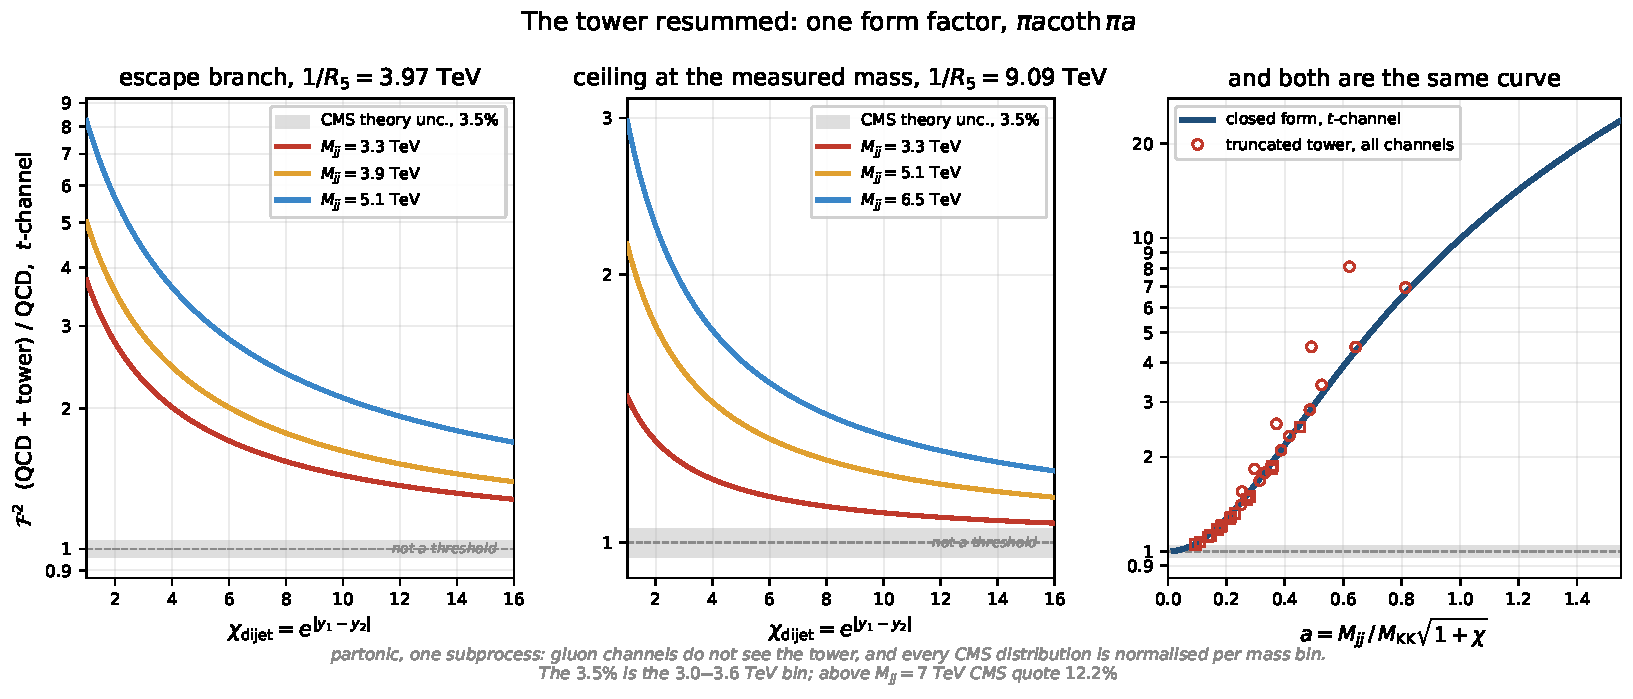
\includegraphics[width=\textwidth]{fig_tower.pdf}
\caption{\textbf{Why the angular distribution and not the mass spectrum --- and it is one
function.} The exact $t$-channel ratio $\mathcal F^2$ of \eqref{eq:resum}, with no truncation, no
width and no $\mathrm{BR}(G_n\to jj)$. At fixed dijet mass $|t|=M_{jj}^2/(1+\chi)$, so the effect
is largest where $\chi$ is smallest, which is exactly where $t$-channel QCD is weakest.
\emph{Left:} the branch that can also pay for Part~VI's escape from proton decay. \emph{Middle:}
the whole class, capped at the measured Higgs mass. \emph{Right:} why those two are the same
picture. $\mathcal F$ sees $M_{jj}$, $\chi$ and $M_{\mathrm{KK}}$ only through
$a=M_{jj}/M_{\mathrm{KK}}\sqrt{1+\chi}$, so every curve in the other two panels \emph{is}
$(\pi a\coth\pi a)^2$ and they collapse onto one line. The hollow markers are the superseded
all-channel calculation of \texttt{kk\_\allowbreak dijet\_\allowbreak lo.py} --- tower truncated,
widths on --- which meets the closed form to $1.4\,\%$ away from the tower and departs from it
upward only where the $s$-channel opens; that departure is exactly the part $\mathcal F^2$ does
not describe, and it is drawn rather than described. The grey band is the $3.5\%$ total
theoretical uncertainty \cite{CMSangular} quotes for its normalised $\chi_{\mathrm{dijet}}$ in the
$3.0$--$3.6$~TeV bin --- drawn to give the vertical axis a scale, \textbf{not as an exclusion
threshold}, which would need the full likelihood over correlated bins. \textbf{And the curves are
an over-estimate}: they are one subprocess at parton level, gluon-initiated ones do not see the
tower at all by the same five-momentum argument that removes it from $q\bar q\to gg$, and every
CMS distribution is normalised per mass bin. What the picture establishes is the size and the
shape --- which is a reason to do the recast, not a result of one. Drawn by
\texttt{make\_\allowbreak fig\_\allowbreak tower.py}.}\label{fig:tower}
\end{figure}

\noindent\textbf{And the published limit is not the one to read off.} \cite{CMSangular}'s
contact-interaction scenarios are stated to have colour-singlet couplings between quarks, while
the tower's operator is a colour octet, and the two interfere with QCD differently. The octet
carries the colour flow of one-gluon exchange, so in the $t$-channel it interferes at full
strength while the singlet does not, by $\mathrm{Tr}\,T^a=0$. That contraction is not the whole
story: for \emph{identical} quarks the crossed $t$--$u$ terms restore the singlet's interference
and its colour weight there is three times the octet's. Both are verified with explicit
generators in \texttt{colour\_\allowbreak octet\_\allowbreak recast.py}, and the simplest check
needs none of that algebra --- \cite{CMSangular} quotes $17$~TeV for destructive and $37$~TeV for
constructive interference, and a vanishing interference could not make the limit depend on the
sign. So which operator a given dataset constrains more tightly is not decidable from colour
factors: it turns on the flavour composition of the sample. What does follow is that the
published scale cannot be carried across. The translation is a calculation, not a rescaling, and
it is performed below.

\paragraph{The recast, and what one number of it may be quoted.} \cite{CMSangular} publish the
unfolded $\chi_{\mathrm{dijet}}$ distribution in seven mass bins together with a $77\times77$
correlation matrix and their own QCD NNLO + EW NLO prediction at \emph{both} of their scale
choices, so the Standard-Model baseline is theirs and only the relative deformation is ours. The
deformation is \eqref{eq:resum} in $t$ and $u$ alone --- no width, no $\mathrm{BR}(G_n\to jj)$ ---
folded with parton densities over every subprocess, and fitted with the scale choice profiled
between their two columns as a nuisance, because their own small tension below $4.8$~TeV moves
between them. Three things are checked before the fit is read. The hadron-level layer reproduces
CIJET's leading-order colour-octet interference to $0.2\,\%$ bin by bin, absolutely and in
picobarns, on a matching with no free factor. \cite{CMSangular}'s own NNLO put through this
$\chi^2$ gives $\chi^2/\mathrm{ndf}=0.81$. And, aimed at the published contact-interaction limit
for the standard colour-singlet operator --- and run on the mass range they set it on, $M_{jj}>
3.6$~TeV, which is not the full seven bins --- the machinery returns $17.5$ against their $17$~TeV
and $29.5$ against their $37$~TeV. On all seven it returns $20.5$ and $25.5$ instead, and the
difference is the point: a closure test has to close on the selection it is closing on.

\noindent\textbf{The statistic, written out, because a limit whose $\chi^2$ is only in the code is
not reproducible from the paper.} Let $d$ be the $77$ unfolded values, laid out in seven mass
blocks $B_m$ of sizes $(12,12,12,12,12,12,5)$, and let
\begin{equation}\label{eq:chisq}
\begin{aligned}
  t_i(M,a)\;&=\;\mathcal N_m\Big[(1-a)\,T_i^{\mu=m_{jj}}
             +a\,T_i^{\mu=\langle p_T\rangle}\Big]\big[1+\delta_i(M)\big],\\[2pt]
  \chi^2(M)\;&=\;\min_{a\in[0,1]}\;r^{\mathsf T}C^{-1}r\,,\qquad r=d-t(M,a)\,,
\end{aligned}
\end{equation}
with $\delta_i(M)$ the tower's deformation of \eqref{eq:resum} in $t$ and $u$, and $\mathcal N_m$
renormalising each mass block to unit area, as the measurement is. The nuisance $a$ interpolates
linearly between \cite{CMSangular}'s two published scale choices and is profiled by minimisation
with \emph{no} penalty term --- it is a choice between two of their own columns, not a measured
parameter, so a Gaussian prior on it would be invented. The quoted number is the $M$ at which
$\chi^2(M)-\chi^2_{\mathrm{SM}}$ falls through $3.84$, with $a$ re-profiled at every $M$.

\noindent\textbf{That is an SM-referenced criterion and not Wilks' $95\,\%$ point, and the
difference is not academic here.} Wilks measures $\Delta\chi^2$ from the \emph{minimum}, which
equals $\chi^2_{\mathrm{SM}}$ only if the Standard Model is the best fit --- and it is not. On the
full seven bins $\chi^2$ bottoms out at $58.46$ at $1/R_5=16.0$~TeV against $62.57$ for no tower at
all: \textbf{the data weakly prefer a finite tower}, by $\Delta\chi^2=4.12$. That is a nominal
$2.0\,\sigma$ for one degree of freedom and it should be read as almost nothing, for a reason the
same scan supplies: restrict to $M_{jj}>3.6$~TeV, which drops the $3.0$--$3.6$~TeV bin, and the
preference collapses to $\Delta\chi^2=0.29$. \emph{The preference is \cite{CMSangular}'s own
$2.0\,\sigma$ local excess in that bin, seen through our template, not information this recast
adds.} There is no look-elsewhere correction here, no detector-level likelihood, and the
$\theta=1/M^2\ge0$ boundary makes the asymptotic distribution a Chernoff mixture rather than a
$\chi^2_1$; we report the number because hiding it would be worse, and claim nothing from it.

\noindent\textbf{So the criterion is varied instead of defended}, and the spread is what the reader
should look at:
\begin{center}\small
\rowcolors{2}{white}{softgrey}
\begin{tabular}{llll r}
\toprule
\rowcolor{hdrblue!10}what is varied & points & covariance & criterion & $1/R_5$ [TeV]\\
\midrule
--- (the reference point) & $70$ & raw $C$ & $\Delta\chi^2_{\mathrm{SM}}=3.84$ & $11.20$\\
reference of $\Delta\chi^2$ & $70$ & raw $C$ & $\Delta\chi^2_{\min}=3.84$ & $12.18$\\
reference and one-sidedness & $70$ & raw $C$ & $\Delta\chi^2_{\min}=2.71$ & $12.60$\\
scale profiled \emph{discretely} & $70$ & raw $C$ & $\Delta\chi^2_{\mathrm{SM}}=3.84$ & $11.19$\\
normalisation projected out & $70$ & $JCJ^{\mathsf T}$ & $\Delta\chi^2_{\mathrm{SM}}=3.84$ & $11.29$\\
NNPDF3.1 \cite{NNPDF31}, \cite{CMSangular}'s baseline & $70$ & raw $C$ & $\Delta\chi^2_{\mathrm{SM}}=3.84$ & $11.62$\\
CT14nlo \cite{CT14} & $70$ & raw $C$ & $\Delta\chi^2_{\mathrm{SM}}=3.84$ & $11.46$\\
\midrule
\textbf{quoted in \eqref{eq:tulimit}} & $\mathbf{77}$ & raw $C$ & $\Delta\chi^2_{\mathrm{SM}}=3.84$ & $\mathbf{10.86}$\\
\bottomrule
\end{tabular}
\end{center}
\noindent The columns matter: the spread is \emph{not} all statistical redefinition. Seven of the
eight rows sit on the same $70$-point $\chi^2$ and differ only in what they vary; the last drops
that choice instead and keeps all $77$, which is where the extra $3\,\%$ comes from. Nothing in the table mixes two changes at once.

\noindent Three of those rows answer objections rather than tune. The discrete row profiles over
\cite{CMSangular}'s two scale columns \emph{without} interpolating: their difference is larger than
the usual six-point scale variation, so the interpolants between them are not themselves computed
predictions, and a limit leaning on one would have bought freedom rather than measured it. It gives
$11.19$ against $11.20$, so the continuous nuisance buys nothing and is validated empirically. The
two parton-density rows answer the objection that CT10nlo is not \cite{CMSangular}'s baseline and
that at $M_{jj}=5$--$8$~TeV we sit at high $x$, where the $uu\!:\!ud\!:\!dd\!:\!qg\!:\!gg$ mixture
is set-dependent and the deformation touches only quark channels: on the $70$ points of the table,
NNPDF3.1 gives $11.62$~TeV and CT14nlo $11.46$ against CT10nlo's $11.20$ --- \textbf{a spread of
$3.7\,\%$, with CT10nlo the weakest of the three}. \textbf{And the same comparison repeated in the
configuration that actually produces \eqref{eq:tulimit}} --- all $77$ points --- gives $11.27$,
$11.11$ and $10.86$: the same $3.7\,\%$ spread, the same ordering, CT10nlo still weakest. So
staying on CT10nlo is the conservative choice in both, and the systematic does not depend on which
of the two $\chi^2$ the comparison is made in. \emph{Two earlier versions of this sentence got that
number wrong in opposite directions, both by comparing across configurations: first $3.8\,\%$ from
NNPDF3.1 at $70$ points against the quoted $10.86$ at $77$, then ``$1.4\,\%$'' from a mixture of
both. Quoted consistently it is $3.7\,\%$ either way.} CT10nlo also stays in the CIJET
control, because it is the set their grid was generated with and a control run with another set is
not a control. The projected row is explained below. Every criterion lands above the quoted
$10.86$~TeV, which is therefore the weakest of them and the one it is safe to carry.

\noindent\textbf{And that $3.7\,\%$ is the spread \emph{among} fits, not the uncertainty of what
they assume.} All three sets are fitted to overlapping data under the same hypothesis --- that the
proton has no substructure at these scales --- and this recast's whole sensitivity sits at high $x$
and high $M_{jj}$, which is where that hypothesis is least constrained and where a mismodelled
parton density and a four-quark contact operator produce the \emph{same} signature. That
degeneracy is why compositeness searches are hard, and it is not covered by varying the set. It
does not move \eqref{eq:tulimit} --- nothing here can say by how much it would --- but a reader
should know it is a floor under the systematic and not something the three rows above have
measured.


\noindent Three facts about $C=\sigma\sigma^{\mathsf T}\!\circ R$ are measured rather than assumed,
and one of them corrects an earlier claim of ours. $C$ has \emph{full rank} $77$, condition number
$1.2\times10^4$: no pseudoinverse is used or needed anywhere. The data do obey the unit-area
constraint block by block to $2\times10^{-5}$ --- \emph{but $C$ does not know it}: on the constraint
direction $w$ (the bin widths inside a block) $w^{\mathsf T}Cw$ runs from $0.13$ to $0.83$ of that
block's own scale rather than vanishing, so the published matrix is not the covariance of the
normalised distribution alone. An earlier version of this work dropped the last bin of each block
and justified it as the remedy for a singular matrix; that justification was wrong, and the drop is
a \emph{choice}. So it is made both ways: on $70$ points the fit gives $11.20$~TeV and on all $77$
it gives $10.86$~TeV, a spread of $3.2\,\%$, and what is quoted is the weaker. On
\cite{CMSangular}'s own contact-interaction mass range those two give $13.95$ and $14.10$~TeV, a
spread of $1.1\,\%$ --- there the weakest reading is neither of them but the projected covariance
below, at $13.75$~TeV, which is why that is the number quoted for that selection.

\noindent\textbf{And that full rank has a documentary explanation which is also the sharpest
objection to this fit, so it is stated in the record's own words.} The \textsc{hepdata} record
describes the matrix as ``the correlation matrix of the maximum likelihood estimators of the signal
strength modifiers'', obtained ``after the fit to the data'' --- \emph{not} as the covariance of the
normalised unfolded points. If the unit-area normalisation is applied \emph{after} that fit, then
$d_i=x_i/\sum_j w_jx_j$ mixes bins and the covariance of $d$ is $JCJ^{\mathsf T}$ with
$J_{ij}=\delta_{ij}-d_iw_j$, which does have the constraint direction as an exact null mode --- so
for that row, and only that row, one bin per normalised block is removed and the $\chi^2$ is
evaluated on the resulting $70$-dimensional non-singular representation. There too no pseudoinverse
is used: on the raw matrix because none is needed, here because the singular direction is projected
out by construction rather than inverted through. A
reader is entitled to ask why $\sigma_i\sigma_jR_{ij}$ may be used when the two objects may live in
different parametrisations, and we cannot settle it from the record: it is not documented either
way. What can be done is to compute the limit \emph{under the unfavourable reading} and see whether
the question has any numerical force. It does not: through $JCJ^{\mathsf T}$ the limit is
$11.29$~TeV against the $11.20$ of the raw matrix, eight parts in a thousand, and in the direction
that strengthens it. \textbf{The objection is real and its consequence is below a per cent}, which
is a better answer than an argument would have been. The result is
\begin{equation}\label{eq:tulimit}
  \frac{1}{R_5}\;>\;10.86\ \text{TeV}\,,
\end{equation}
and $13.75$~TeV on the mass range \cite{CMSangular} themselves restrict their contact-interaction
limit to, $M_{jj}>3.6$~TeV. That the number \emph{rises} when the $3.0$--$3.6$~TeV bin is dropped
is worth saying: that bin carries their largest local excess, $2.0\sigma$, in the same direction
our signal would push, so the limit is not leaning on the one place the data are least quiet. Figure~\ref{fig:chi2} draws the profile those criteria summarise, and adds the one thing a table cannot: where the model's own allowed scales fall on it.

\begin{figure}[t]
\centering
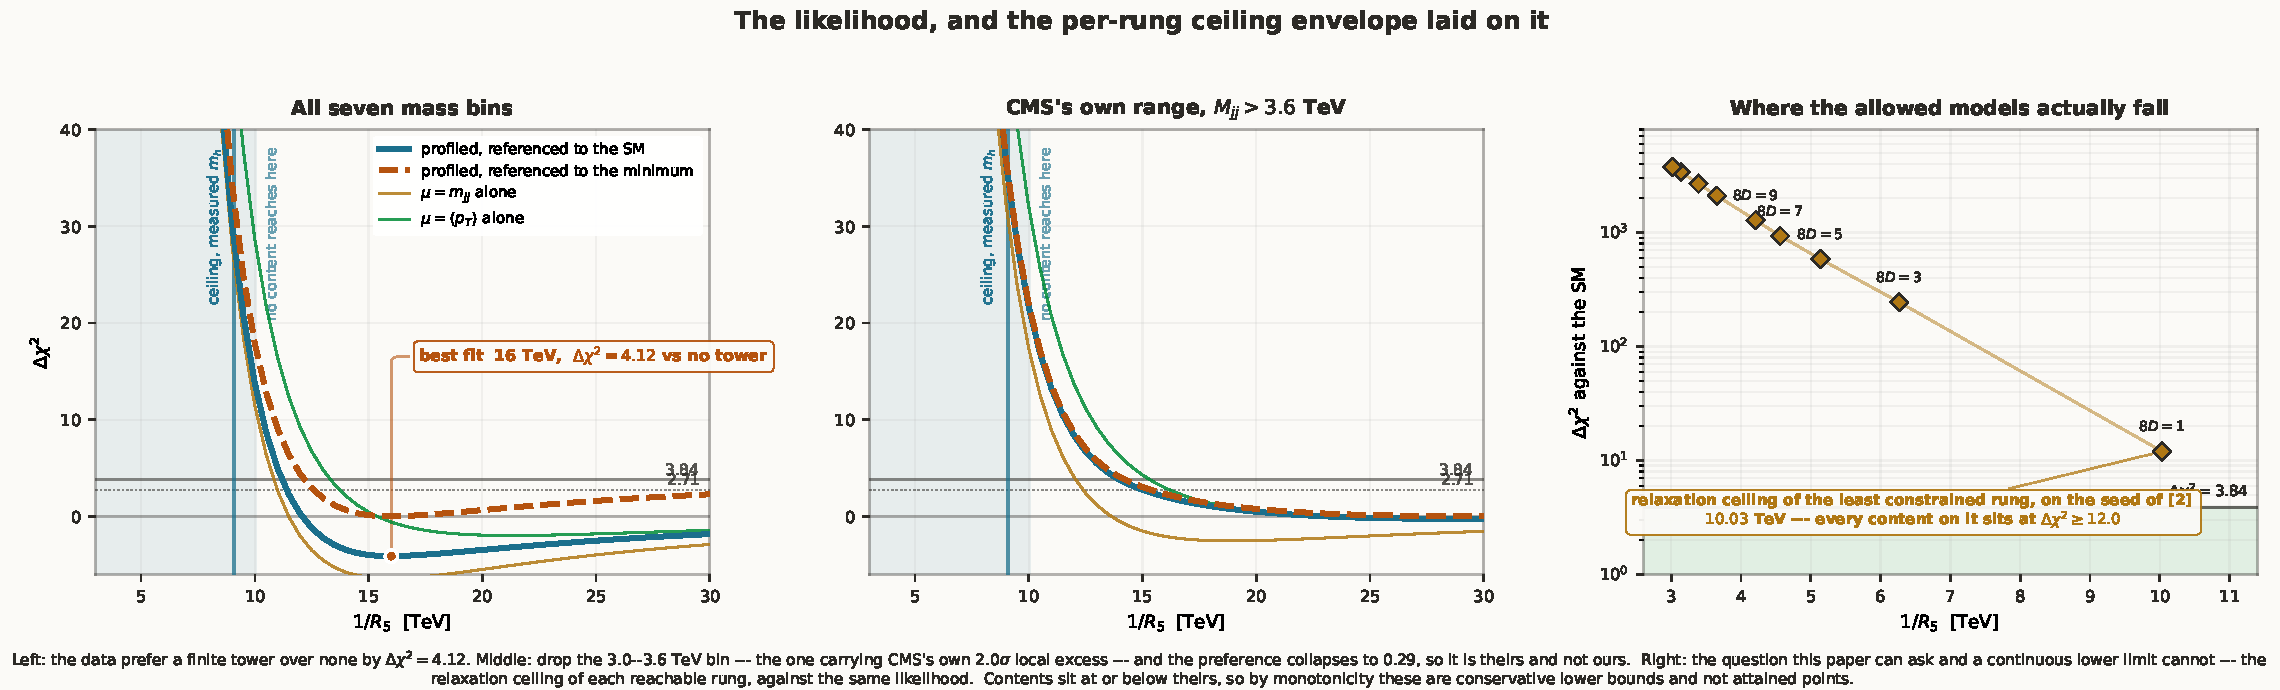
\includegraphics[width=\textwidth]{fig_chi2.pdf}
\caption{\textbf{The likelihood, and the per-rung ceiling comb laid on it.} The recast $\chi^2$ of
\eqref{eq:chisq} against $1/R_5$, with both references drawn --- solid against the Standard Model,
which is what \eqref{eq:tulimit} uses, and dashed against the \emph{minimum}, which is what Wilks'
$95\,\%$ point actually means. They differ because the Standard Model is not the best fit.
\emph{Left, all seven mass bins:} the curve bottoms out at a \textbf{finite} $1/R_5=16$~TeV,
$\Delta\chi^2=4.12$ below no tower at all --- a nominal $2.0\,\sigma$ for one degree of freedom.
The two thin curves are \cite{CMSangular}'s two scale choices taken separately, not interpolated:
they bracket the profiled result and show the same shape, so the minimum is not an artefact of the
nuisance. \emph{Middle, the same on $M_{jj}>3.6$~TeV}, which drops the $3.0$--$3.6$~TeV bin: the
minimum flattens and the preference collapses to $0.29$. \textbf{So the preference is
\cite{CMSangular}'s own $2.0\,\sigma$ local excess in that one bin, seen through our template, and
not information this recast adds} --- which is why no significance is claimed from it.
\emph{Right, the question a continuous lower limit cannot ask.} The diamonds are the per-rung
ceilings of \S\ref{sec:ceiling}, \eqref{eq:slope} --- the \emph{largest} $1/R_5$ the integer
programme allows at each quantised $8D$ --- read against the same likelihood, with
$\Delta\chi^2$ on a logarithmic axis because \emph{it} is what spans decades: the teeth themselves
run only from $10.03$ down to $3.02$~TeV, while their $\Delta\chi^2$ runs from $12.0$ to some
thousands. \textbf{They are relaxation ceilings and not attained contents}: the $8D=1$ diamond sits at
$10.03$~TeV while the lattice reaches only $10.01$ ---both on the seed \cite{KM25} print--- and a
content sits at or below its rung's
ceiling on the discrete set the arithmetic comb allows. \textbf{That does not weaken the reading;
it is what makes it a bound.} Since $\Delta\chi^2$ decreases monotonically with $1/R_5$ across
this range --- measured, and true up to $15.5$~TeV, well past the highest tooth --- a content at or
below its ceiling sits at or \emph{above} that ceiling's $\Delta\chi^2$. So each diamond is a
conservative lower bound on the $\Delta\chi^2$ of every content on its rung, and the minimum over
the diamonds bounds the minimum over all contents from below without needing any diamond to be
attainable at all. The band below
$\Delta\chi^2=3.84$ is \textbf{empty}: the comb's highest tooth is the $8D=1$ ceiling at
$10.03$~TeV on the seed \cite{KM25} print, and even that sits at $12.0$. \textbf{That panel is read on the $77$-point $\chi^2$},
the one \eqref{eq:tulimit} is quoted from, and not on the $70$-point curve the other two panels
draw --- which is why its $8D=1$ point does not lie on the solid line to its left. On that curve
the same tooth would read $13.4$; the weaker of the two is the one quoted. Drawn by
\texttt{make\_\allowbreak fig\_\allowbreak chi2.py} from \texttt{scan\_\allowbreak mkk.py}'s and
\texttt{ceiling\_\allowbreak ilp.py}'s archived runs.}\label{fig:chi2}
\end{figure}

\noindent\textbf{And that last panel is the question this paper can ask and a continuous lower
limit cannot.} A limit says ``above $10.86$~TeV''. But $1/R_5$ is not continuous here: $8D$ is an
odd integer on the seed \cite{KM25} print, so the per-rung ceilings form a \emph{comb} of their own, and
\eqref{eq:slope} gives its teeth ---
$10.03$~TeV at $8D=1$, then $6.27$, $5.14$, $4.56$, falling to the Lambert asymptote.
\textbf{And it is not the arithmetic comb of \S\ref{sec:pred}}: that one lives \emph{inside}
a rung, with an exact step in $M^2$, and is the set of masses that rung reaches; this one has
a single tooth per rung, and the tooth is the most that rung reaches rather than all of it. A
content may sit anywhere at or below its own. Reading the
recast at each tooth instead of at an arbitrary mass gives
\begin{keyeq}
\begin{equation}\label{eq:combchi}
  \min_{k\ \mathrm{odd}}\ \Delta\chi^2\big(M_{\max}(k)\big)\;=\;12.0
  \qquad\text{at } 8D=1,\ 1/R_5=10.03\ \text{TeV,}
\end{equation}
\end{keyeq}
\noindent against a threshold of $3.84$; the next tooth is at $\Delta\chi^2=244$ and the escape
branch's best, $3.97$~TeV, beyond a thousand --- all three are $\Delta\chi^2$, not masses. \textbf{Two things about that number are choices and are made the
unfavourable way.} It is read on the $77$-point $\chi^2$ --- the one \eqref{eq:tulimit} is quoted
from because it is the weaker --- and not on the $70$-point one, which would give $13.4$ instead;
and the teeth are the \emph{truncated} per-rung ceilings, $10.034$~TeV at $8D=1$, rather than the
untruncated $10.037$, which sits three GeV higher and so a shade lower in $\Delta\chi^2$. Neither
is worth a decimal on its own; both are stated because a reader cannot otherwise tell which of
several available numbers was picked.

\noindent\textbf{And now the question that matters more than either: why does \emph{one} tooth
carry all of this?} Because the per-rung ceiling falls with $k$ --- $A_4$ cannot keep pace, its
cap per rung running $215,112,87,76,\dots$ per unit of $8D$ --- so the least-constrained tooth is
always the \emph{smallest} rung, and the smallest rung is $8D=1$ only because
Theorem~\ref{thm:eighths} says $8D$ is an odd \emph{integer} wherever its hypothesis is met, which
on the seed \cite{KM25} print it is. \textbf{So the margin behind
\eqref{eq:combchi} is not $12.0$ against $3.84$. It is the integrality of $8D$}, and that can be
measured rather than admired: at fixed $A_4$ the ceiling scales as $k^{-1/2}$, so a quantum half
as large would put the top tooth at $14.19$~TeV, where this recast returns
$\Delta\chi^2=-6.0$ --- \emph{below} the Standard Model, inside the region the data mildly prefer.
Halve the quantum and the conclusion does not weaken; it changes sign.

\noindent That is worth following one step further, because it ends somewhere specific and the
ending is not a weakness. On the seed \cite{KM25} print, $8D$ is odd because matter contributes
an even amount and the gauge sector an odd one. It is tempting to put that oddness down to a \emph{single half-integer} --- the
weight $\tfrac12$ of each $P_6=-1$ adjoint pair, against $2$ for each $P_6=+1$ pair --- but that is
not what carries it, and the distinction turns out to decide the whole chain. Over the $n_+=2$ and
$n_-=6$ pairs of the row that mixes them, the coefficient is $2n_++\tfrac12 n_-=4+3=7$: the
antiperiodic term contributes $3$, an \emph{integer}, and the oddness of the sum needs the periodic
term to be even at the same time. \textbf{Two conditions, not one, and neither weight decides
alone} (Figure~\ref{fig:ghosts}). The antiperiodic $\tfrac12$ is not read off \cite{KM25}'s eq.~(68) --- it is
\emph{inferred}, and by a fit that had a way to fail. Part~VI \cite{PartVI} builds all $48$ adjoint generators, reads $(q,P_5P_5',P_6)$
off each, and fits \emph{two} weights to \emph{three} coefficients: the \emph{two} rows with no
$P_6=-1$ pairs fix the periodic weight on their own, and they agree; the remaining row then forces
the antiperiodic one to be exactly $\tfrac12$, reproducing their $7$ as $2\times2+6\times\tfrac12$,
the split their text states and never derives. \textbf{But the redundancy is not where it matters.}
Three coefficients against two unknowns is overdetermined as a \emph{system}, and it is tempting to
report it as a test that could have failed. It could --- but only of the periodic weight, which is
the one both spare rows constrain. The antiperiodic weight is fixed by one equation and checked by
none. What agrees is not what decides.

\begin{figure}[t]\centering
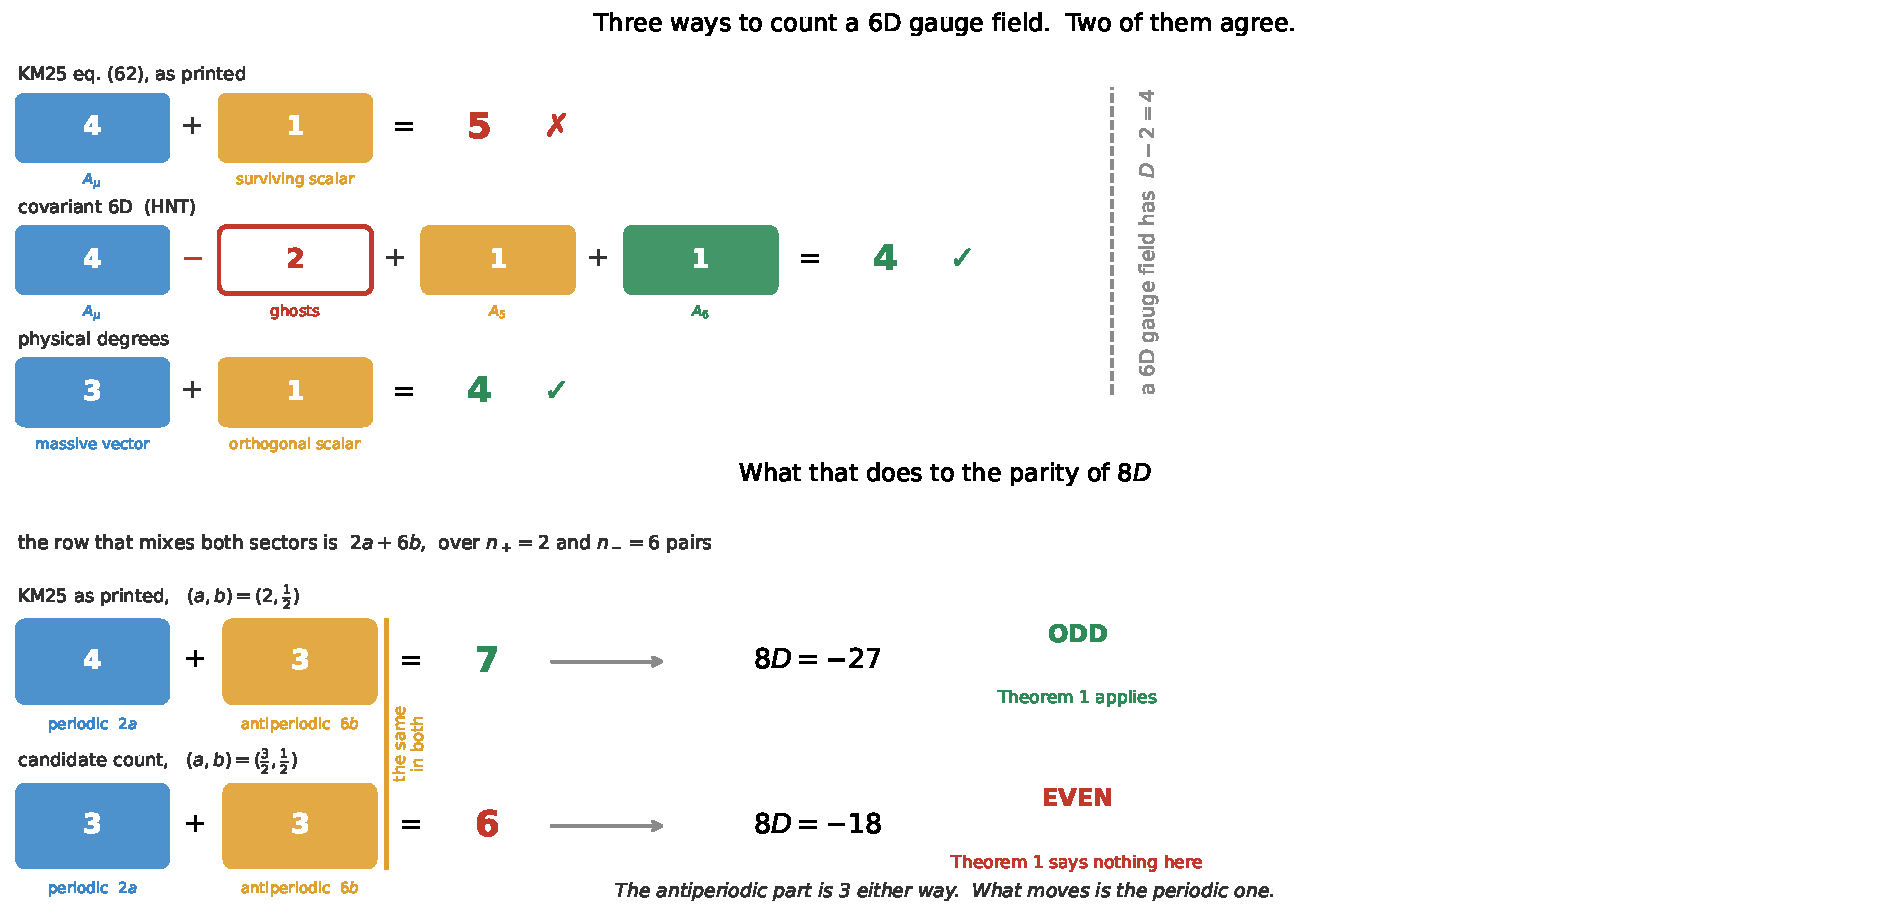
\includegraphics[width=\textwidth]{fig_ghosts.pdf}
\caption{\textbf{Where the parity comes from.} \emph{Top:} three ways to count the degrees of freedom of a six-dimensional gauge field. \cite{KM25} take $4$ for $A_\mu$ and $1$ for the surviving scalar; the covariant six-dimensional count of \cite{HNT} subtracts the two ghosts and keeps both extra-dimensional components, consistent with \cite{HY04}'s general $-(D-2)$ rule; the physical count uses the three polarisations of a massive vector. Two of the three give $D-2=4$, and the one that does not is the one this paper inherits. \emph{Bottom:} what that does to the row mixing the two $P_6$ sectors, whose coefficient is $2a+6b$ over $n_+=2$ and $n_-=6$ pairs. The antiperiodic part is $6\times\tfrac12=3$ either way --- an \emph{integer}, and it does not move. What moves is the periodic part, from $4$ to $3$, and with it the parity: $7$ against $6$, hence $8D=-27$ against $-18$. So the parity change cannot be put down to the antiperiodic half-integer alone --- the number \S\ref{sec:open} used to name as the open one: what changes is the parity character of the complete mixed coefficient $2a+6b$. The figure is drawn through the same five-coordinate map as the text, and refuses to draw at all unless it returns the published $-27$.}\label{fig:ghosts}
\end{figure}

\noindent \textbf{And then the half does not survive, which is the part worth understanding.} The
gauge weight --- written $\omega_g$, because $W$ is already the stability functional of
\S\ref{sec:ceiling} and the Lambert branch, and three objects to a letter is one too many ---
is $\omega_g=2n_++\tfrac12 n_-$ over the $P_6=\pm1$ adjoint pairs, and a census of all
$4096$ admissible diagonal assignments returns, with no counterexample, $n_-=2m$ --- where $m$
counts the indices doubly flipped relative to the Wilson-line pair. So
$\omega_g=2n_++m$ \emph{is an integer}, and it is odd exactly when $m$ is. In \cite{KM25}'s assignment
$m=3$, and the three indices that make it up are the colour indices of their eqs.~(78)--(79).
\emph{So what makes $8D$ odd is not a half at all: it is the parity of a count of colours.} The
$\tfrac12$ is the bookkeeping that counts each pair once, and because pairs come in twos it always
reconstitutes an integer. The chain is then: $m=3$ is odd, so $\omega_g$ is odd, so $8D$ is odd, so
$|D|\ge\tfrac18$, so $1/R_5$ is capped, so the class is finitely testable --- and the ceiling this
paper computes is that fact read at the other end. \textbf{Every link of that chain is sound; its
first link is inherited.} It begins with the weights $(2,\tfrac12)$ read off \cite{KM25}, and
\S\ref{sec:open} shows what the chain does if they are $(\tfrac32,\tfrac12)$ instead: it does not
break, it moves down one rung.

\noindent \textbf{One link in that chain is inferred and not derived, and the difference is one of
direction.} What Part~VI establishes independently is the \emph{table}: over the $48$ adjoint
generators, $(q,P_5P_5',P_6)$ is group theory and cannot move, which rules out any error in
\cite{KM25}'s multiplicities. What it does \emph{not} establish is the weights --- and it is worth
being exact about which of the two, because ``three coefficients, two unknowns, overdetermined''
does not mean what it sounds like here. \textbf{Two} of the three rows contain no $P_6=-1$ pair at
all, so each fixes the first weight on its own, and their agreement \emph{is} the redundancy.
\textbf{One} row contains the $P_6=-1$ pairs, so the second weight is fixed by a single equation
with nothing to check it against. \emph{So the redundancy tests the periodic weight and only that
one.}

\noindent And it is worth saying which of the two decides, because an earlier version of this
paragraph had it backwards. The row that mixes them is $2n_++\tfrac12 n_-$, and for that to come
out odd \textbf{two} things must hold at once: the periodic part even \emph{and} the antiperiodic
part odd. The antiperiodic part is $6\times\tfrac12=3$, odd either way, so it is safe. The periodic
part is the one a ghost subtraction would move, from $4$ to $3$. \emph{So the redundancy tested
precisely the weight that decides, and tested it in the one direction that was never in doubt.}
And in either case the inference
runs from their numbers back to the weights, not from the geometry forward to their numbers. The causal order is: six-dimensional field content $\to$ mode decomposition $\to$
weights $\to$ coefficients, and every route in this series enters that chain at the right-hand end.
\textbf{So $(2,\tfrac12)$ is what the coefficients require, not what the compactification predicts},
and no computation anywhere in Parts~I--VII derives it the other way. What would: a Coleman--Weinberg
sum over the six-dimensional Kaluza--Klein tower with these orbifold parities, computing the weight
of a $P_6=-1$ pair from its antiperiodic moding rather than reading it off. That is a standard
calculation and it is not done here; \S\ref{sec:open} carries it. Everything downstream of the
weights is proved.

\noindent \textbf{An attempt to close it forward, and why it failed --- which is worth recording
because the failure is instructive.} \cite{HY04} state their counting rule in words: the potential
is $[\text{fermionic d.o.f.}-\text{bosonic d.o.f.}]$ times the potential of one degree of freedom,
which for gauge plus ghosts is $-(D-2)$; and their eq.~(3.10) gives the one-d.o.f. adjoint
potential as weight $\tfrac12$ per charge pair, with one pair at $c=2$ and two at $c=1$ by their
eq.~(3.8). At $D=5$ that returns their own eq.~(3.20), $(\tfrac32,3)$. Carried to $D=6$ it returns
$(2,4)$, the periodic part of \cite{KM25}'s eq.~(68), and we briefly took that for an out-of-sample
derivation. \textbf{It is not one.} In six dimensions $D-2=4$ coincides numerically with the number
of $A_\mu$ components, which is four in \emph{every} dimension; the agreement therefore does not
distinguish the two bookkeepings, and in five dimensions --- where they differ, $3$ against $4$ ---
it is $D-2$ that \cite{HY04} use. Worse, $D-2$ is the total over \emph{both} parity sectors, and
assigning it whole to the periodic one is precisely the step that a second parity makes illegal.
So the periodic weight remains inferred, and the caveat above stands unweakened.

\noindent \textbf{And the same arithmetic, read the other way, is a live question about
\cite{KM25}'s bookkeeping that this paper cannot settle and should not hide.} Their eq.~(62)
assigns $N=4$ to $A_\mu$ and, after removing the Goldstone combination, $N=1$ to the surviving
$A_{5,6}$ scalar. With our own generator table --- one pair at $c=2$, two at $(c{=}1,s{=}{+}1)$,
and two $P_6{=}{+}1$ plus six $P_6{=}{-}1$ at $(c{=}1,s{=}{-}1)$ --- those two numbers reproduce
eq.~(68) exactly: $2$, $4$, and $(2\times4+6\times1)/2=7$. \textbf{But $4+1=5$, while a
six-dimensional gauge field has $D-2=4$ physical polarisations.} \cite{HNT} do the covariant count
on $T^2/\ZZ_2$ and state it plainly --- ``the mass matrix for ghost fields is the same as that for
$A_\mu$'', so $A_\mu$ and ghosts give $4-2=2$, and the two extra-dimensional components give $2$
more, totalling four. Their orbifold is not this one --- \cite{KM25} use the product
$S^1/\ZZ_2\times S^1/\ZZ_2$, with two independent reflections --- so what they fix is the total,
not how a second parity divides it. Carried over to the product orbifold at $R_5\gg R_6$, a
parity-resolved covariant count \emph{suggests} that the four split $3$ on the $P_6{=}{+}1$ side
and $1$ on the other, rather than $4$ and $1$. Were that right, substituting $4\to3$ would turn
eq.~(68) into $(\tfrac32,3,6)$, the gauge sector's $8D$ would be $-18$ rather than $-27$,
\emph{even}, and \textbf{the hypothesis of Theorem~\ref{thm:eighths} would not be satisfied} ---
which is a different statement from the theorem failing, and the difference is the whole point. \textbf{We do not assert that \cite{KM25} are wrong}: no
Faddeev--Popov determinant is displayed in their one-loop bookkeeping, but a gauge-fixing term is,
and a cancellation could be implicit in how their spectrum is built. What settles it is a
computation this paper does only in part (\S\ref{sec:open}) --- the background-gauge determinant for a \emph{single} charged
adjoint orbit, $\tfrac12\log\det\Delta_{A_\mu}+\tfrac12\log\det\Delta_{A_5}
+\tfrac12\log\det\Delta_{A_6}-\log\det\Delta_{\mathrm{FP}}$ at $R_5/R_6\to\infty$, which needs
neither $\su7$ nor forty-eight components. \emph{Until that is done, every consequence here that needs the published gauge base point inherits
this question --- which is not every theory-side scale, since the asymptote \eqref{eq:rinf} carries
no gauge quantity at all --- and it is a sharper question than the anchor residual it sits beside.}

\noindent \textbf{And the exposure is narrower than ``one inferred number'' makes it sound, which
is worth saying because it cuts the other way.} The natural worry --- what if the weight is not
exactly $\tfrac12$? --- is the wrong question. Since $n_-=2m$ always, the gauge weight is
$\omega_g=2n_++2b\,m$. \textbf{An earlier version of this paragraph read that as a robustness
result about $b$, and had the emphasis exactly backwards.} On the row that carries the physics,
$n_+=2$ and $n_-=6$, the whole question is this:
\begin{keyeq}
\begin{equation}\label{eq:twoparities}
  \begin{aligned}
    \omega_g\;&=\;2a+6b\;=\;(2a)+3\,(2b)\,,\\[2pt]
    \omega_g\ \text{odd}\;&\iff\;(2a)+(2b)\ \text{odd}\qquad(\text{for }2a,2b\in\ZZ)\,.
  \end{aligned}
\end{equation}
\end{keyeq}
\noindent Both weights enter, symmetrically, and neither decides alone:
\[
  (a,b)=\Bigl(2,\tfrac12\Bigr):\ 4+3=7\ \text{odd};\qquad
  (a,b)=\Bigl(\tfrac32,\tfrac12\Bigr):\ 3+3=6\ \text{even}.
\]
The antiperiodic weight is the \emph{same} in both, and the parity still flips. So the chain does
not hang on $b$, and it was never $b$ that was in danger: what \S\ref{sec:open} puts in question
is $a$, and \eqref{eq:twoparities} says why that is enough on its own.
Measured in \texttt{gauge\_\allowbreak weight\_\allowbreak origin.py} and
\texttt{gate\_\allowbreak km\_\allowbreak ghosts.py}. What \S\ref{sec:open} records
is a different and narrower gap: no \emph{published} computation tests that weight. Every anchor a
curvature can be checked against sits at $B=0$, where the parity-weighted and parity-blind moments
coincide; the parity-split results that \emph{do} carry an antiperiodic sector --- \cite{CCD24}'s
among them --- live at the value rung $p=5$ and never reach the curvature. Our own
chain has two legs; the outside world has none. A reader deciding how much weight
\eqref{eq:combchi} can bear should know that this is where it lives --- not in the statistics. \textbf{So it is not that the allowed region is partly disfavoured: no bulk
content the arithmetic of the seed \cite{KM25} print permits reaches any $1/R_5$ at which this
recast's $\Delta\chi^2$ falls below $12.0$.} The caveats of the previous paragraphs all still apply to that number, and none of the
\emph{quantified} collider-side variations above comes near the factor of three and a half in
$\Delta\chi^2$ that erasing the margin would take --- the unmeasured NLO deformation and the
theory-side anchor residual sit outside that statement, and are not claimed to be small. And it is a
nominal figure from a Gaussian recast, not a $CL_s$, and it is stated as one. What makes it worth
stating is that it is the two halves of this paper meeting: the integer programme says which
scales exist, and the likelihood says what the data think of them.
\paragraph{And the channel that was left out, put back.} \eqref{eq:tulimit} dresses $t$ and $u$
only, and the reason given for that is good --- there the resummed propagator is real, so neither
the width nor $\mathrm{BR}(G_n\to jj)$ enters, and the limit does not depend on exotic masses the
model never fixes. \textbf{But that argument does not show the omission is conservative}, and it
is not: amplitudes interfere, and in $q\bar q\to q\bar q$ the timelike term can add to the $t/u$
deformation or subtract from it. So it is computed. Only two matrix elements carry a timelike
gluon --- $q\bar q\to q\bar q$, through its $s$ piece and the $s$--$t$ interference, and
$q\bar q\to q'\bar q'$, which is pure $s$; the gluon final states stay undressed by the same
five-momentum argument of \cite{DMN01} used above. The pole is regulated by the \emph{total} width
$\Gamma_{\mathrm{tot}}=\Gamma_{q\bar q}+\Gamma_{\mathrm{exotic}}$ with
$\Gamma_{q\bar q}/M=2\alpha_s$ and $\Gamma_{\mathrm{exotic}}\ge0$ unknown, so
$\Gamma_{\mathrm{exotic}}$ is profiled rather than chosen.

\noindent Two things come out, and the first makes the second easy. \emph{The shift shrinks as the
width grows} --- at $1/R_5=9.09$~TeV the ratio to QCD moves by $-0.47\,\%$ at
$\Gamma_{\mathrm{exotic}}=0$ and by only $-0.18\,\%$ at $\Gamma_{\mathrm{exotic}}/M=1$ --- so the
profile over $\Gamma_{\mathrm{exotic}}\ge0$ is bounded at the \emph{boundary}, and the worst case
is a width we know rather than one we have to scan to infinity. And \emph{the sign is negative},
as the objection suspected: dropping the $s$ channel was not conservative. What it is worth is
small. That $-0.47\,\%$ on the ratio is $-6\,\%$ on the \emph{deformation}, ratio minus one, which
is what the fit sees; recomputing the limit rather than rescaling it --- the deformation does not
scale exactly, the bins are correlated and the scale is profiled --- gives
\begin{equation}\label{eq:stu}
  \frac{1}{R_5}\Big|_{s+t+u,\ \Gamma_{\mathrm{exotic}}=0}=12.86\ \text{TeV}
  \qquad\text{against}\qquad
  \frac{1}{R_5}\Big|_{t/u}=12.99\ \text{TeV}\,,
\end{equation}
both at leading order on the same grid, so that the $-1.03\,\%$ between them is the $s$ channel and
nothing else. That suggests an $\mathcal{O}(0.1~\text{TeV})$ effect on \eqref{eq:tulimit}, and both
readings stay above $10.03$ either way; the exact shift needs the final $77$-bin pipeline rerun with
$s+t+u$, and carrying a leading-order per cent across to it is the rescaling this paper declines to
do everywhere else.
\textbf{So the omission is real, its direction is the unfavourable one, and its size is one per
cent} --- which is worth saying in that order. Measured in
\texttt{s\_\allowbreak channel\_\allowbreak width.py}, whose first control rebuilds the whole
calculation from scratch and, with the $s$ channel switched off, reproduces the archived $t/u$
deformation to $6\times10^{-16}$; without that the difference could not be attributed to the
channel rather than to the rebuild.


\paragraph{And what that number is not.} It is \textbf{not} a CMS-equivalent $95\,\%$ CL
exclusion, and the difference is not pedantry. \cite{CMSangular} set limits with detector-level
Poisson likelihoods, profiled nuisance parameters and an asymptotic $CL_s$ construction; this is a
Gaussian $\chi^2$ over their published particle-level covariance with one nuisance. The two
closure benchmarks measure that gap --- and they measure it \emph{differently}, $1.03$ on the
destructive sign against $0.80$ on the constructive one, because those two are not two draws from
one uncertainty. \textbf{Running the same closure on the \emph{expected} limits says which of the
two explanations that is.} An Asimov dataset --- \cite{CMSangular}'s own Standard-Model prediction
put in place of their data, at its best-fit scale, with the covariance untouched --- returns $20.0$
and $29.0$~TeV against their published expected $18$ and $34$, that is $1.08$ and $0.85$. Those
are the observed ratios again to within five points. \emph{So the gap is a property of the method
and not of a fluctuation in this particular dataset}, which is what an observed-only closure could
never have separated. It places the \emph{benchmark-dependent closure discrepancy} on the matched
contact-interaction selection at the ten to twenty per cent level in $\Lambda$, and larger over all
seven bins --- which is not a bias estimated over an ensemble, because no
ensemble was built; it is the disagreement measured on two templates, its size depends on which
selection it is measured on, and it is not a band that
transfers to \eqref{eq:tulimit}. Changing the sign of the interference changes the shape, can cancel against the
$1/\Lambda^4$ term and moves which bins dominate; read as coefficients of $1/\Lambda^2$ the same
two ratios become $0.94$ and $1.56$, which is template dependence and not a calibration.
\textbf{So they are diagnostics, and this paper does not turn them into a band on
\eqref{eq:tulimit}.} What may be said is that the recast finds enough tension that closing the
likelihood properly is the priority, and that $3.97$~TeV sits a factor of three below where the
recast loses sensitivity --- with no width and no $\mathrm{BR}(G_n\to jj)$ anywhere in it, which is
the whole reason for using the spacelike channels alone. What is \emph{not} settled is the
ceiling: $10.86$ and $13.75$ both clear $9.09$ and $10.03$~TeV, but a nominal recast sensitivity is
not the instrument that may retire a model, and \S\ref{sec:open} says what would be. Measured in
\texttt{hadronic\_\allowbreak chi.py}, \texttt{cijet\_\allowbreak control.py},
\texttt{fetch\_\allowbreak hepdata.py}, \texttt{cms\_\allowbreak ci\_\allowbreak closure.py} and
\texttt{scan\_\allowbreak mkk.py}, with parton densities from \cite{CT10} through
\cite{LHAPDF} and the contact-operator coefficients from \cite{CIJET}.

\begin{keyeq}
So the two calculations already cross \emph{numerically}: the algebraic ceiling of
\S\ref{sec:ceiling} approaches $1/R_5$ from \emph{above}, at $9.09$~TeV, and the nominal collider
sensitivity from \emph{below}. Promoting the second to an experimental lower bound requires the
detector-level likelihood, and \S\ref{sec:open} says so; the crossing is what makes that worth
doing rather than a result of having done it. \textbf{And read at the comb rather than at a
continuous scale, the crossing is not marginal}: \eqref{eq:combchi} puts every reachable
$1/R_5$ at $\Delta\chi^2\ge12.0$ --- on the seed \cite{KM25} print, whose comb this is. The
candidate seed's highest tooth is \emph{lower}, $7.38$~TeV, and $\Delta\chi^2$ falls
monotonically with $1/R_5$ across this range (Figure~\ref{fig:chi2}), so that branch is more
disfavoured and not less --- though it has not been read tooth by tooth. What is already true without any of it is the asymmetry:
every published constraint on a compactification scale bounds from below, and a lower bound alone
can never exclude a class --- the scale can always be raised. It is the ceiling that makes the
question finite, and the quantisation that makes it sharp.
\end{keyeq}

\bridge{The dictionary is derived, the one free parameter is named, the measurement has been
identified and then made, and the comb has been read against it --- which leaves only the
arithmetic instrument itself to be checked against someone else's table.}

% ===================================================================
\section{A second anchor}\label{sec:anchor}

Part~VI has one anchor and it fails. With one, a failure localises nothing: it could be the
potential, the expansion, the minimiser, or the model-specific dictionary.

Von Gersdorff, Irges and Quir\'os \cite{vGIQ} supply a second, independent in group, dimension,
decade and authorship. Their model is five-dimensional on $S^1/\ZZ_2$ with a \emph{single} parity, so
every tower is integer-moded, there is no antiperiodic sector, $B_2=0$, and our
$D=A_2-\tfrac34B_2$ collapses to $D=A_2$: pure Dynkin index. \textbf{Their setting is the $B=0$
corner of \eqref{eq:ladderab}}, and that is what is tested, not assumed. It is worth being exact
about which corner, because $B=0$ is not $\Delta=0$: on a single parity $\Delta_k=\mathcal{A}_k=S_k$, as far
from zero as the moment goes. The two coincide nowhere except at the origin, and \S\ref{sec:open}
turns on telling them apart. Their conventions are fixed
by their own footnotes rather than guessed --- their Kaluza-Klein gauge boson masses are
``$n^2$, $(n+2\omega)^2$, $(n-2\omega)^2$'', so a state of Wilson-line eigenvalue $\lambda$ shifts by
$q=2\lambda\omega$; and their footnote identifying $\alpha=2\omega$ makes their phase ours.

\begin{center}\small
\rowcolors{2}{white}{okgreen!8}
\begin{tabular}{lll}
\toprule
\rowcolor{hdrblue!10}quantity & theirs & ours\\
\midrule
adjoint charges of $\su2$ & $n^2,(n\pm2\omega)^2$ & $c=-2,0,2$\\
$C_2(G)$, $C_R$ & textbook & $2,3$ and $1/2$, from generators \emph{and} from Sage\\
their criterion, eq.~(5.3) & $C_G/C_R<4/3N_f$ & \emph{is} $D>0$\\
critical $N_f$, $\su2$ fundamental & $3$ & $3$\\
critical $N_f$, $\su3$ fundamental & $9/2$ & $9/2$\\
critical $N_f$, adjoint & $3/4$ & $3/4$\\
minimum, $\su2$ adjoint & $1/4$ & $1/4$, exactly\\
bracket of their eq.~(5.2) & $3C_2(G)-4C_RN_f$ & exact, the $3\!:\!4$ included\\
\rowcolor{warmred!13}minimum, $\su3$ adjoint & $0.29$, $0.71$ & $1/3$ \emph{exactly}; open, below\\
\bottomrule
\end{tabular}
\end{center}

\noindent The three critical flavour numbers come out twice: from our $D$, and from a numerical
second derivative of \emph{their} potential, agreeing to $10^{-6}$. What is left over in the
prefactor is $2/\pi^2$ to eight digits --- a pure number with no group theory and no zeta in it,
being their $g^2$ and their $A_5$-to-$h$ convention, with the $\pi$'s a Kaluza-Klein reduction puts
there.

\paragraph{One disagreement, and the control that decides it.} For adjoint fermions they publish two
degenerate minima at $\omega\simeq0.29$ and $0.71$ in $\su3$. We get $\omega=1/3$ \emph{exactly}, and
for a reason: stationarity is $\mathrm{Sl}_4(\theta)+\mathrm{Sl}_4(2\theta)=0$, and at
$\theta=2\pi/3$ the Clausen function is odd about $2\pi$, so
$\mathrm{Sl}_4(4\pi/3)=-\mathrm{Sl}_4(2\pi/3)$ and the sum vanishes identically. With adjoint matter
the potential sees only the centre, so the minimum must be the centre-symmetric holonomy --- the
textbook statement of \cite{GPY}. The Polyakov loop in the fundamental vanishes at our $1/3$ to
$3\times10^{-31}$ and equals $0.168$ at $0.29$. The evidence is on our side; we cannot prove their
two-digit number is a slip, so it is recorded as open.

\begin{keyeq}
Either way the anchor does its job. \textbf{The potential, the expansion, $D$ and the minimiser are
validated, in the periodic $B=0$ sector, against an independent published one-loop computation}, so
Part~VI's $1.94/1.20$ residual against \cite{KM25} cannot be blamed on their implementation there.
What is left is the model-specific dictionary --- their charge and parity assignment, or the
$\alpha$-to-$1/R_5$ relation --- \emph{or} the antiperiodic sector, which this anchor does not
reach because their model has none. Either way, a far smaller place to look.
\end{keyeq}

\noindent Scope: this anchors the $B=0$ corner. The antiperiodic sector, which is what makes
this paper what it is, is not anchored by it, because their model does not have one.

\bridge{What is claimed, what is not, and what was withdrawn along the way.}

% ===================================================================
\section{Novelty, scope, and what this does not claim}\label{sec:novel}

\paragraph{Contribution, stated plainly.} On the arithmetic side: the closed form \eqref{eq:amin}
and its Lambert-$W$ solution \eqref{eq:lambert} with the two branches and the fold, the
cancellation \eqref{eq:fpp}, the two logarithm-free identities \eqref{eq:two},
Theorems~\ref{thm:eighths} and \ref{thm:mod6} --- the second on \emph{either} gauge seed, the
first with its hypothesis carried in its own statement,
the geometric mode law \eqref{eq:modes} and its closed form
\eqref{eq:ladderab}--\eqref{eq:gaugerung}, the completeness of the five coordinates
\eqref{eq:UV}, the ceiling \eqref{eq:ceiling} with its certificate and its untruncated companion
\eqref{eq:rigorousceiling}, the escape bound \eqref{eq:escapeceiling}, and the anchor of
\S\ref{sec:anchor}.

\noindent On the collider side, where less is ours and the line matters more: the \emph{reading} of
\cite{KM25}'s three parity matrices that puts every colour-changing gauge boson at $1/R_6$ with a
wavefunction vanishing on the quark brane, and the observation that this answers for the gauge
channel the proton-decay question they leave open; the recast \eqref{eq:chisq}--\eqref{eq:tulimit}
of \cite{CMSangular}'s unfolded distribution onto the tower's colour-octet operator, with its
closure tests; the coefficient \eqref{eq:codim2} of the second circle's logarithmic sensitivity;
and \eqref{eq:combchi}, reading that likelihood at the teeth of the per-rung ceiling comb rather than
at an arbitrary mass, which is the one place the two halves of this paper actually meet. \textbf{What
is \emph{not} ours there}: the resummation \eqref{eq:resum} is Euler's identity and the
all-channel propagator is \cite{DMN01}'s; the coloron mass, coupling and width formulas are
\cite{Simmons97}'s; the measurement, its unfolding, its covariance and its Standard-Model baseline
are \cite{CMSangular}'s; the contact-operator coefficients are \cite{CIJET}'s; and the parton
densities are \cite{CT10,NNPDF31,CT14}'s through \cite{LHAPDF}.

\paragraph{Relation to \cite{CCD24}, and two claims withdrawn.} The parity-split architecture ---
the sum split by boundary condition, weighted by $\eta(p)/\zeta(p)$, with the sign deciding symmetry
breaking --- \textbf{is published}, at $p=5$ and at the level of the potential's value. We do not
claim it. Neither do we claim the \textbf{orbifold-stability criterion} of \S\ref{sec:ceiling}: that
one evaluates the potential at the two symmetric points and takes the smaller, that
$F_-(0)=-\tfrac{15}{16}F_+(0)$ and $F_-(1/2)=F_+(0)$, and that $(\pm,\pm)$ components stabilise
while $(\pm,\mp)$ destabilise, are their \S2.2, their eqs.~(2.12)--(2.13) and their own conclusion.
\eqref{eq:truevac} is that summed over a bulk content and rewritten in the notation of
\eqref{eq:F}; the content of the rewriting is that the sum is \emph{linear} in the multiplicities,
which is what lets it enter an integer program --- and \cite{CCD24} compute no compactification
scale, so no such program appears there. What is ours is the same parity structure at $p=3$, the
curvature, which their method does not compute and which is the rung the interior small-$\alpha$
vacuum needs; its packaging as two group-theory traces rather than component counts; and every
arithmetic consequence in \S\ref{sec:arith}--\S\ref{sec:ceiling}, the two ceilings included.

\paragraph{Relation to the brane-localised kinetic term literature.} The bulk half of the
correspondence is also published: \cite{CCP06} states that the same Dynkin-index factor that runs
the gauge coupling feeds the Higgs mass term. Parity-inserted traces are standard in the anomaly
literature \cite{vGQ03,SS04}, which --- measured over $94$ pages --- never mentions the effective
potential. What we cannot find stated anywhere is the bridge: nobody writes the curvature as a
combination of $T(R)$ and $\mathrm{Tr}_R[P Q^2]$, and the weight $\eta(3)/\zeta(3)$ does not appear
in this context.

The null is explained rather than merely reported. On $S^1/\ZZ_2$ a hypermultiplet induces
\emph{no} renormalisation of the brane gauge couplings, and \cite{GNH05} shows this is not a
supersymmetric cancellation --- the bosonic and fermionic contributions vanish separately --- so in
the case everyone studies there was nothing to bridge; \cite{vGIQ} find the same for the brane
contributions to the Higgs mass. In six dimensions the brane couplings do renormalise on general
$\ZZ_N$ orbifolds, but \emph{not} at the $\ZZ_2$ fixed points of an even-ordered one \cite{GNH05},
and a bulk \emph{fermion} generates no localised gauge coupling at all: the parity-odd part of its
self-energy carries an $\epsilon$ tensor and integrates to zero \cite{GLS06}. \textbf{We therefore
do not identify $\mathrm{Tr}_R[P Q^2]$ with a brane-localised gauge coupling.} It sits at the $T^2$
slot of the family of parity-inserted traces --- tadpole, Fayet-Iliopoulos, localised gauge kinetic
term, localised anomaly --- but for the bulk fermions of this model that slot is empty. Its role
here is Part~IV's: the index that can cancel, set against the graded dimension that cannot.

\paragraph{What the two computations do share, and it is the function itself.} By the Hurwitz formula \cite{Hurwitz1882,Apostol},
$\zeta(1-s,a)=\Gamma(s)(2\pi)^{-s}\bigl[e^{-i\pi s/2}\mathrm{Li}_s(e^{2\pi i a})+\text{c.c.}\bigr]$,
the polylogarithm of a Wilson phase \emph{is} a Hurwitz zeta with the phase in its second argument
--- the slot occupied there by the discrete momentum shift. Ghilencea, Lee and Schmidt-Hoberg
\cite{GLS06} trace their bulk divergence to the simple pole of that function at $z=1$, and our
ladder reaches the same pole: $\zeta[z,1]$ is
the Riemann zeta, and $p=5-2k$ ends at $p=1$. Which half feeds it is then fixed by
\eqref{eq:ladderab}: at $p=1$ the antiperiodic coefficient $2-2^{p}$ vanishes, so the pole is fed by
the periodic moment $A_4$ alone. That the surviving moment is the momentum-conserving one is
suggestive of what they call bulk; identifying it with the bulk-localised divergent structure, and
the complementary sector with boundary terms, needs the explicit counterterm calculation
\S\ref{sec:open} asks for, and is not claimed here. Their selection rule is ours in their variables: the two Hurwitz terms enter as
$\zeta(z,1+c_1)+(-1)^{v}\zeta(z,1-c_1)$ and survive only for even $v$, which is the reflection
$n\to-n$ that makes charges enter our tables in $\pm Q$ pairs. What differs is the Green function,
and therefore the consequence: theirs is an ultraviolet divergence of the gauge boson self-energy
and needs a counterterm, while ours is a branch point of a \emph{finite} potential --- and the
$H_4=\tfrac{25}{12}$ that resolves it is the one already carried by $G$ in \eqref{eq:moments}. Same
function, same pole, same parity selection; in our ladder only the \emph{periodic} half feeds it.
Different correlator, different cure --- and whether that periodic half is the same bulk object as
theirs is exactly the counterterm question above, which is why the sentence stops here.

\paragraph{Scope of the results.} One loop. Flat space, not warped. A free Kaluza-Klein tower: no
bulk masses and no brane-localised masses, either of which destroys the branch point. A single
Wilson phase --- with several, stationarity is a system, and that is the two-phase case of Part~V;
for \emph{this} model it is not a restriction at all, and the next paragraph is why.
Small $\alpha$: the expansion converges for $|\alpha|<1/c_{\max}=1/3$ --- see
\S\ref{sec:closed}, this is a radius and not an asymptotic caveat --- and its truncation costs
$0.13\,\%$ near $\alpha\approx0.02$ and a few per cent by $\alpha\approx0.25$. And every
theory-side scale carries the anchor residual of \S\ref{sec:setting}.

\paragraph{The moduli space is the Higgs doublet and nothing else, and that is measured.} A reader
counting zero modes will ask whether the symmetric point is a minimum along \emph{every} flat
direction or only along the one being minimised. The question is not ours either: \cite{HY04} open
with it --- the tree-level potential cannot fix the vacuum because the Wilson-line phases are flat,
so the one-loop potential is what decides, and \emph{``we can know whether the color is conserved
or not''} from it. In a grand gauge-Higgs model that is the sharp form: whether any flat direction
is coloured, since a coloured Wilson-line modulus is a scalar
leptoquark with a loop-suppressed mass, and if it lowered the potential the vacuum would break
colour and every number here would sit at a point that is not the vacuum. The flat directions are
the zero modes of $A_5$ and $A_6$, and \texttt{moduli\_\allowbreak space.py} enumerates them from
their eqs.~(3)--(10): fourteen in $A_\mu$, which is the unbroken
$\su3\times\su2_L\times\mathrm{U}(1)^3$; four in $A_5$, one colourless $\su2_L$ doublet, which is
the Higgs; and \emph{none} in $A_6$. The null is not an accident of counting but of their sign
convention: their eq.~(4) gives $A_6$ the opposite sign to $A_{\mu,5}$ under the $x_6$ reflections,
so an $A_6$ zero mode must be $P_6$-odd, while eqs.~(7) and (9) ask it to be even under $P_5$ and
$P_5'$ --- and the $P_6$-odd block is the off-diagonal $3\times4$ rectangle, on which those two
conditions select disjoint columns. Four real moduli whose generic
$\su2_L\times\mathrm{U}(1)_Y$ orbit is three-dimensional leave one phase, so minimising in $\alpha$
minimises over all of it. The same script reproduces their eq.~(57) state by state, all $48$
generators, which is what makes a null worth quoting.

One precondition is inherited rather than chosen, and it belongs on this list because it is not
ours to relax. The potential of \cite{KM25} is bulk fermions and gauge only: they drop the
Standard-Model fermion contribution outright, on the stated ground that a fixed-point-localised
quark gives $m_q(\alpha)^4\ln m_q(\alpha)^2\propto\alpha^4$ with none of the enhancement factor the
massless bulk fermions carry --- \emph{``from this observation, we do not consider the potential
from the SM fermion contributions in this paper''}. At $\amin\simeq0.05$ that is $\alpha^4\sim
6\times10^{-6}$ and the omission is safe at one loop and, at $\alpha^2\sim0.25\,\%$ of the
curvature, still an order below the two-loop margin of Part~VI \cite{PartVI}. It is recorded because
every number here is computed on \emph{their} potential, and a reader entitled to ask what is in it
should not have to reconstruct the answer from their §5.

\paragraph{And $g_4$ need not be chosen at all.} Every theory-side scale here passes through
$K=(\sqrt3/2\pi^3)m_Wg_4$ of \S\ref{sec:mh}, so $\mu\propto g_4^{-2}$ and the ceiling of
\S\ref{sec:ceiling} depends on it. The value used throughout is $g_4=0.63$, the Standard-Model
$\su2_L$ coupling run up to the compactification scale, while the sibling anchor takes it at the
weak scale: \cite{AHMN} write $g_4=2m_W/v\simeq0.653$ under their eq.~(4.4). Earlier versions of
this paper left the two side by side as a declared choice. They are the same coupling at two
scales --- $g_2(M_Z)=0.6517$ and $g_2=0.630$ at $5.6$~TeV --- and the choice can be removed, because
the scale $g_4$ should be evaluated at is the answer itself. Imposing
\begin{equation}\label{eq:g4fix}
  g_4\;=\;g_2\!\left(1/R_5\right),\qquad 1/R_5=\frac{2\pi m_W}{x},\qquad
  x^2=\frac{12\zeta(3)D}{A_4+6\mu},\qquad \mu=\Bigl(\frac{m_h}{K\pi^2}\Bigr)^{2}
\end{equation}
closes the self-consistency loop --- called that, and not a closure, because \S\ref{sec:collider}
already spends that word on the recast's benchmarks. The map contracts hard --- its derivative at the fixed point is
$6.5\times10^{-3}$, and every start between $0.30$ and $1.30$ converges to the same place in seven
steps --- and gives
\begin{equation}\label{eq:g4star}
  g_4^\star=0.6275 ,
\end{equation}
$0.39\,\%$ from the value used here, leaving the vertex at $A_4=104$ and $1/R_5$ at $9248$ instead
of $9218$~GeV.

\noindent \textbf{But that does not remove the choice --- and it is worth saying both why not
and how far the saying goes.}
\eqref{eq:g4fix} fixes $g_4$ \emph{given} that it is evaluated at $1/R_5$, and a matching scale
is a convention like any other. Moving it down by a factor of two, to $1/2R_5$, takes $g_4^\star$
from $0.6275$ to $0.6310$: a spread of $0.56\,\%$, and it does not move the vertex.
\textbf{And that is the whole of what a four-dimensional running is entitled to say here}, because
$1/R_5$ is where the Kaluza-Klein tower starts --- \S\ref{sec:open} uses the same fact in the
other direction, that below $1/R_5$ the theory is the Standard Model. Above it, Standard-Model
running alone no longer applies, because the Kaluza-Klein thresholds enter; what replaces it
is a computation this paper does not do. Pushing the matching scale to $2\pi/R_5$,
six levels up, would give $0.6186$ and would carry the vertex to $A_4=107$; that number is archived
as a marker of what is \emph{not} settled and is deliberately not quoted here as a systematic.
\textbf{So $g_4$ remains an input --- the matching scale is a convention, this does not remove it,
and the size of that freedom is not established here.} Establishing it needs the tower's own
matching to the bulk $\su7$ coupling, which is the second condition the same script records and
this paper does not attempt. The paper keeps $0.63$, and the sentence it has always carried --- both
values defensible, the choice not free --- stands as written. What the self-consistency loop does
establish is smaller and still worth having:
given a matching scale the value is a hard-contracting fixed point rather than a fit, and the two
numbers in the literature are one coupling at two scales, $g_2(M_Z)=0.6517$ and $g_2=0.630$ at
$5.6$~TeV. At the weak-scale value $0.653$ the vertex moves the other way, to $A_4=98$ and
$8903$~GeV. Measured in \texttt{running\_\allowbreak g4.py}, with the four-dimensional running
imported from \texttt{running\_\allowbreak gap.py} rather than retyped.

\paragraph{What we tried and withdrew.} Three readings died in the making of this paper and are
recorded because their deaths are informative. A quantised near-cancellation between the bulk and
brane pieces was measured before being written and turned out to be a $10\,\%$ effect, not a
$90\,\%$ one --- what survives is that the five published rows sit in the fourth to ninth percentile
of that ratio, so the cancellation is what phenomenological viability \emph{selects}, not a
mechanism. A reading in which the gauge table's bracket equalled the number of colours, which would
have made Theorem~\ref{thm:eighths} and the death of the obstruction at $k=2$ two factors of one
product, holds at their parity assignment and fails on $3872$ of the $4096$ admissible ones. The
instinct there was right and the object was wrong: the two facts \emph{are} one, and what joins them
is the coefficient $2-2^{p}$ of \eqref{eq:ladderab} --- even at $p=5,3$, which is the parity
protection, and zero at $p=1$, which removes the \emph{antiperiodic} contribution --- on the seed
\cite{KM25} print that is the death of the obstruction, while on the candidate seed it leaves an
odd periodic sector carrying it. And an
identification of a blind direction of the potential turned out to be supersymmetry, which the
source discusses itself.

\bridge{Which leaves the question a bound is always owed: what would have to be true for the
absolute numbers to mean what they appear to mean --- and what, in this paper, is still holding
them up rather than being held up by them?}

% ===================================================================
\section{What this leaves}\label{sec:open}

\begin{itemize}\itemsep2pt
\item \textbf{The anchor.} \S\ref{sec:anchor} narrows it to the model-specific dictionary but does
not close it. The sharpest remaining test is a second published table for a model meeting the five
preconditions; a screen of the literature found exactly one, the one studied here, and the reason is
structural rather than accidental.
\item \textbf{Work out how the four gauge degrees of freedom split between the two $P_6$ sectors.}
This is the sharpest thing still open. It is also not the problem an earlier version of this list
named, and the correction is worth stating plainly.

\emph{The total is settled.} Three published papers agree on it. \cite{HY04} give the
gauge-plus-ghost factor as $-(D-2)$, call the coefficients ``numbers of d.o.f.'', and say their
method ``is available for more than $5$ dimensional gauge theories''. \cite{HNT} do the count in
\emph{six} dimensions, on a $T^2/\ZZ_2$ orbifold, and show the steps: the ghosts have the same mass
matrix as $A_\mu$, so ``contributions to the effective potential from $A_\mu$ and ghosts are,
therefore, $4-2=2$''. The two extra-dimensional components add two more. Four in total.
\cite{AHMN} take $N=4$ for the whole gauge sector of a six-dimensional $T^2/\ZZ_2$ model.
Four, three times over.

\emph{And the geometry is exactly why that is the total and not the split.} \cite{KM25} compactify
on $S^1/\ZZ_2\times S^1/\ZZ_2$ --- each extra coordinate on its own circle, with \emph{two}
independent reflections, which is where $P_5$ and $P_6$ come from and why this paper has two parity
sectors to divide four degrees of freedom between. \cite{HNT} and \cite{AHMN} work on $T^2/\ZZ_2$,
one $\ZZ_2$ acting on both coordinates at once. They therefore settle how many degrees of freedom
there are, and cannot settle how a second, independent parity would share them out. That is not a
gap in their papers. It is the reason the question this paper has to ask is still open.

\emph{A short history is worth the space here, because it explains how a settled count can go
missing.} The idea that the Higgs is an extra-dimensional component of a gauge field is from
1979 \cite{Manton}; the mechanism that gives it a potential is from 1983 \cite{Hosotani}. The
one-loop bookkeeping arrived much later and, as it happens, twice in the same season: Haba and
Yamashita posted the general five-dimensional formula in January 2004 \cite{HY04}, and Hosotani,
Noda and Takenaga posted the six-dimensional count on $T^2/\ZZ_2$ two months after \cite{HNT}.
One states the coefficient as $-(D-2)$ and leaves it at that; the other writes the subtraction out
in words. \textbf{The total degree-of-freedom count was settled more than two decades ago. The
parity-resolved split this model needs was not}, and saying it that way makes our own contribution
sharper rather than smaller.

Neither is in \cite{KM25}'s reference list. Takenaga is there, for a paper from 2007; Hosotani is
there, for 1983 and 1989. We say this as diagnosis and not as complaint --- reference lists are
finite, and theirs is long --- but it is the mechanism, and it is worth seeing plainly. A result
that a field settles in two papers in one spring can still fall out of the citation chain that a
later model inherits, and once it is out of the chain it can be re-derived differently, in good
faith, decades on. \emph{We would not have looked either, had a number come out right.}

\emph{The split is what is open, and showing the steps is what makes that useful.}
\S\ref{sec:collider} objects that $D-2=4$ happens to equal the number of components of $A_\mu$, so
a bare total cannot tell the two bookkeepings apart. That is right --- but \cite{HNT} do not write
$4$; they write $(4-2)+2$, and that does tell them apart. What they carry is one parity, not two,
so they fix the total and say nothing about how it divides, and the second parity is what this
model turns on. Read as weights
per charged pair, \cite{KM25}'s coefficients are $(2,\tfrac12)$: four degrees of freedom in the
periodic channel and one in the antiperiodic. That is five. A parity-resolved covariant bookkeeping
\emph{suggests} $(\tfrac32,\tfrac12)$ instead: three and one, which is four. \textbf{We write
``suggests'' and mean it.} That candidate would correspond to the missing ghost subtraction
residing in the periodic sector; what would establish it is the quadratic operator, the boundary
conditions on $A_\mu$, $A_5$, $A_6$ and the ghost pair, and the determinant they give --- and that
is the calculation this item exists to ask for. It cannot be both a result and a computation
nobody has done. What we can say without it is narrower and still useful: no change of
normalisation produces the difference, because a common factor would move all three coefficients
together, and these move by $\tfrac43$, $\tfrac43$ and $\tfrac76$.

\emph{And the weight that decides is the periodic one.} An earlier version of this list said the
opposite. The mixed row runs over $n_+=2$ periodic pairs and $n_-=6$ antiperiodic ones, so its
coefficient is $2n_++\tfrac12 n_-$. For that to be odd, two things must hold at once: the periodic
part even, and the antiperiodic part odd. The antiperiodic part is $6\times\tfrac12=3$, odd either
way. The periodic part is the one the ghost subtraction moves, from $4$ to $3$. So the
overdetermination of the fit tested the periodic weight --- which is the weight that turned out to
matter, and the one now in doubt
(\texttt{gauge\_\allowbreak weight\_\allowbreak origin.py},
\texttt{gate\_\allowbreak km\_\allowbreak ghosts.py}).

\emph{Closing this takes a calculation, not another check}: a background-gauge determinant for one
charged orbit, with both parities kept, returning the split and not just the total. Until that
exists, everything here that needs the gauge offset to be \emph{odd} is conditional on
\cite{KM25}'s eq.~(68) as published.

\emph{And part of that calculation is now done, which changes what is open without closing it.}
With the Wilson line flat, $F_{MN}=0$, the quadratic operator in a mode of momentum $p_M$ is
$\Delta_{MN}=p^2g_{MN}-(1-\xi^{-1})p_Mp_N$: a rank-one update of $p^2$, with one longitudinal
eigenvalue $p^2/\xi$ and $D-1$ transverse ones $p^2$. The $\xi$ term \emph{does} mix the two
parity sectors in general, since $\Delta_{6a}\propto p_6$ --- so the question was a fair one and
not a formality. But the leading $\mathrm{Li}_5$ $\alpha$-dependence that \S\ref{sec:setting}
retains lives at $p_6=0$ --- the $p_6\neq0$ modes depend on $\alpha$ too in the full
six-dimensional theory and are simply suppressed in the limit this paper adopts throughout ---
where that factor vanishes, and
where in any case only one parity class is present at all: for a $P_6=\varepsilon$ generator
$A_\mu$ and $A_5$ carry cosines and have a zero mode while $A_6$ carries sines and has none. What
is left, sector by sector, is
\begin{equation}\label{eq:xisplit}
  \varepsilon=+1:\ \ \tfrac12\bigl[5\ln p^2-\ln\xi\bigr]-\ln p^2=\tfrac32\ln p^2-\tfrac12\ln\xi,
  \qquad
  \varepsilon=-1:\ \ \tfrac12\ln p^2,
\end{equation}
that is $3$ and $1$, summing to the $D-2=4$ of \cite{HY04}. The surviving $\ln\xi$ carries no
$p$, and that is not by itself enough to discard it --- summed over a \emph{shifted} tower a
$p$-free constant need not be $\alpha$-independent, since $\zeta_H(0,a)=\tfrac12-a$ moves with the
shift. It is discarded because the two halves of the tower cancel, $\zeta_H(0,a)+\zeta_H(0,1-a)=0$
for every $a$, and independently because the four-dimensional integral of a $p$-free coefficient is
scaleless. \textbf{So the split does not depend on $\xi$, and it is $(a,b)=(\tfrac32,\tfrac12)$:
the candidate seed.} Measured in \texttt{gauge\_\allowbreak xi\_\allowbreak independence.py},
whose decoy --- ghosts carrying $A_6$'s parity instead of $A_\mu$'s --- returns $5$ and $1$ and
fails the $D-2$ test, so the hypothesis is doing work.

\emph{What that does not settle is two things and a half, and they are worth separating.} The
ghosts are \emph{taken} to inherit the parity of $A_\mu$, on the standard ground that the gauge
parameter carries no vector index; it is what \cite{HNT} do, and the decoy shows the answer turns
on it --- but assuming it is not deriving it. Whether \cite{KM25}'s spectrum construction hides a
cancellation that restores the missing degree is a question only its authors can answer. And the
half: all of this is leading order in $R_5/R_6$, which \cite{KM25} require to be large without
fixing it, so at a moderate ratio the count would have to be redone. \textbf{Theorem~\ref{thm:eighths}
therefore stays conditional and the front-page warning stays with it.} What has changed is that the
fork is no longer symmetric: this paper's own machinery now points at the branch on which that
theorem's hypothesis is \emph{not} met. \textbf{But it points once, not twice.} \eqref{eq:xisplit}
and the ghost-subtraction test of \texttt{single\_\allowbreak orbit\_\allowbreak
determinant.py} share the assignment that decides the answer --- the ghosts carrying $A_\mu$'s
parity --- so they are two implementations of one assumption and not two independent checks. An
earlier version of this paragraph called them different routes; they are not, and the distinction
is the whole reason the assumption is worth deriving rather than stating.

\emph{And it can be derived, in three lines, from gauge invariance rather than assumed.} Under the
$x_6$ reflection a generator obeys $P_6T^aP_6^{-1}=\eta_aT^a$. The gauge variation
$\delta A_M=D_M\omega$ then fixes the parity of the parameter and not the other way round:
$\delta A_\mu=\partial_\mu\omega+i[A_\mu,\omega]$ carries no $x_6$ derivative, so $\omega^a$ must
share $A_\mu^a$'s parity $\eta_a$; and $\delta A_6=\partial_6\omega+i[A_6,\omega]$ is then
automatically odd where $A_6$ is, because $\partial_6$ flips the sign. The background gauge-fixing
functional $\bar D_M\delta A^M$ has parity $\eta_a$ for the same reason, so it respects the
boundary conditions rather than imposing new ones. BRST replaces $\omega^a$ by $c^a$ in
$sA_M=D_Mc$, so $c^a$ and $\bar c^a$ carry $\eta_a$ too. \textbf{The ghosts therefore inherit
$A_\mu$'s parity as a consequence of the orbifold action on the gauge parameter, not as a
convention}, which is what \eqref{eq:xisplit} needed and what the decoy of
\texttt{gauge\_\allowbreak xi\_\allowbreak independence.py} shows the answer turns on.

What that leaves open is narrower than it was, and it is worth naming exactly. Whether
\cite{KM25}'s spectrum construction hides a cancellation that restores the missing degree is a
question only its authors can answer. And the split above is derived in the reduced
$R_5/R_6\to\infty$ theory --- the same limit in which \S\ref{sec:setting} adopts the
$\mathrm{Li}_5$ potential, so it is the scope the whole paper already works in, and not a
weakening special to this calculation. \textbf{Theorem~\ref{thm:eighths} stays conditional and the
front-page warning stays with it}, because a derivation of ours is not a statement about what
\cite{KM25} did. We would rather write that down than let a bound keep standing on the branch that
suits it.

\emph{And it does not explain the other open question either, which is worth measuring rather than
assuming.} \S\ref{sec:setting}'s anchor residual and the gauge seed are both about \cite{KM25}'s
coefficients, so a reader is entitled to ask whether they are one problem. They are not. Minimising
the exact potential of the five published rows under the candidate seed moves
$\amin^{\text{ours}}/\amin^{\text{theirs}}$ from $1.03$--$2.08$ to $1.24$--$3.20$ --- worse on all
five rows without exception, the mean $|\text{ratio}-1|$ going from $0.50$ to $1.13$.
\textbf{So neither finding supports the other}: the ghost question stands or falls on the
determinant and not on that column. Nor could that column arbitrate it, since we reproduce it under
\emph{neither} seed, and an instrument that does not reproduce its reference cannot be a witness
about anything. Measured in \texttt{ghost\_\allowbreak seed\_\allowbreak vs\_\allowbreak
anchor.py}, whose falsification scales the gauge sector by $0.2$ through $0.8$ and watches the
residual worsen monotonically --- so ``worse'' is a measurement the test could have contradicted
and did not.

\emph{But we can say what the other branch costs, and it is less than it looks.} Running the same
integer program with the candidate seed is a small change --- the per-multiplet moments are
\emph{differences} against the gauge sector, so they do not move at all; only the base point does.
Three things come out of it, and only one is a loss. The mod-$6$ law survives verbatim: the lattice
subgroup is unchanged and only its base point shifts, so $8D\equiv 2A_4+3$ still holds, with no
violation in $20\,000$ random contents under either seed. Theorem~\ref{thm:eighths} was its
\emph{corollary} under ``$A_4$ integer'', and it is $A_4$ turning half-integral that flips
$2A_4+3$ from odd to even. The $2W$ theorem survives untouched, because the gauge sector
contributes $2W=-3$, odd, under \emph{both} seeds. And the ceiling survives too, lower: the
smallest \emph{physically admissible} positive rung goes from $D=\tfrac18$ to $D=\tfrac28$
---on the candidate branch the lattice reaches $D=0$, as the next paragraph says, and what removes
it there is identity~(II) and not the arithmetic; on the seed \cite{KM25} print $8D$ is odd and the
arithmetic removes it--- and since the
per-$D$ ceiling falls monotonically the bound falls with it, from $10.03$ to $7.38$~TeV
(Figure~\ref{fig:coset3d}). \textbf{Those two numbers are the same kind of object and only that
kind}: both are the certified LP-dual bound over the moment cone, so $7.38$ is the candidate-branch
analogue of $10.03$ and of nothing else. The published branch has two further levels below it ---
$10.01$~TeV \emph{attained} once the lattice is lifted, and $9.22$~TeV once the vacuum is required
to be the true one. \emph{Neither has been recomputed on the candidate branch}, and until they are,
comparing $7.38$ with $9.22$ would be comparing a bound with an optimum.

\emph{And that table has a structural consequence worth stating, because it runs the opposite way
from what a fork usually costs.} The candidate branch's $7.38$~TeV is an upper bound reached
\emph{without} the true-vacuum condition, and imposing that condition only removes contents from
the feasible set, so the candidate branch's true-vacuum ceiling can only be lower still.
\textbf{Between the two seeds this paper considers, and on the three-rung algebraic surface,
$9.22$~TeV therefore remains the conservative bound.} The gauge-seed ambiguity does not open a
route to larger compactification scales; it closes one. What it moves is the explanation and the
sharpness --- which rung the maximum sits on, and whether a theorem or an identity is what forbids
$D=0$ --- and not the number a reader is asked not to exceed. Both qualifiers are load-bearing and
neither is decoration: a third seed is not costed here, and off the three-rung surface the
untruncated question of \S\ref{sec:ceiling} is open on either branch.

\begin{figure}[!t]\centering
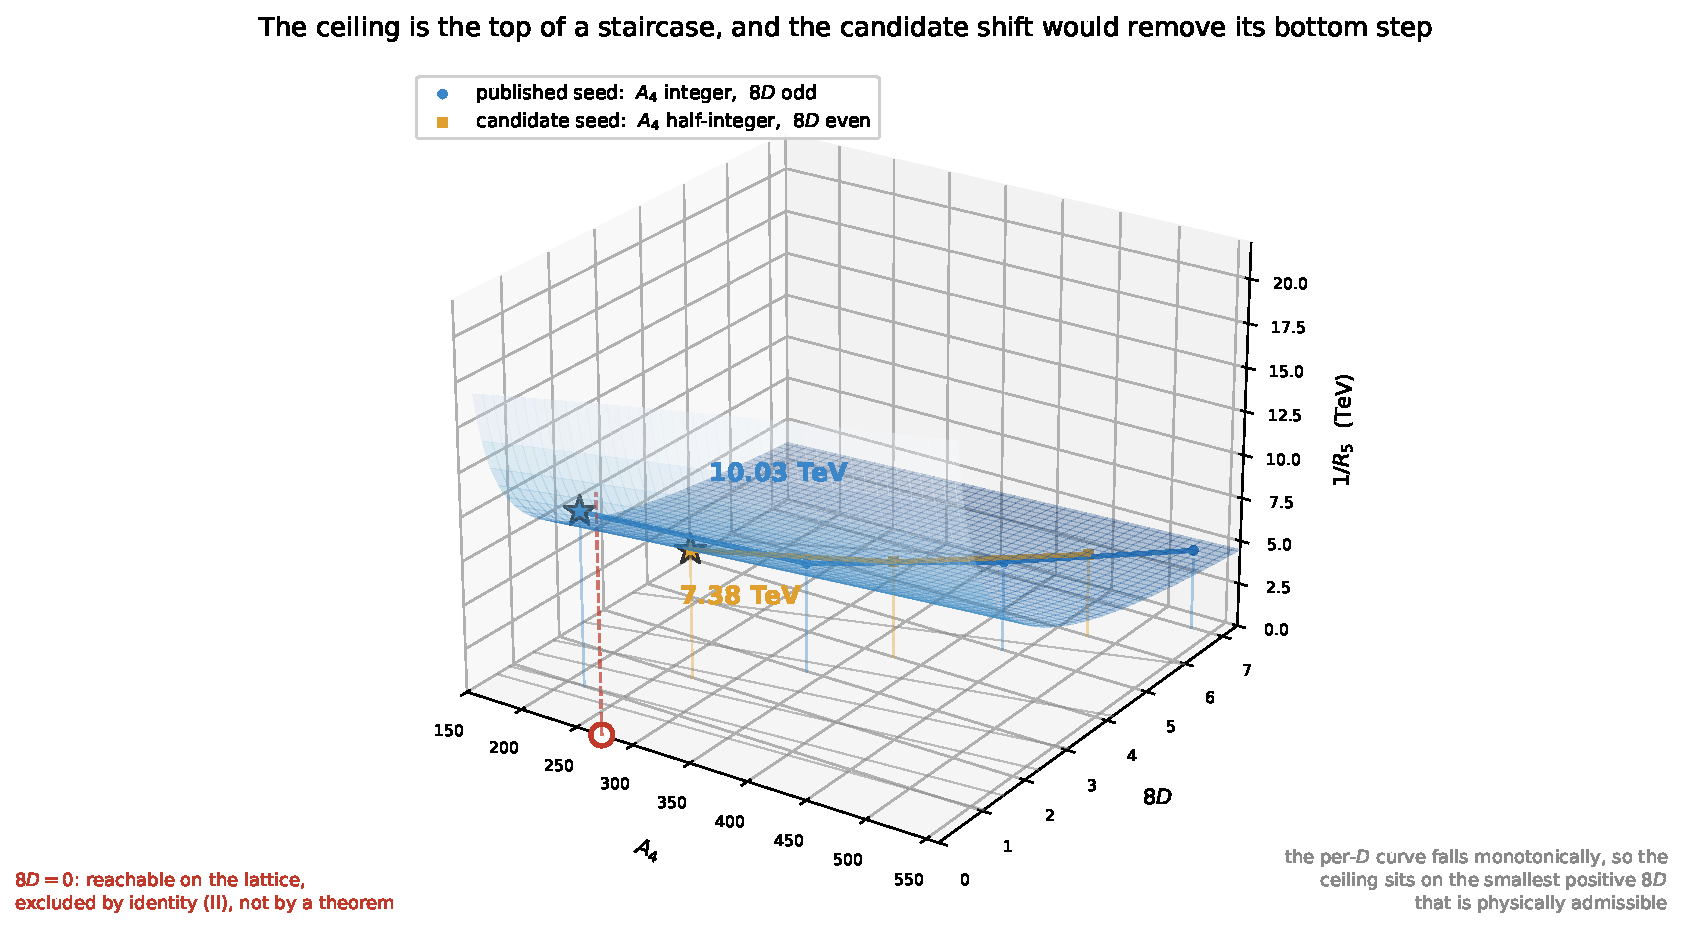
\includegraphics[width=0.92\textwidth]{fig_coset3d.pdf}
\caption{\textbf{The ceiling is the top of a staircase, and the candidate shift would remove the bottom step.} Each marker is the certified upper bound on $1/R_5$ at that value of $8D$ --- the LP dual over the moment cone, not an attained optimum; the surface behind them is the objective $1/R_5=2\pi m_W/x$, which diverges as $8D\to0$. The two lattices interleave in the base plane: with \cite{KM25}'s coefficients $A_4$ is an integer and $8D$ is odd, so the staircase starts at $8D=1$ and the ceiling is $10.03$~TeV; on the \emph{candidate} parity-resolved seed $A_4$ would become half-integral and $8D$ even, the $8D=1$ step would no longer exist, and the ceiling would be $7.38$~TeV at $8D=2$. The bound is not lost on either branch; it is demoted by one step. The open circle at $8D=0$ is the honest part: the \emph{candidate} lattice does reach it, and what forbids it there is identity~(II), since $6\mu+A_4>0$ for every content forces $x=0$; on the published lattice $8D$ is odd and $8D=0$ is not on it at all. Both curves are computed by the same program, which reproduces the published $10.03$~TeV before it is allowed to report anything else.}\label{fig:coset3d}
\end{figure}

\textbf{What it costs is not the number but the reason.} With the odd-eighths theorem, $8D=0$ was
impossible and nothing had to be argued. Without it, $8D=0$ \emph{is} reachable on the lattice ---
nine copies of $\mathbf{28}(+,-)$ get there --- and what excludes it is that identity~(I) would
demand an infinite $G$, and --- more cleanly, and with no appeal to the optimisation --- that
identity~(II) settles it in one line. It reads $x^2(6\mu+A_4)=12\zeta(3)D$. Every bulk multiplet
contributes a \emph{non-negative} amount to $A_4$, which is the property the integer program
already relies on, and the gauge sector's own $A_4$ is $-\tfrac{27}{2}$ on the candidate seed;
meanwhile $m_h\in[125,127]$~GeV with $g_4=0.63$ puts $6\mu$ between $481$ and $496$. So
$6\mu+A_4>0$ for \emph{every} content, without exception and without a caveat. Then $D=0$ forces
$x=0$: there is no finite electroweak vacuum on this surface compatible with the measured Higgs
mass. That is a
physical argument about a limit, not a theorem about integers, and it is weaker. We would rather
say so than let a bound keep the standing it had when a theorem was holding it up.

\emph{So the honest way to present the whole of it is not as a doubt but as a fork, with both
branches costed.} The gauge seed enters everywhere through two numbers, the weights $(a,b)$ per
charged adjoint pair, and once they are named the rest is bookkeeping:

\begin{center}\footnotesize
\rowcolors{2}{white}{softgrey}
\begin{tabular}{lcc}
\toprule
\rowcolor{hdrblue!10} & seed printed in \cite{KM25} & candidate $(3{+}1)$ seed \\
\midrule
weights $(a,b)$ per charged pair   & $(2,\tfrac12)$        & $(\tfrac32,\tfrac12)$ \\
gauge bracket                      & $(2,4,7)$             & $(\tfrac32,3,6)$ \\
$8D$ from the gauge sector         & $-27$, \textbf{odd}   & $-18$, \textbf{even} \\
$A_4$ from the gauge sector        & $-18$, integer        & $-\tfrac{27}{2}$, half-integer \\
$2W$ from the gauge sector         & $-3$, odd             & $-3$, odd \\
$32F(0)/\zeta(5)$ from the gauge   & $9$, \textbf{odd}     & $18$, \textbf{even} \\
parity of the three rungs $k=0,1,2$& odd, odd, \textbf{even} & even, even, \textbf{odd} \\
is $A_4=0$ in the coset?           & yes, $A_4\in\ZZ$      & no, $A_4\in\ZZ+\tfrac12$ \\
\midrule
\rowcolor{amber!14}hypothesis of Thm~\ref{thm:eighths}& \textbf{satisfied}    & \textbf{not satisfied} \\
Thm~\ref{thm:mod6}, $8D\equiv2A_4+3$ & holds               & holds \\
$2W$ odd for every content         & holds                 & holds \\
\rowcolor{amber!14}$|F(0)|\ge\zeta(5)/32$             & holds                 & \textbf{not proved} \\
Lambert closed form, ladder, kernel& holds                 & holds \\
\midrule
smallest positive $D$ the ceiling can sit on & $\tfrac18$  & $\tfrac28$ \\
what forbids $D=0$                 & a theorem             & identity~(II) \\
LP-dual ceiling on $1/R_5$         & $10.03$~TeV           & $7.38$~TeV \\
attained optimum; true vacuum      & $10.01$; $9.22$~TeV   & not recomputed \\
\bottomrule
\end{tabular}
\end{center}

\noindent \textbf{Read down the second block and the shape of the result is visible at once.} Some
of the load-bearing statements are indifferent to which column is right and some are not, and the
table is the only place that says which is which. Two rows deserve a second look. The value bound
$|F(0)|\ge\zeta(5)/32$ is not merely rescaled on the candidate branch: its \emph{proof} goes, since
$32F(0)/\zeta(5)$ reads $9$ on one seed and $18$ on the other, and an even integer is not kept away
from zero by being an integer. And $A_4=0$, which the published branch reaches and rules out on
physical grounds, is not even in the candidate coset --- there $A_4$ is half-odd-integral, so the
obstruction stops being a physical argument and becomes arithmetic. \emph{Quantised does not mean
non-zero; \textbf{oddly} quantised does}, and separating those two took a second seed to see.

\noindent \textbf{And the table is easier to read once the right object is named.} It is not the
half-integer, and it is not the three colours: both of those are properties of one seed that happen
to be true. What the whole table turns on is the \emph{parity character of the affine gauge base
point}. On the row that mixes the two sectors,
\begin{keyeq}
\begin{equation}\label{eq:chigauge}
  \begin{aligned}
    \chi_{\mathrm{gauge}}(a,b)\;&\equiv\;(2a)+(2b)\ \ (\mathrm{mod}\ 2)\,,\\[2pt]
    \chi_{\mathrm{gauge}}\bigl(2,\tfrac12\bigr)=1\,,\qquad
    &\chi_{\mathrm{gauge}}\bigl(\tfrac32,\tfrac12\bigr)=0\,.
  \end{aligned}
\end{equation}
\end{keyeq}
\noindent Read the table again with that in hand and every row explains itself. The mod-six law
survives because it lives in $8D-2A_4$, whose residue at the base point is $9$ on \emph{both} seeds
--- it never sees $\chi_{\mathrm{gauge}}$ at all. The oddness of $2W$ survives because $2W$ lives in
the \emph{difference} of the two charge-one weights, where a common shift cancels. The oddness of
$8D$ does not survive, and neither does the gap below $|F(0)|$, because both read
$\chi_{\mathrm{gauge}}$ directly. \emph{One character, four rows, and no coincidences left over.}

\noindent \textbf{And once the object is named, the whole table is one contraction.} Two seeds are
two base points of the same affine lattice, so what separates them is a \emph{vector}. In the
integer coordinates $(2A_4,8D,2U,V,2W)$ it is
\[
  \Delta_{\mathrm{seed}}\;=\;(9,\;9,\;9,\;0,\;0),
\]
derived from the three numbers of the gauge bracket and nothing else. A statement written as a
linear functional $\ell$ on the content then survives the change of seed exactly when
$\ell(\Delta_{\mathrm{seed}})$ vanishes in the modulus that statement is written in --- and every
row above is that one contraction. $8D$, $2A_4$, $2U$ and $32F(0)/\zeta(5)$ each pick up $9$, which
is odd, so all four flip. $2W$ picks up $0$, because it reads the \emph{difference} of the two
charge-one weights and the candidate moves both by the same $\tfrac12$. And $8D-2A_4$ picks up
$9-9=0$ --- not zero \emph{modulo six} but zero, which is why Theorem~\ref{thm:mod6} survives for a
stronger reason than the rest. The same contraction settles, with no further proof, that the
$\bmod\,8$ congruence $8D\equiv2U$ of \eqref{eq:congr5} survives too. \textbf{So what a second seed
buys is not a second column: it is the vector between them}, and with it the list of which
observables are blind to a shift of the gauge base point and which detect it. Computed in
\texttt{seed\_\allowbreak shift\_\allowbreak character.py}, which derives the five gauge
coordinates from the bracket and only then compares them against the table, and which carries a
control that can fail: a fictitious seed moving the antiperiodic weight as well breaks the
invariance of $2W$, as it must. Figure~\ref{fig:seedshift} is the same statement drawn. Read down the third block and the bound does
not vanish on either branch --- it changes the coset that carries it, and with it the rung and the
number. \emph{That is a more interesting result than the one we set out to report, and it is only
visible because there are two columns.} A single-column paper cannot tell you which of its theorems
were resting on an inherited number.

\begin{figure}[t]\centering
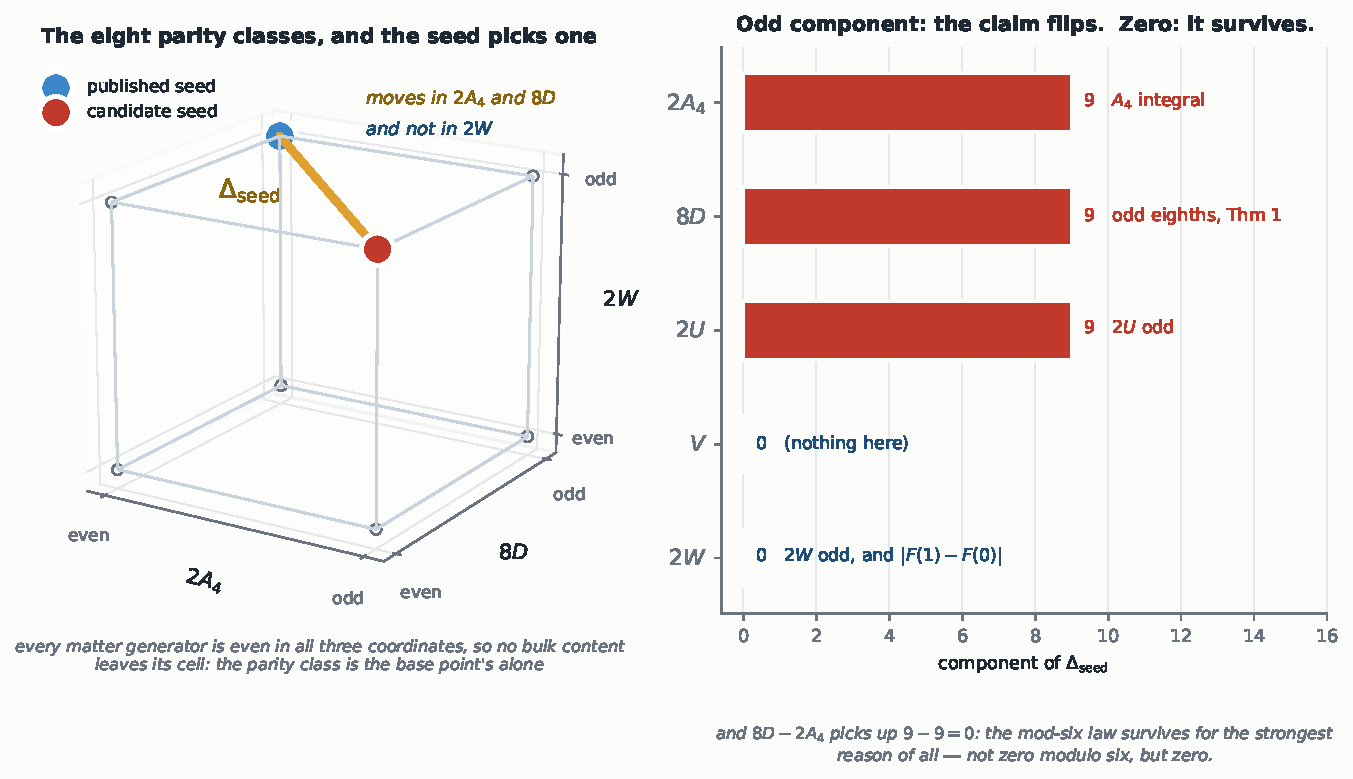
\includegraphics[width=\textwidth]{fig_seedshift.pdf}
\caption{\textbf{Two seeds, two base points, one vector.} \emph{Left:} the parity classes of
$(2A_4,8D,2W)$ are the eight vertices of a cube, and no bulk content can leave the one its seed
picks --- every matter generator is even in all three coordinates, so the class belongs to the
gauge base point and to nothing else. The seed \cite{KM25} print sits at
(even,\,odd,\,odd); the candidate of \S\ref{sec:open} at (odd,\,even,\,odd). The amber segment
is $\Delta_{\mathrm{seed}}$ read modulo two: it moves $2A_4$ and $8D$ and leaves $2W$ where it
was, which is the whole of why the hypothesis of Theorem~\ref{thm:eighths} fails on the candidate
branch while the $2W$ theorem does not even notice. It is a face diagonal and not an edge,
because two coordinates change and one does not. \emph{Right:} the five components of
$\Delta_{\mathrm{seed}}$ and the statement that lives in each --- an odd component flips its
claim, a zero leaves it standing. Drawn by \texttt{make\_\allowbreak fig\_\allowbreak
seedshift.py}, which takes the eight generators from \texttt{congruences.py} rather than
retyping them, and refuses to draw unless all eight are even in those three coordinates and a
fictitious seed that also moves the antiperiodic weight lands on a different
vertex.}\label{fig:seedshift}
\end{figure}
\noindent \emph{Every route in Parts~I--VII enters the causal chain at the coefficient end and
runs backwards.} What would close it is not another consistency check but a calculation in the
other direction: a Coleman--Weinberg sum over the six-dimensional Kaluza--Klein tower with these
orbifold parities, returning the weight of a $P_6=-1$ pair from its antiperiodic moding rather
than reading it off. \textbf{And that calculation appears not to exist in published form}, which
turns a private weakness into something worth doing on its own account. \cite{HY04} give the general one-loop
Wilson-line potential for five-dimensional $\su{N}$ on $S^1/\ZZ_2$, valid for arbitrary
representations and boundary conditions --- it is what \S\ref{sec:anchor} runs. We could find no
six-dimensional counterpart: the recent $T^2/\ZZ_4$ study of \cite{TZ4} writes model-specific
potentials rather than a general formula and does not treat $T^2/\ZZ_2$ with two independent
parities at all. So the missing object is the six-dimensional analogue of \cite{HY04}, and deriving
it would both close the one inferred link in this paper's chain and supply a formula the field does
not have. Until then the strongest statement in \S\ref{sec:collider} --- \eqref{eq:combchi}, which
reads the comb and therefore the seed, and not \eqref{eq:tulimit}, which does not --- has one
determination and no
second opinion.
\item \textbf{The antiperiodic sector is unanchored, and that is not an accident.} Every published
check a curvature can be anchored against sits at $B=0$, and on that locus $\Delta_k=\mathcal{A}_k=S_k$: the parity-weighted moment and
the parity-blind one are the \emph{same function} there. So no published check can separate $A$
from $B$, and in particular none of them tests the $-\tfrac34$ of $D=A_2-\tfrac34B_2$ --- the one
coefficient every theory-side scale in this paper passes through. That is the blindness, and it is
structural rather than a gap in the reading: each of the three things the surrounding
literature does with a parity stays on the locus. \cite{vGIQ} build the
twisted trace itself --- their (4.42)--(4.43) carry $\mathrm{Tr}(\lambda_R T^{A'}_R T^A_R)$, the parity
inserted in the trace, as the candidate brane term --- and then prove it \emph{vanishes} on
$S^1/\ZZ_2$, their abstract concluding that all brane effects for the Higgs mass do. \cite{CCD24}
split the sum by parity, but at $p=5$ and comparing values at two orbifold points; the words
\emph{curvature}, \emph{second derivative}, \emph{Dynkin} and \emph{trace} do not occur in their
forty-five pages. (That comparison at two points is not idle for us --- \eqref{eq:truevac} is it,
and it is what removes eight hundred GeV from the ceiling. It is blind to the split all the same:
it reads the \emph{value} of the potential, which is the $p=5$ rung, and the anchor question is
about the $p=3$ one.) And \cite{PGY24}, studying the same Wilson-line potential non-perturbatively on
$\mathbb{R}^4\times S^1$, records that increasing the number of fermions is equivalent to adding a parity
pair --- which is exactly true where they say it and exactly false here, and the two moments say
why in one line: on our lattice a parity pair has $\Delta=0$ for every one of the four multiplets
but $B\neq0$ for all four, so a pair moves along the \emph{unanchored} axis while leaving the
parity-weighted moment untouched, and a multiplicity does the reverse. Identifying them is
identifying a direction the literature measures with one it does not.
\textbf{Nobody has had a reason to leave the corner, because
inside it the three operations coincide.} That is why an anchor for $B\neq0$ has to be
computed rather than found, and it is the sharpest thing this paper is missing.

Two measurements say how sharp, and they are in \texttt{anchor\_\allowbreak delta.py}. First, the
residual is \emph{not} a function of the parity-blind moments: rows (1) and (2) of \cite{KM25}'s
table have identical $S_0,S_1,S_2$ to the last digit --- $87.5$, $179.5$, $707.5$ --- and their
residuals differ by twenty-five per cent, which no ordering over five collinear points could have
established. Second, the split is a near-cancellation: $D=A_2-\tfrac34B_2$ is $78.000-76.125$ on
row (1), a $2.4\%$ residue, and the leverage that gives is measured rather than estimated: rows (1)
and (2) differ by one per cent in the split, $78.000-76.125$ against $79.000-75.375$, and their $D$
differ by a factor of $1.93$ --- so $\alpha_{\min}\sim\sqrt D$ moves by $39\%$, the size of the
residual itself. Rescaling the
antiperiodic sector by a single $\lambda$ does not repair the five rows, and it is $\lambda-1$ that
has to be judged: the required perturbation runs from $0.2\%$ to $1.4\%$, a factor of seven, so
this joins the one-parameter repairs already excluded in Part~VI. But it is of one sign and of
\emph{that} order on every row, which changes what the caveat asserts. It is not that the potential
is wrong by a factor of two; it is that one trace may be wrong in its second digit, in the one
place where $D$ has no room.
\item \textbf{The other two congruences are read, and one of them is already in this paper twice.}
\eqref{eq:snf5} gives $\ZZ^5/L\cong\ZZ_2\times\ZZ_{72}\times\ZZ_{2592}$. As Smith prints them the
last two are unreadable --- five-digit coefficients modulo $72$ and $2592$ --- but $72=8\cdot9$ and
$2592=32\cdot81$ are coprime factorisations, so each is really \emph{two}. In lowest terms, and
\emph{on the affine coset based at the gauge seed \cite{KM25} print} --- the residues below are the
coset's, not the matter sublattice's, which has residue zero in every one of them --- every bulk
content satisfies
\begin{equation}\label{eq:congr5}
\begin{aligned}
  8D+2U+2W&\equiv1 &&(\bmod\ 2), &  8D&\equiv 2U+4(2W) &&(\bmod\ 8),\\
  A_4+8D+3(2U)&\equiv V &&(\bmod\ 9), &
  2W&\equiv-\bigl(2A_4+12(8D)+3(2U)\bigr) &&(\bmod\ 32),
\end{aligned}
\end{equation}
together with $V\equiv0\ (\bmod\ 81)$, which is automatic because $V$ is $81$ times a multiplicity.
The five moduli multiply to $2\cdot8\cdot9\cdot32\cdot81=373248$, the index, so this is the
\emph{complete} congruence description of the coset and not a sample of it. Checked in
\texttt{congruences.py} on the eight generators, the gauge sector, the witness of
Figure~\ref{fig:vacuum} and \cite{KM25}'s five rows, and against Smith's own form on a sweep of
$114\,244$ vectors, so that the readable statements are the same \emph{set} and not a weakening.

Two things come out. \textbf{The parity character is not one of the factors}: it is the joint
mod-two shadow of three of them, since the $\bmod\,8$ statement gives $8D\equiv2U$, the $\bmod\,32$
one gives $2U\equiv2W$, and the $\bmod\,2$ one then forces all three odd. So the oddness of $2U$,
which the previous edition of this list recorded as a gap, is \emph{equivalent} to the oddness of
$2W$ --- by a congruence that never mentions the $-\tfrac72$. And \textbf{the $\bmod\,9$ statement
is this paper's own divisibility}: reduced modulo three it reads $A_4+8D\equiv0$, which is at once
the step-three filter \S\ref{sec:ceiling} searches by and the remark in \S\ref{sec:arith} that
\cite{KM25}'s rows give $8D+A_4=273,300,198,234,270$, all divisible by three. Those are one fact,
and carrying $2U$ buys a further power of three.

What they do \emph{not} do is move the ceiling, and that is structural rather than a matter of
checking cases: the projection of the content lattice to the $(A_4,8D)$ plane has index exactly six
--- the gcd of its $2\times2$ minors --- so the mod-six rule is already the complete statement
there, and nothing involving $2U$, $V$ or $2W$ can cut the plane further. Whatever these forbid,
they forbid inside a fibre. The one escape would be a vertex whose fibre they empty, and the three
this paper argues about, $A_4=104,212,215$ on $8D=1$, each merely pin $2U$ to one class modulo
three, which the eight multiplets realise. What an odd $2U$ \emph{means} is therefore still open,
but it is no longer a separate gap from the $2W$ theorem.

\emph{And the four-coordinate projection comes with it.} The previous edition of the honest-limits
table recorded that the conditions behind $\ZZ^4/L\cong\ZZ_{18}\times\ZZ_{648}$ of \eqref{eq:snf}
were computed but not written out; eliminating $2W$ from \eqref{eq:congr5} writes them. \textbf{And the two levels must not be run together here of all places.} The projected
\emph{matter} lattice is the kernel of the four congruence maps --- $8D\equiv0\ (\bmod\ 2)$,
$8D-2U\equiv0\ (\bmod\ 8)$, $A_4+8D+3(2U)-V\equiv0\
(\bmod\ 9)$ and $V\equiv0\ (\bmod\ 81)$ --- with residue \emph{zero} in every one of them, as a
subgroup must have. Adding the gauge base point \cite{KM25} print translates that subgroup to the
affine coset, and it is \emph{there} that a content reads $1,4,0,0$. The two
readings genuinely differ in the second, where $4(2W)$ survives only because $2W$ is odd. Index
$2\cdot8\cdot9\cdot81=11664=18\cdot648$, confirmed by closing the subgroup of $(\ZZ/32)^4$ and
$(\ZZ/81)^4$ by brute force rather than by trusting the elimination. Two further questions survive.
Is the lifted
semigroup \emph{normal}? In the projection it is: no point of the cone-and-lattice is unreachable,
measured to $A_4=420$; if the lift has holes they are contents every visible law permits and no
bulk can build. And what is the vector partition function $N(A_4,8D,2U,V)$, which should be
quasi-polynomial on the chambers of the cone and would turn the degeneracies of
Figure~\ref{fig:collapse} from a measurement into a formula.
\item \textbf{Where does the third minimum bind?} The previous edition of this list asked whether
$W>0$ is sufficient as well as necessary, and proposed the semi-infinite programme as the way to
find out. \S\ref{sec:ceiling} now runs it, and the answer has two halves. On the rung that decides
the ceiling the programme generates exactly one cut, the one at $y=1$, so there $W>0$ is the whole
of the true-vacuum condition and \eqref{eq:ceilingtrue} needs no screen. But a content invisible to
both symmetric points does exist --- \eqref{eq:semiinf} demands a second cut on $8D=3$, and
\S\ref{sec:ceiling} places it at the exact rational holonomy $y=2/3$, where the depth is the
closed-form functional $-\tfrac{121}{81}\zeta(5)[C_1+C_2+C_4]$ --- so the phenomenon is real, it is
exact, and it merely fails to reach the deciding rung. What is now open is smaller and sharper: is
there a rung on which a cut other than $y=1$ moves the \emph{ceiling} rather than an interior
vertex? And where the \emph{other} cuts sit is now a measured negative rather than an untried
question: across $6560$ contents the $2956$ interior minimisers stand only $1.05$ times closer to
the rational skeleton $\{1/3,1/2,2/3\}$ than chance does. The $y$ at which a given content's third
minimum sits still ought to be readable off its charges the way $\amin$ is, and is not --- and the
nearest rational holonomy is now known not to be the way to read it.
\item \textbf{A remainder bound uniform in the rung.} \eqref{eq:rigorousceiling} is proved over the
first seventy odd rungs and not past them, and the reason is measurable: the bound's relative bite
$\delta/\hat x$ climbs from $2.5\times10^{-4}$ at $8D=1$ to $9.0\times10^{-1}$ at $8D=1201$, so it
loosens faster than the truncated ceiling falls and eventually certifies nothing. That is a defect
of the \emph{bound}, not of the ceiling --- \eqref{eq:slope} proves $M(k)\le6268$~GeV on every rung $k\ge3$
with no scan at all. What is missing is a bound on $|R'_j(\hat x(k))|$ decaying at least as fast as
the curvature $\propto k$, which would close \eqref{eq:rigorousceiling} for all $k$ in one line. The
per-multiplet remainders are explicit Li$_5$ tails, so this looks like an exercise in bounding
$\sum_{n>N}\sin(nc\hat x)/n^4$ uniformly in $\hat x\to\hat x_\infty$ rather than an open problem;
we have not done it.
\item \textbf{The $215$-versus-$212$ margin is smaller than the expansion that produced it.} One
part in $10^{4}$, against a closed form good to $0.13$--$0.62\,\%$. The remedy is not more digits
but the corrected identities: redoing the elimination \emph{without} discarding the remainder
$R$ gives $x^2(6\mu+A_4)=12\zeta(3)D-18R'/x+6R''$ and a matching correction to (I), and
\S\ref{sec:closed} has just established that $R$ is a convergent tail with a rigorous bound. Running
the integer program over certified intervals for $x$ rather than over the truncated surface would
turn $10.01$~TeV from a statement about the algebraic surface into one about the polylogarithmic
potential. That is the single most valuable thing left in this paper.
\item \textbf{What would turn the recast sensitivity into an exclusion. One thing now, and the
public-data programme is exhausted.} Three closures have been run and none of them is the missing
step. \emph{The observed limits}: aimed at \cite{CMSangular}'s published colour-singlet limit on
their own selection, the machinery returns $17.5$ against $17$~TeV and $29.5$ against $37$.
\emph{The expected ones}: an Asimov Standard-Model dataset through our own $\chi^2$ returns $1.08$
and $0.85$ against \cite{CMSangular}'s expected $18^{+20}_{-2}$ and $34^{+8}_{-5}$~TeV, close
enough to the observed $1.03$ and $0.80$ that the gap is the method and not this dataset.
\emph{And the template}, which was the sharpest of the three worries: the closure benchmark ought
to be the vector-like $VV$
operator and not only $LL$: the tower is $(\bar q\gamma^\mu T^aq)^2$, which sees both chiralities,
while the $17$ and $37$~TeV are left-handed, and the published $VV$ limits behave differently
enough --- the constructive one reaching some $50$~TeV, the destructive one developing
disconnected regions where the interference cancels against $1/\Lambda^4$ --- that agreeing with
one says little about the other. The machinery for it is in place --- \cite{CIJET}'s operator basis
is the chiral one of its eq.~(2), so $VV$ is $\lambda_1=\lambda_3=\lambda_5$ where the $LL$ closure
is $\lambda_1$ alone. \textbf{That run has now been done, and it settles the worry rather than
confirming it.} Paired selection against selection, on the constructive side where
\cite{CMSangular} publish a limit for both operators, the closure ratio moves from $0.80$ to
$0.78$ on their own contact-interaction selection, and from $0.69$ to $0.66$ over all seven mass
bins. Two selections, the same direction, and \textbf{two to three points either time}. \emph{So
the chirality of the template is not what the closure deficit is made of} --- which is worth
knowing, because it was the most plausible explanation available and it is now the least. What the
pairing does \emph{not} do is give the deficit a single size: it is $0.78$ on the matched
contact-interaction selection and $0.66$ over all seven bins, so the discrepancy is
selection-dependent and only the $LL$-to-$VV$ step is stable. On the destructive side
there is nothing to pair: \cite{CMSangular} publish no $VV$ limit there. And the deficit stays what
it was, \textbf{closure accuracy and not a transferable multiplicative systematic}; measuring it
twice does not turn it into a band. \textbf{What remains is one step, and it is the one that costs
something}: the limit should be set the way \cite{CMSangular} set theirs,
with detector-level Poisson likelihoods, profiled nuisances and $CL_s$. Until then
\eqref{eq:tulimit} is a sensitivity and is written as one. \textbf{And a second systematic sits
beside it, of a different kind and unmeasured}: the baseline is \cite{CMSangular}'s
next-to-next-to-leading-order QCD while the tower's deformation is validated against
\cite{CIJET} at leading order, so the two enter \eqref{eq:chisq} at different orders. The
$0.2\,\%$ closure is an implementation check of the leading-order interference and not a
statement about the missing $K$-factor; how far an NLO deformation would move
\eqref{eq:tulimit} is not measured here, and it is the cheapest of the open collider
questions to answer.

\item \textbf{The thermal holonomy literature has not been swept.} \S\ref{sec:parity} makes the two
problems one family; that literature has $V''(0)\propto T(R)$ as textbook and $\ZZ_2$-projected
traces as natural bookkeeping, so it is the highest-prior remaining place the bridge could already
exist. It is named here as an open gate, not as a null.
\item \textbf{Two loops.} The map computed here is a one-loop map. At two loops the potential sees
more of the content --- a weight $W(w,w')=\sum_a|\langle w|T^a_R|w'\rangle|^2$ rather than a
multiplicity --- and what that second rung is blind to is decidable without a loop integral.
\item \textbf{Gauge coupling unification, which is their own open question.} \cite{KM25} close by
asking for it: $\su3_C$ and $\su4$ sit inside one $\su7$, so the couplings must meet where the
symmetry is restored, and they leave the one-loop analysis to future work. Half of it is settled
here and costs nothing: below $1/R_5$ the theory is the Standard Model, so
$\alpha_2^{-1}-\alpha_3^{-1}$ is $19.2$ at $2$~TeV and $18.2$ at the certified ceiling --- it barely
moves across the whole allowed range, because four-dimensional running has under five e-folds to
work with and closes the gap at $0.61$ per e-fold. \textbf{The entire burden therefore falls on the
Kaluza-Klein tower}, and the ceiling of \S\ref{sec:ceiling} is not a bystander: it fixes where that
tower may begin. The other half --- whether the $\su7$ tower, whose levels the orbifold projection
leaves incomplete, can close $18.2$ before perturbativity ends --- is a computation, not an opinion,
and it is the natural next paper.
\item \textbf{Does the theorem's dimension have a general statement?} \S\ref{sec:arith} shows the
protection is absent from the five-dimensional class \cite{HY04}'s formula covers --- $\su{N}$ on
$S^1/\ZZ_2$ with a single Wilson phase, where every rung is even and $D=0$ is reached by three
multiplets --- while here the rungs below the fourth moment are odd. The mechanism is the parity
character \eqref{eq:chigauge} of the gauge base point --- not a single half-integer --- and a
second independent parity is what supplies the extra affine character that
\emph{can} make a rung odd --- in this construction, which is as far as one model reaches.
Whether
\emph{odd rung $\Leftrightarrow$ second parity} is a theorem --- across $T^2/\ZZ_N$, and in seven
dimensions --- is not settled by one model.
\item \textbf{Does the periodic/antiperiodic split organise the counterterms?} It does at the pole:
\eqref{eq:ladderab} sends the antiperiodic half to zero at $p=1$, so the branch point is fed by the
periodic moment alone. Whether that coincides with the bulk-localised divergent structure, with the
complementary parity sector feeding the boundary terms, is an interpretation and not a consequence
of the rung: it needs an explicit counterterm calculation. Whether the same
split works away from the pole --- one half feeding the higher-derivative bulk operator, the other
the boundary-localised one --- is what the Hurwitz correspondence of \S\ref{sec:novel} opens and
does not answer.
\item \textbf{The lattice, counted.} The multiplet lattice with its congruence is a rational cone
intersected with an affine sublattice, so the number of contents at fixed $(A_4,8D)$ is a vector
partition function, and Theorem~\ref{thm:mod6} supplies one residue-class constraint underlying its
chamberwise quasi-polynomial structure. \emph{Not} that six is the minimal quasi-period: nothing
here shows that, and a congruence on the lattice is a weaker statement than a period. That is
machinery this paper
uses only in its polyhedral half.
\end{itemize}

% ===================================================================
\section*{The ledger}
\addcontentsline{toc}{section}{The ledger}

% \footnotesize here, \scriptsize in the Spanish edition -- one notch, in this one block, and the
% only difference in setting between the two.  That edition carries about 4 % more rendered text
% because Spanish runs longer, so at equal settings it came out a page longer; see the note at
% its own ledger for why a symmetric adjustment cannot fix that and why the difference is
% absorbed here rather than in the prose.  Re-check both page counts before changing either.
\begingroup\footnotesize
\begin{longtable}{p{0.62\textwidth}p{0.31\textwidth}}
\toprule
\rowcolor{okgreen!12}\textbf{Established, and how} & \textbf{Where}\\
\midrule
\endfirsthead
% The ledger changes verdict as it runs -- established, corrected, withdrawn, open -- so repeating
% the green "Established" header on the continuation pages would put that word above rows that are
% withdrawn or open. It did, until this was fixed. The continuation header is neutral.
\toprule
\textbf{The ledger, continued} & \textbf{Where}\\
\midrule
\endhead
$\amin$ in closed form: median $0.13\,\%$ over $272$ contents, $0.209\,\%$ over the five published
rows, against our own numerical minimisation of the same potential &
\S\ref{sec:closed}; the no-logarithm control fails by $+104$ to $+174\,\%$\\
$F''(\amin)=\pi^2[2\zeta(3)D-A_4x^2/6]$: the logarithm and $G$ cancel at the stationary point, so
both columns of their Table~1 follow from $(D,A_4)$ with no minimisation --- \emph{our}
reconstruction of the two, not their published $\amin$ &
\S\ref{sec:mh}\\
The two logarithm-free identities, verified to $6\times10^{-14}$ &
\S\ref{sec:ceiling}, eq.~\eqref{eq:two}\\
$8D$ is an odd integer, so $D\ne0$ and \emph{the symmetric point} is never marginal ---
\textbf{conditional on \cite{KM25}'s gauge seed}; the matter half of the argument is not &
\S\ref{sec:arith}, \S\ref{sec:open}; $4096$ parity assignments, no counterexample\\
$8D\equiv2A_4+3\pmod6$, from $c^4\equiv c^2\pmod3$ --- \textbf{holds on either gauge seed} &
\S\ref{sec:arith}; the five published rows and all eight generators\\
$|F(0)|\ge\zeta(5)/32$, the bound attained --- \textbf{conditional on \cite{KM25}'s gauge seed}:
it reads \eqref{eq:chigauge} exactly as the odd eighths do, and on the candidate seed
$32F(0)/\zeta(5)$ is even & \S\ref{sec:arith}, \S\ref{sec:open}\\
The ladder is geometric with ratio $c^2/4$, charge two its fixed point; and
$O(5)-O(3)=4[O(3)-O(1)]$ whenever no third mode opens & \S\ref{sec:ladder}; $4096$ assignments,
and a prediction confirmed on all eight multiplets\\
The ladder continues past its own pole to $p=-1,-3,\dots$, where $\zeta$ is rational: exactly one
logarithm exists, at order $x^4$, and the remainder is a convergent tail for $|\alpha|<1/c_{\max}$ &
\S\ref{sec:closed}; term ratios $(c\alpha)^2$ and $(c\alpha/2)^2$, with controls past both radii\\
$A_4=0$ forces $8D\equiv3\pmod6$, so the analytic branch cannot reach the quantum $8D=1$; and on
that branch no content has both $D>0$ and $W>0$ --- \textbf{stated on the seed \cite{KM25}
print}, the candidate coset having $A_4\in\ZZ+\tfrac12$, where $A_4=0$ does not occur at all &
\S\ref{sec:arith},
eq.~\eqref{eq:analytic}; eleven base solutions, one free multiplet, exact arithmetic, and it misses
by one step\\
$2W$ is an odd integer, so $|F(1)-F(0)|\ge\tfrac{31}{32}\zeta(5)$: in \emph{this} model the two
symmetric points are never degenerate, hence never equivalent descriptions of one orbifold ---
unlike \cite{CCD24}'s, where they are &
\S\ref{sec:ceiling}, eq.~\eqref{eq:nevermarginal}; \textbf{not} the same half-integer as
Theorem~\ref{thm:eighths}, which an earlier version of this row said it was: $2W$ reads the
\emph{difference} of the two charge-one weights, so it holds on \emph{either} gauge seed where
$8D$ odd does not. Checked on $3003$ contents\\
$M_{\mathrm{KK}}^2$ sits on an arithmetic comb of spacing $8\pi^2m_W^2/(\zeta(3)\,8D)$, necessary and
not sufficient & \S\ref{sec:pred}, eqs.~\eqref{eq:comb}--\eqref{eq:comb2}\\
The charge-two parity flip is the only log-free one, with signature $(-7,-16,-100/3)$ &
\S\ref{sec:ladder}, eq.~\eqref{eq:c2flip}\\
$1/R_5\le10.03$~TeV for arbitrary bulk content, by an exact rational dual --- \textbf{on the seed \cite{KM25} print} & \S\ref{sec:ceiling};
dominates all $1097$ window contents found to $N=14$\\
$G=\tfrac{25}{12}A_4-U\ln2-V\ln3$ lifts the content to a \emph{four}-dimensional lattice with
$\ZZ^4/L\cong\ZZ_{18}\times\ZZ_{648}$, where the relaxation's vertex $(215,1)$ is empty and the
bound sharpens to $10.01$~TeV \emph{attained} & \S\ref{sec:ceiling},
eqs.~\eqref{eq:snf}, \eqref{eq:ceilinginteger}; rank and invariant factors in
\texttt{lattice\_\allowbreak rank.py} and independently in Sage,
\texttt{lattice\_\allowbreak rank.sage}; the maximum over a finite feasible set at fifty digits,
the witness rebuilt through \texttt{moments()}\\
The remainder past three rungs is bounded, not estimated, and is itself \emph{linear} in the
multiplicities, so it rides inside the certificate's own dual: $1/R_5\le10.037$~TeV on the
untruncated potential over the first $70$ odd rungs, $0.025\,\%$ above the truncated certificate;
beyond them the remainder bound loosens and certifies nothing & \S\ref{sec:ceiling},
eqs.~\eqref{eq:remainder}, \eqref{eq:rigorousceiling}; $32$ contents $\times$ four $\alpha$, zero
violations, and the bound refuses at $u\ge1$\\
\cite{CCD24}'s stability criterion, summed over a content, is a fourth \emph{linear} functional, so
it fits inside the same integer program; imposing it gives $1/R_5\le9.22$~TeV on the three-rung
surface, attained, whose witness on the exact potential gives $9157$~GeV. \textbf{The criterion is
theirs; only its use here is new} & \S\ref{sec:ceiling},
eqs.~\eqref{eq:truevac}--\eqref{eq:ceilingtrue}; closed against exact to machine precision on six
contents. Untruncated it is not yet a single number and not an interval either: the witness gives
$9157$~GeV, the first $70$ odd rungs are capped at $10.037$~TeV, and a bound over \emph{all} rungs
is open --- \S\ref{sec:open}\\
Part~VI's escape costs $10/8$ of $D$ exactly, so affording it forces $8D\ge11$ and lowers the
ceiling to $3.97$~TeV --- the content with the largest hierarchy is the one that cannot pay &
\S\ref{sec:ceiling}, eq.~\eqref{eq:escapeceiling}; same dual, and $857$ of the $1097$ can pay\\
Our machinery reproduces \cite{vGIQ}'s criterion, its three critical flavour numbers, its $\su2$
minimum and the whole group-theory bracket of its curvature formula & \S\ref{sec:anchor}; residue
$2/\pi^2$ to eight digits, a pure convention\\
A nominal recast sensitivity of $1/R_5>10.86$~TeV from the spacelike form factor alone --- no
width, no $\mathrm{BR}(G_n\to jj)$ --- putting the $3.97$~TeV escape branch a factor of three
below it & \S\ref{sec:collider}, eq.~\eqref{eq:tulimit}; against \cite{CMSangular}'s
$77\times77$ covariance with the scale profiled, on a machinery that returns their own
contact-interaction limit as $17.5$ against $17$ and $29.5$ against $37$~TeV, and their
\emph{expected} one as $1.08$ and $0.85$ --- so the gap to their $CL_s$ is the method and not a
fluctuation of these data. Putting the $s$ channel back, with the total width profiled and its
worst case at $\Gamma_{\mathrm{exotic}}=0$, costs $1.03\,\%$\\
Read at the teeth of the per-rung ceiling comb rather than at an arbitrary mass, the recast says the
allowed region is not partly disfavoured but wholly so: the highest per-rung ceiling any bulk
content can reach on the seed \cite{KM25} print, $10.03$~TeV at $8D=1$, sits at $\Delta\chi^2=12.0$ against a threshold of
$3.84$, and the next tooth at $\Delta\chi^2=244$ & \S\ref{sec:collider}, eq.~\eqref{eq:combchi},
Fig.~\ref{fig:chi2}; nominal, from the same Gaussian recast, and stated as such\\
\midrule
\rowcolor{hdrblue!10}\textbf{Corrected here, and left visible} & \textbf{Why}\\
\midrule
``$1/R_5\le2.18$~TeV with the Higgs window'' & that is a bound on the \emph{size} of the content
($\le6$ multiplets), not on the model. Eight multiplets reach $9.14$~TeV. \S\ref{sec:ceiling}\\
``at moment zero marginality is reachable'' & true with pure component counts, false here --- but
not for the reason this row used to give. What forbids it is the parity character
\eqref{eq:chigauge} of the gauge base point, not a single half-integer and not the sixth dimension
on its own: the candidate seed is equally six-dimensional and has $\chi_{\mathrm{gauge}}=0$.
\S\ref{sec:arith}, \S\ref{sec:open}\\
Part~VI \S7's $1.94$ and $1.20$ quoted as a range & they are group means ($n=2$ and $n=3$); the
row-wise range is $1.03$--$2.08$, and \S\ref{sec:pred} uses the range\\
``the ceiling is attained at $(A_4,8D)=(215,1)$'' & the dual \emph{certifies} it there and the
lattice \emph{reaches} it, but no content of any size can pay for it in $G$ --- short by $0.067$ in
a budget of $681$. The vertex below can: $10.01$~TeV at $(212,1)$, attained, with a witness.
\S\ref{sec:ceiling}, eq.~\eqref{eq:ceilinginteger}\\
``sixteen contents with $A_4=0$'' & seventeen. The enumeration capped multiplicity at four per
multiplet while the sentence said six; the missing one has $D<0$, so the ``five with $D>0$'' stands.
\S\ref{sec:arith}\\
``the expansion is asymptotic'' & it is convergent for $|\alpha|<1/c_{\max}=1/3$, and every
$\alpha$ used here is inside that by a factor of at least $2.7$. \S\ref{sec:closed}\\
``$A_4=0\Rightarrow m_h\le29.6$~GeV, an exact margin'' & that number came from evaluating the
closed form at $\alpha\simeq0.89$, a factor $2.7$ \emph{outside} its own radius. Withdrawn and
replaced by \eqref{eq:analytic}, which uses no expansion at all. \S\ref{sec:arith}\\
``the $9.16$ of the enumeration against the $10.03$ of the certificate is the gap between a
relaxation and its lattice'' & it is not: it is the true-vacuum condition, which the enumeration
imposed silently through the global minimiser and the certificate did not impose at all. Named, it
becomes $9.22$~TeV attained. \S\ref{sec:ceiling}\\
``restoring the widths lowers the tower's contact coefficient by $2.55\%$, so $\Lambda_8$ is
low by $1.3\%$'' & there is no width to restore. In the spacelike channels every mode is below
its two-parton threshold, so the propagator is real; the giveaway is that the shift does not
switch off as $t\to0$. Withdrawn, and the tower summed exactly instead, \eqref{eq:resum}.
\S\ref{sec:collider}\\
``$3.97$~TeV is already inside the excluded region'' & the exclusions quoted are for a
\emph{narrow} resonance and this object has $\Gamma/M\simeq0.16$; the $s$-channel rate also needs
a branching ratio the model does not fix. Sensitivity, not exclusion --- and the angular recast,
now done, does not change that word: it is a Gaussian $\chi^2$ over unfolded data and not
\cite{CMSangular}'s detector-level $CL_s$. \S\ref{sec:pred}, \S\ref{sec:collider}\\
\midrule
\rowcolor{warmred!14}\textbf{Withdrawn, and left visible} & \textbf{Why}\\
\midrule
``the bracket of the gauge table is the number of colours, so the parity theorem and the death of
the obstruction are one product'' & true at their assignment, false on $3872$ of $4096$. A
coincidence at one point. \S\ref{sec:novel}\\
``the hierarchy is a quantised near-cancellation between bulk and brane'' & measured before it was
written: a $10\,\%$ effect, not $90\,\%$. What survives is a percentile statement about their five
rows. \S\ref{sec:novel}\\
``the parity-split mechanism is ours'' & it is published at $p=5$ \cite{CCD24}. Only the $p=3$ rung
and its consequences are claimed. \S\ref{sec:ladder}, \S\ref{sec:novel}\\
``the true-vacuum criterion of \S\ref{sec:ceiling} is ours'' & it is not: \cite{CCD24} \S2.2 states
it, proves its identities and draws its sign rule. Only its use inside the integer program is
claimed. \S\ref{sec:ceiling}, \S\ref{sec:novel}\\
\midrule
\rowcolor{amber!14}\textbf{Open, and stated as open} & \textbf{Why}\\
\midrule
Their Table~1 $\amin$ column is not reproduced by our assembly & Part~VI \S7; \S\ref{sec:anchor}
narrows the locus to the model dictionary but does not close it\\
The antiperiodic sector is unanchored & no independent published \emph{curvature} anchor tests
$B\neq0$; the parity-split results that exist stop at the value rung $p=5$. At $B=0$, $\Delta$ and
$S$ coincide. \S\ref{sec:anchor}\\
\cite{vGIQ}'s $\su3$ adjoint minimum $0.29$ against our exact $1/3$ & the centre control favours
ours; not proved, so not called an erratum. \S\ref{sec:anchor}\\
What an odd $2U$ \emph{means} physically & the congruence is now written,
\eqref{eq:congr5}, and ties $2U$ to $2W$; the interpretation is still missing. \S\ref{sec:open}\\
Is the lifted semigroup normal? & the projected one is, to $A_4=420$. \S\ref{sec:ceiling}\\
Where does the third minimum bind? & settled where the bound is decided: on $8D=1$ the
semi-infinite programme generates only the $y=1$ cut. On $8D=3$ it demands one, and that one is
exact at $y=2/3$, so the phenomenon is real and does not reach. Where the \emph{other} cuts sit is
a measured negative: the interior minimisers do not crowd the rational skeleton.
\S\ref{sec:ceiling}\\
The thermal holonomy literature is not swept & \S\ref{sec:parity} makes it the same family, so it
is the highest-prior place the bridge could exist. \S\ref{sec:open}\\
Is the recast sensitivity an exclusion? & $10.86$~TeV, and $13.75$ on their own contact-interaction
mass range, both clear $9.09$ and $10.03$. But a Gaussian $\chi^2$ over unfolded data is not
their detector-level $CL_s$, and the two closure benchmarks differ by interference physics rather
than by a calibration. Observed and expected closures diagnose a discrepancy of order ten to twenty
per cent in $\Lambda$ on the matched contact-interaction selection, and larger over all seven bins;
none of them defines a transferable uncertainty. Closing the likelihood is what would settle the
ceiling.
\S\ref{sec:collider}\\
Every theory-side scale carries the anchor residual & \S\ref{sec:setting}; the collider recast
does not, since it never passes through $\amin$. The ceiling is quoted with it in
\S\ref{sec:pred}\\
The anchor residual is a \emph{trend}, not scatter, and both ceilings sit outside the range that
measures it & sorted by $D$ the five ratios are monotone, $2$ of $120$ pairings, $p=0.017$; but
$A_4$ orders them equally well and five rows cannot separate the two moments. The ceiling is
certified at $D=1/8$ against an anchored $[1.125,3.625]$, the escape ceiling at $A_4=727$ against
$[189,271]$. \S\ref{sec:setting}, \S\ref{sec:pred}\\
\bottomrule
\end{longtable}
\endgroup

\section*{Data availability}

% Data availability va JUSTIFICADA, como el resto del articulo.  Llevaba
%   \begingroup\raggedright\sloppy\emergencystretch=4em
% sin comentario, y se veia: era la unica pagina con el margen derecho dentado.  Medido
% antes de tocarlo --- quitarlo no anyade ni un Overfull ni un Underfull al .log, y la
% pagina renderizada cabe mas texto por linea.  Los \texttt{} largos y la URL se rompen
% solos con el \allowbreak que ya llevan.  Si alguien lo repone, que sea con una medida
% detras y no por si acaso.
\begingroup
The paper in both languages, every script, every archived run and the figure sources are at
\href{https://github.com/karlesmarin/su7-compactification-bound}{\texttt{github.com/karlesmarin/su7-compactification-bound}},
which is where corrections to this paper will appear; the other six parts of the series have a
repository each, linked from that one.
Every displayed number in this paper regenerates from the ancillary scripts, whose standard output is
archived beside them in \texttt{outputs/}; the ledger above cites the script for each entry rather
than the number alone, so a reader who disagrees with a claim can re-run the thing that made it.
The principal artifacts are
\texttt{bernoulli\_\allowbreak clausen.py} (\S\ref{sec:parity}),
\texttt{ladder\_\allowbreak closed\_\allowbreak form.py}, \texttt{moment\_\allowbreak ladder.py},
\texttt{moment\_\allowbreak split.py} and \texttt{mechanism.py} (\S\ref{sec:ladder}),
\texttt{amin\_\allowbreak closed\_\allowbreak form.py} (\S\ref{sec:closed}),
\texttt{mh\_\allowbreak closed\_\allowbreak form.py} (\S\ref{sec:mh}),
\texttt{parity\_\allowbreak mod4.py} and \texttt{ladder\_\allowbreak obstruction.py} (\S\ref{sec:arith}),
\texttt{ceiling\_\allowbreak ilp.py} with its independent Sage lattice computation
\texttt{cone\_\allowbreak moments.sage}, the semi-infinite programme
\texttt{semi\_\allowbreak infinite.py} and the untruncated certificate
\texttt{rigorous\_\allowbreak ceiling.py} (\S\ref{sec:ceiling}),
\texttt{congruences.py} (\S\ref{sec:open}),
\texttt{prediction.py} and \texttt{hy\_\allowbreak predictions.py} (\S\ref{sec:pred}),
\texttt{vgiq\_\allowbreak anchor.py} with \texttt{vgiq\_\allowbreak charges.sage} (\S\ref{sec:anchor}),
\texttt{moduli\_\allowbreak space.py} (\S\ref{sec:novel}),
and \texttt{inverse\_\allowbreak map.py}, which reproduces Part~VI's \S7 by a route that shares no
arithmetic with it.
\texttt{formula\_\allowbreak map.py} states the formulas of Parts~VI and VII in minimal form and
checks the identities that link them, one to the next; the figures are drawn by
\texttt{make\_\allowbreak figures\_\allowbreak vii.py} from the same archive.
An interactive instrument, \texttt{tools/hierarchy\_\allowbreak explorer.html}, ships with the paper
and runs in a browser with no install and nothing leaving the machine: it computes the three rungs,
the closed form and the ceiling for a matter content the reader types in, so the claims of
\S\ref{sec:arith} and \S\ref{sec:ceiling} can be tried on a content this paper never saw.

\paragraph{And the collider layer, which needs three things that are not in this archive.} The
measurement is \cite{CMSangular}'s, on HEPData under \textsc{doi} 10.17182/hepdata.167852 and
released \textsc{cc0}; \texttt{fetch\_\allowbreak hepdata.py} fetches it, and the nineteen
tables travel with the ancillary files because that licence permits it. The parton densities are
CT10nlo \cite{CT10} through LHAPDF \cite{LHAPDF}, with NNPDF3.1 \cite{NNPDF31} and CT14nlo
\cite{CT14} for the set dependence of \eqref{eq:tulimit}; all three come from the LHAPDF set
repository at \texttt{lhapdfsets.web.cern.ch}, are freely available, and none is ours to ship.
\texttt{pdf\_\allowbreak provenance.py} reads each one's own \texttt{.info} and checks what has to
hold before it is used: the physical $(x,Q)$ our quadrature asks for lie inside the grid, the three
share $\alpha_s(m_Z)=0.118$, and --- because the product grid over mass and boost has corners with
$x>1$ that $x_1x_2=M^2/s$ forbids --- that all three return \emph{exactly zero} there rather than
extrapolating. They do; the unphysical corners carry no weight and the integral is the physical
one. That was never checked before a referee asked which set we used. And the contact-operator coefficients come from CIJET \cite{CIJET}, whose licence permits
academic use but forbids redistribution in any form: the program is therefore \emph{not} included
and neither is its output. What travels instead is the three input cards --- ours, and checked
against \cite{CMSangular}'s selection --- together with the command and the runtime needed to
regenerate the coefficient file, about nine hours on a desktop, written out in the archive's
\texttt{tools/cijet/README}. A reader who wants the collider numbers can obtain every ingredient
from its own source; what we may not do is hand any of them on.

\endgroup

\section*{Acknowledgements}

This paper stands on \cite{KM25}. Y.~Komori and N.~Maru wrote their model out fully enough that its
vacuum can be recomputed from their own equations rather than assumed, which is what Parts~VI and
VII both do, and they were explicit about where they had stopped. N.~Maru replied promptly to an
earlier set of questions about the construction, for which we are grateful. He has not reviewed this
paper: the reading of their equations here, and any error in it, is entirely ours.

\textbf{The mechanism expanded here is not new.} G.~Cacciapaglia, A.~S.~Cornell, A.~Deandrea,
W.~Isnard, R.~Pasechnik, A.~Preda and Z.-W.~Wang \cite{CCD24} published the parity-split sum, its
weight $\eta(5)/\zeta(5)$ and the stability criterion that follows from its sign in September 2024.
Their \S2 \emph{is} the rung $k=0$ of \S\ref{sec:ladder}. Without that paper, what appears here as
one rung of a ladder would have been written up as a discovery. What is ours is the rung above it
--- the curvature --- its packaging as two standard traces, and the arithmetic that follows;
\S\ref{sec:novel} says which is which, item by item, and that section is the part of this paper we
would most like a reader to check.

G.~von Gersdorff, N.~Irges and M.~Quir\'os \cite{vGIQ} wrote their five-dimensional computation out
in enough detail --- conventions included, down to the footnotes --- that it can be used as an
independent anchor by someone who was not there; \S\ref{sec:anchor} does exactly that, and it is
their care with those conventions that lets the agreement mean anything. D.~J.~Gross, R.~D.~Pisarski
and L.~G.~Yaffe \cite{GPY} supply the polynomial at the even index, which is what makes the
statement at the odd one sharp rather than merely negative. N.~Haba and T.~Yamashita \cite{HY04}
wrote the general formula the expansion of \S\ref{sec:ladder} starts from. The bulk-versus-brane
split that our two traces turn out to be was worked out in
\cite{vGQ03,SS04,GNH05,GLS06}, and A.~Hurwitz's functional equation \cite{Hurwitz1882,Apostol} is
what closes \S\ref{sec:parity}; none of that is ours, and the paper is shorter for it.

% ===================================================================
% Titles are given only where they are verified in our own archived reading of the source;
% elsewhere the identifier alone is cited. Nothing here is reconstructed from memory.
% \footnotesize, not \small: the two editions must come out at the SAME page count, and the
% Spanish one carries 3.8 % more rendered text -- measured, 145235 characters against 139860 --
% so at \small it ran to 42 pages against 41.  Tightening the Spanish PROSE instead would have
% meant cutting content, and the house convention is a complete translation and not a summary.
% The change is applied to BOTH editions so nothing about the setting differs between them.

\paragraph{Software, and what it was actually used for.} The lattice computations of
\S\ref{sec:arith} and \S\ref{sec:ceiling} are checked independently in SageMath \cite{SageMath}
--- \texttt{cone\_\allowbreak moments.sage}, \texttt{lattice\_\allowbreak lift.sage},
\texttt{lattice\_\allowbreak rank.sage}, \texttt{dimension\_\allowbreak five.sage} and
\texttt{vgiq\_\allowbreak charges.sage} --- so that every rank, Smith normal form and invariant
factor quoted here comes out of two implementations that share no code. The exact algebra of
\eqref{eq:canonfive} and the formula ledger use SymPy \cite{SymPy}; the fifty-digit arithmetic
behind the certificates and the tail bounds is mpmath \cite{mpmath}; and the numerical layer
throughout rests on NumPy \cite{NumPy} and SciPy \cite{SciPy}, with the figures drawn in Matplotlib
\cite{Matplotlib}. The collider recast of \S\ref{sec:collider} adds several that are not
ours in any part: parton densities from CT10nlo \cite{CT10}, NNPDF3.1 \cite{NNPDF31} and CT14nlo
\cite{CT14}, all through LHAPDF \cite{LHAPDF}; and the
contact-operator coefficients from CIJET \cite{CIJET}, whose authors' own conventions the
matching of \S\ref{sec:collider} is stated in. Naming them is not a courtesy: a reader who wants to re-run the archive needs
to know which of these results rests on which tool.


% ===================================================================
\appendix
\section{What is machine-checked, and what is not}\label{app:lean}

The arithmetic spine of \S\ref{sec:arith} is checked in Lean~4 \cite{Lean4}. The source,
\texttt{OddEighths.lean}, lives in the repository named in the data-availability note; this appendix says
what it certifies, and --- at greater length, because it matters more --- what it does not.

\paragraph{What is in it.} Contents are non-negative integer combinations of eight bulk multiplets,
so every statement is about a lattice with a base point. The lattice is written in the integer
coordinates $(2A_4,\,8D,\,2W)$: on the candidate seed of \S\ref{sec:open} $A_4$ is half-integral, so
$A_4$ is not an integer coordinate and $2A_4$ is. Three statements are proved for arbitrary content.

\begin{itemize}\itemsep2pt
\item \texttt{mod6\_law}: for any gauge base point with $8D-2A_4=9$ --- which by
  \texttt{key\_published} and \texttt{key\_candidate} is \emph{both} seeds --- and any content,
  $8D-2A_4\equiv3\pmod6$. This is Theorem~\ref{thm:mod6}.
\item \texttt{twoW\_odd}: with $2W_{\text{gauge}}=-3$, $2W$ is odd for every content.
\item \texttt{oddEighths}: if the gauge contribution to $8D$ is odd then $8D$ is odd for every
  content. This is Theorem~\ref{thm:eighths}, and the hypothesis sits in the signature, where it
  cannot be quietly dropped.
\end{itemize}

\noindent Two kinds of step close them. The finite half is \texttt{decide}: each of the eight
generators is checked one at a time, for $8D-2A_4\equiv0\pmod6$ and for $2W$ even and $8D$ even.
The infinite half is a short induction, \texttt{dvd\_combo}, carrying divisibility from the
generators to any combination with natural multiplicities. Nothing else is needed, which is itself
worth reporting: the content of these theorems really is that small.

\paragraph{The certificate.} \texttt{\#print axioms} gives \texttt{[propext, Quot.sound]} for the
three above and for \texttt{oddEighths\_published}, and \emph{no axioms at all} for
\texttt{key\_seed\_independent}, the statement that the two seeds give the same $9$. There is no
\texttt{sorryAx} anywhere, which is the real proof that no step was skipped --- a stronger check
than searching the source for \texttt{sorry}, and \texttt{Classical.choice} is not used either.
\textbf{And the run that says so is archived}, in
\texttt{outputs/\allowbreak OddEighths\_\allowbreak lean.txt}, on the same terms as every other
number in this paper: a brick that compiles on the machine of whoever wrote it is not a brick that
has been checked.

\paragraph{What is deliberately not in it, which is the longer list.} \emph{The split.} Lean cannot
adjudicate \cite{KM25}'s eq.~(68): that is a physical input, not a logical step, and formalising
$(\tfrac32,\tfrac12)$ would be adjudicating someone else's equation with a proof assistant. It is
not there and should not be. \emph{The analysis.} The Lambert closed form, the polylogarithm ladder
and the two identities are the analytically hard part of this paper and none of it is formalised;
the cost is high and the return low, and claiming a machine-checked paper on the strength of a
lattice argument would be false coverage. What is certified is the arithmetic, and it is labelled
as the arithmetic.

\paragraph{And machine-checking says nothing about novelty.} It is worth saying plainly, because
the two are easy to conflate and this group has conflated them before: a Lean proof establishes
that an argument is correct, not that it is new. We screened six papers for these statements
(\cite{HHHK03}, \cite{HY04}, \cite{HNT}, \cite{KTY17}'s $T^2/\ZZ_3$ companion, \cite{TZ4}, and one
GUT-inspired effective-potential study), four at full text. The result is not ``these are new''. It
is that the $\tfrac{31}{32}\zeta(5)$ structure is prior work and is cited as such in
\S\ref{sec:arith}, and that \emph{we found no precedent} for the quantisation or for the
congruence. Five of the six are from one school, so the null is a null about that lineage rather
than about the field.

\paragraph{A frontier we are declaring rather than discovering later.} If any of this is ever
extended to something that \emph{does} adjudicate \cite{KM25}'s equation --- the single-orbit
determinant itself, not our arithmetic --- that goes to those authors before it goes anywhere else.

\begin{thebibliography}{99}\scriptsize
\bibitem{Lean4} L.~de Moura, S.~Ullrich, \emph{The Lean 4 theorem prover and programming language}, in \emph{Automated Deduction --- CADE 28}, Lecture Notes in Computer Science \textbf{12699}, Springer (2021) 625.
\setlength{\itemsep}{-3pt}
\bibitem{KM25} Y.~Komori, N.~Maru, \emph{$SU(7)$ Grand Gauge-Higgs Unification}, NITEP 240,
arXiv:2503.04090.
\bibitem{AHMN} K.~Akamatsu, T.~Hirose, N.~Maru, A.~Nago, \emph{Electroweak Symmetry Breaking in Two
Higgs Doublet Model from 6D Gauge-Higgs Unification on $T^2/\ZZ_2$}, arXiv:2312.08608.
\bibitem{Manton} N.~S.~Manton, \emph{A new six-dimensional approach to the Weinberg--Salam model},
Nucl.\ Phys.\ B158 (1979) 141.
\bibitem{Hosotani} Y.~Hosotani, \emph{Dynamical mass generation by compact extra dimensions},
Phys.\ Lett.\ B126 (1983) 309.
\bibitem{GPY} D.~J.~Gross, R.~D.~Pisarski, L.~G.~Yaffe, \emph{QCD and instantons at finite
temperature}, Rev.\ Mod.\ Phys.\ 53 (1981) 43.
\bibitem{vGIQ} G.~von Gersdorff, N.~Irges, M.~Quir\'os, \emph{Bulk and brane radiative effects in
gauge theories on orbifolds}, arXiv:hep-th/0204223.
\bibitem{CCD24} G.~Cacciapaglia, A.~S.~Cornell, A.~Deandrea, W.~Isnard, R.~Pasechnik, A.~Preda,
Z.-W.~Wang, \emph{General vacuum stability of orbifold gauge breaking and application to asymptotic
grand unification}, arXiv:2409.16137.
\bibitem{Cac25} G.~Cacciapaglia, \emph{Are there minimal exceptional aGUTs from stable $5D$
orbifolds?}, arXiv:2501.13118 --- eq.~(3.3) repeats \cite{CCD24}'s eq.~(2.11).
\bibitem{HHHK03} N.~Haba, M.~Harada, Y.~Hosotani, Y.~Kawamura, \emph{Dynamical rearrangement of
gauge symmetry on the orbifold $S^1/\ZZ_2$}, arXiv:hep-ph/0212035 --- their $f_D(0)=\zeta_R(D)$ and
$F=\sum(2n-1)^{-5}=(1-2^{-5})\zeta_R(5)$ are the value rung of \S\ref{sec:arith} and its $\tfrac{31}{32}$.
\bibitem{HHK03} N.~Haba, Y.~Hosotani, Y.~Kawamura, \emph{Classification and dynamics of equivalence
classes in $SU(N)$ gauge theory on the orbifold $S^1/\ZZ_2$}, Prog.\ Theor.\ Phys.\ \textbf{111}
(2004) 265, arXiv:hep-ph/0309088 --- eqs.~(4.13)--(4.15) reduce the content-dependence to two
integer functionals and state the resulting degeneracy.
\bibitem{KTY17} K.~Kojima, K.~Takenaga, T.~Yamashita, \emph{The Standard Model gauge symmetry from
higher-rank unified groups in grand gauge-Higgs unification models}, JHEP \textbf{06} (2017) 018,
arXiv:1704.04840 --- the five-dimensional ancestor of \cite{KM25}; its eqs.~(3.10)--(3.12) contain a
content degeneracy it does not remark on.
\bibitem{Wood} D.~C.~Wood, \emph{The Computation of Polylogarithms}, Technical Report 15-92,
University of Kent Computing Laboratory (1992), \S14 ``Square Formula'', eq.~(14.1):
$\mathrm{Li}_p(z)+\mathrm{Li}_p(-z)=2^{1-p}\mathrm{Li}_p(z^2)$; attributed there to J.~Clunie,
Proc.\ Phys.\ Soc.\ A \textbf{67} (1954) 632 and E.~Schr\"odinger, \emph{Statistical
Thermodynamics}, CUP (1952). NIST DLMF \S25.12 carries only the dilogarithm case.
\bibitem{PP01} E.~Pont\'on, E.~Poppitz, \emph{Casimir energy and radius stabilization in five and
six dimensional orbifolds}, JHEP 0106 (2001) 019, arXiv:hep-ph/0105021 --- eq.~(13) is the
$-\tfrac{15}{16}$ weight.
\bibitem{GHBQ05} D.~M.~Ghilencea, D.~Hoover, C.~P.~Burgess, F.~Quevedo, \emph{Casimir energies for
$6D$ supergravities compactified on $T_2/\ZZ_N$ with Wilson lines}, JHEP 0509 (2005) 050,
arXiv:hep-th/0506164 --- eq.~(3.18) carries the same periodic/antiperiodic \emph{split} in six
dimensions, as $\mathrm{Li}_n(\pm q)$ under the two parities; it does not evaluate the weight.
\bibitem{PGY24} \'A.~Pastor-Guti\'errez, M.~Yamada, \emph{On the phase structure of
extra-dimensional gauge theories with fermions}, arXiv:2401.07908.
\bibitem{HY04} N.~Haba, T.~Yamashita, \emph{A general formula of the effective potential in $5D$
$SU(N)$ gauge theory on orbifold}, JHEP 0402 (2004) 059, arXiv:hep-ph/0401185.
\bibitem{CCP06} G.~Cacciapaglia, C.~Cs\'aki, S.~C.~Park, arXiv:hep-ph/0510366.
\bibitem{vGQ03} G.~von Gersdorff, M.~Quir\'os, \emph{Localized anomalies in orbifold gauge
theories}, arXiv:hep-th/0305024.
\bibitem{SS04} C.~A.~Scrucca, M.~Serone, \emph{Anomalies in field theories with extra dimensions},
arXiv:hep-th/0403163.
\bibitem{GNH05} S.~Groot Nibbelink, M.~Hillenbach, \emph{Renormalization of supersymmetric gauge
theories on orbifolds: brane gauge couplings and higher derivative operators},
arXiv:hep-th/0503153.
\bibitem{GLS06} D.~M.~Ghilencea, H.~M.~Lee, K.~Schmidt-Hoberg, \emph{Higher derivatives and
brane-localised kinetic terms in gauge theories on orbifolds}, JHEP 0608 (2006) 009,
arXiv:hep-ph/0604215.
\bibitem{Hurwitz1882} A.~Hurwitz, \emph{Einige Eigenschaften der Dirichlet'schen Functionen}, Z.\ Math.\ Phys.\ \textbf{27} (1882) 86 --- the functional equation now called Hurwitz's formula.
\bibitem{Apostol} T.~M.~Apostol, \emph{Introduction to Analytic Number Theory}, Springer (1976), Theorem 12.6 (Hurwitz's formula).
\bibitem{Lewin} L.~Lewin, \emph{Polylogarithms and Associated Functions}, North-Holland (1981), \S7.1 --- the expansion of $\mathrm{Li}_n(e^{\mu})$ about $\mu=0$ for $|\mu|<2\pi$, with its $H_{n-1}-\ln(-\mu)$ term; equivalently NIST DLMF \S25.12.
\bibitem{Apery} R.~Ap\'ery, \emph{Irrationalit\'e de $\zeta(2)$ et $\zeta(3)$}, Ast\'erisque \textbf{61} (1979) 11; see A.~van der Poorten, \emph{A proof that Euler missed}, Math.\ Intelligencer \textbf{1} (1979) 195. The irrationality of $\zeta(3)/\pi^3$ is not implied by either and remains open.
\bibitem{Schrijver} A.~Schrijver, \emph{Theory of Linear and Integer Programming}, Wiley (1986) --- rational LP duality, Hermite and Smith normal forms, and the index of a sublattice.
\bibitem{PartI} C.~Mar\'in, \emph{Anomaly- and Tadpole-Compatible Fermion Completion of Six-Dimensional $\su4$ Gauge-Higgs Unification}, Part~I of this series, Zenodo, doi:10.5281/zenodo.21432625.
\bibitem{PartII} C.~Mar\'in, \emph{Three Gates to a Quark Generation: An Exact Criterion for Which $\su4$ Representations Contain the Standard Model}, Part~II of this series, Zenodo, doi:10.5281/zenodo.21432627.
\bibitem{PartIII} C.~Mar\'in, \emph{A Centre-Charge Selection Rule for the Wilson-Line Potential: The Fundamental Domain of Gauge-Higgs Unification Is Representation-Dependent}, Part~III of this series, Zenodo, doi:10.5281/zenodo.21438226.
\bibitem{PartIV} C.~Mar\'in, \emph{Schur Functions at $(1,-1,t,t^{-1})$: A Closed Form on the Non-Identity Component of $O(4)$}, Part~IV of this series, Zenodo, doi:10.5281/zenodo.21463000.
\bibitem{PartV} C.~Mar\'in, \emph{What the Higgs Potential Cannot See: Bulk Matter That Cannot Help Select a Boundary Condition}, Part~V of this series, Zenodo, doi:10.5281/zenodo.21727094.
\bibitem{PartVI} C.~Mar\'in, \emph{Proton Decay in $\su7$ Grand Gauge-Higgs Unification: An Obstruction, Its Minimal Escapes, and the One Row of Their Table 1 That Can Pay for Them}, Part~VI of this series, Zenodo, doi:10.5281/zenodo.22033302.
\bibitem{CMSdijet} CMS Collaboration, \emph{Search for high mass dijet resonances with a new background prediction method in proton-proton collisions at $\sqrt{s}=13$~TeV}, JHEP \textbf{05} (2020) 033, arXiv:1911.03947; $137\,\mathrm{fb}^{-1}$, CMS-EXO-19-012.

\bibitem{DMN01} D.~A.~Dicus, C.~D.~McMullen, S.~Nandi, \emph{Collider implications of Kaluza-Klein excitations of the gluons}, Phys.\ Rev.\ D \textbf{65} (2002) 076007, arXiv:hep-ph/0012259.

\bibitem{Simmons97} E.~H.~Simmons, \emph{Coloron phenomenology}, Phys.\ Rev.\ D \textbf{55} (1997) 1678, arXiv:hep-ph/9608269.

\bibitem{Chivukula13} R.~S.~Chivukula, E.~H.~Simmons, A.~Farzinnia, J.~Ren, \emph{Hadron collider production of massive color-octet vector bosons at next-to-leading order}, Phys.\ Rev.\ D \textbf{87} (2013) 094011, arXiv:1303.1120.

\bibitem{KS16} N.~Kitazawa, Y.~Sakai, \emph{Constraints on gauge-Higgs unification models at the LHC}, Mod.\ Phys.\ Lett.\ A \textbf{31} (2016) 1650041, arXiv:1509.03409.

\bibitem{CMSangular} CMS Collaboration, \emph{Measurement of dijet angular distributions and search for beyond the standard model physics in proton-proton collisions at $\sqrt{s}=13$~TeV}, CMS-EXO-24-011, arXiv:2603.25458; $138\,\mathrm{fb}^{-1}$.

\bibitem{SageMath} The Sage Developers, \emph{SageMath, the Sage Mathematics Software System}, version 10.3 (2024), \texttt{https://www.sagemath.org}.

\bibitem{SymPy} A.~Meurer \emph{et al.}, \emph{SymPy: symbolic computing in Python}, PeerJ Comput.\ Sci.\ \textbf{3} (2017) e103.

\bibitem{NumPy} C.~R.~Harris \emph{et al.}, \emph{Array programming with NumPy}, Nature \textbf{585} (2020) 357.

\bibitem{SciPy} P.~Virtanen \emph{et al.}, \emph{SciPy 1.0: fundamental algorithms for scientific computing in Python}, Nature Methods \textbf{17} (2020) 261.

\bibitem{Matplotlib} J.~D.~Hunter, \emph{Matplotlib: a 2D graphics environment}, Comput.\ Sci.\ Eng.\ \textbf{9} (2007) 90.

\bibitem{mpmath} F.~Johansson \emph{et al.}, \emph{mpmath: a Python library for arbitrary-precision floating-point arithmetic}, version 1.3 (2023), \texttt{https://mpmath.org}.

\bibitem{LHAPDF} A.~Buckley, J.~Ferrando, S.~Lloyd, K.~Nordstr\"om, B.~Page, M.~R\"ufenacht, M.~Sch\"onherr, G.~Watt, \emph{LHAPDF6: parton density access in the LHC precision era}, Eur.\ Phys.\ J.\ C \textbf{75} (2015) 132, arXiv:1412.7420; version 6.5.4.

\bibitem{CT10} H.-L.~Lai, M.~Guzzi, J.~Huston, Z.~Li, P.~M.~Nadolsky, J.~Pumplin, C.-P.~Yuan, \emph{New parton distributions for collider physics}, Phys.\ Rev.\ D \textbf{82} (2010) 074024, arXiv:1007.2241; set \texttt{CT10nlo}.

\bibitem{HNT} Y.~Hosotani, S.~Noda, K.~Takenaga, \emph{Dynamical gauge symmetry breaking and mass generation on the orbifold $T^2/\ZZ_2$}, Phys.\ Rev.\ D \textbf{69} (2004) 125014, arXiv:hep-ph/0403106.

\bibitem{TZ4} Y.~Kawamura, E.~Kodaira, K.~Kojima, T.~Yamashita, \emph{Models with rank-reducing discrete boundary conditions on $T^2/\ZZ_4$}, arXiv:2502.08250.

\bibitem{NNPDF31} R.~D.~Ball \emph{et al.} (NNPDF Collaboration), \emph{Parton distributions from high-precision collider data}, Eur.\ Phys.\ J.\ C \textbf{77} (2017) 663, arXiv:1706.00428; set \texttt{NNPDF31\_\allowbreak nnlo\_\allowbreak as\_\allowbreak 0118}.

\bibitem{CT14} S.~Dulat, T.-J.~Hou, J.~Gao, M.~Guzzi, J.~Huston, P.~Nadolsky, J.~Pumplin, C.~Schmidt, D.~Stump, C.-P.~Yuan, \emph{New parton distribution functions from a global analysis of quantum chromodynamics}, Phys.\ Rev.\ D \textbf{93} (2016) 033006, arXiv:1506.07443; set \texttt{CT14nlo}.

\bibitem{CIJET} J.~Gao, C.~S.~Li, C.-P.~Yuan, \emph{NLO QCD corrections to dijet production via quark contact interactions}, JHEP \textbf{07} (2012) 037, arXiv:1204.4773; program described in arXiv:1301.7263, version 1.0.

\end{thebibliography}

\end{document}
